% Mécanique des solides
% François Sidoroff
%
\documentclass[dvips,11pt,a4paper]{memoir}
\usepackage{ucs}
\usepackage[utf8x]{inputenc}
\usepackage[francais]{babel}
\usepackage[T1]{fontenc}
\usepackage{lmodern}
\usepackage{amsmath,amsfonts}
\usepackage{mathbbol}
\usepackage{amsthm}
\usepackage{paralist}

\usepackage[dvips]{graphicx}
\usepackage{psfrag}
\usepackage[dvips]{color}
\usepackage{pstricks,pstricks-add}%pst-text,pst-plot,pst-all}
\usepackage[indention=.5cm,textfont=it,labelfont={sf,bf},labelsep=space]{caption}
\usepackage{subfig}
\usepackage[backref,colorlinks=true,dvips,bookmarks=true,pagebackref]{hyperref}
\hypersetup{pdfauthor={F.~Sidoroff},
 pdftitle={M\'ecanique~des~solides},
 bookmarksnumbered=true}
\usepackage{stmaryrd} % pour llbracket et rrbracket
\usepackage{wrapfig}
\usepackage{multicol}
\usepackage{enumerate}
\usepackage{memhfixc}

% page layout
\settrimmedsize{297mm}{210mm}{*}
\setlength{\trimtop}{0pt}
\setlength{\trimedge}{\stockwidth}
\addtolength{\trimedge}{-\paperwidth}
\settypeblocksize{634pt}{448.13pt}{*}
\setulmargins{4cm}{*}{*}
\setlrmargins{*}{*}{1.5}
\setmarginnotes{17pt}{51pt}{\onelineskip}
\setheadfoot{\onelineskip}{2\onelineskip}
\setheaderspaces{*}{2\onelineskip}{*}
\checkandfixthelayout

%\headstyles{memman}
%\chapterstyle{thatcher}
\setsecnumdepth{subsection}

\newcommand{\tmp}[1]{{\color{red}{#1}}}
% alias math
\newcommand{\ud}{\mathrm{d}}
\DeclareMathOperator*{\dive}{\mathrm{div}}
\DeclareMathOperator*{\grad}{\mathrm{grad}}
\DeclareMathOperator*{\gradb}{\mathbf{grad}}
\DeclareMathOperator*{\rot}{\mathrm{rot}\,}
\DeclareMathOperator*{\rotB}{\mathrm{rot}}
\DeclareMathOperator*{\trace}{\mathrm{trace}}
\DeclareMathOperator{\diag}{\mathrm{diag}}
\DeclareMathOperator{\mat}{\mathrm{mat}\,}


\newtheorem{thm}{Théoreme}[chapter]
\newtheorem{cor}[thm]{Corollaire}
\newtheorem{prop}{Proposition}
\newtheorem{lem}{Lemme}
\theoremstyle{remark}
\newtheorem*{rmq}{Remarque}
%\newtheorem*{def}{Définition}

\theoremstyle{plain}
\newtheorem*{cauchy}{Postulat de Cauchy}
\newtheorem*{thmn}{Théoreme}

\theoremstyle{definition}
\newtheorem*{defn}{Définition}


%\newtheoremstyle{break}% name
  %{9pt}%      Space above, empty = `usual value'
  %{9pt}%      Space below
  %{\itshape}% Body font
  %{}%         Indent amount (empty = no indent, \parindent = para indent)
  %{\bfseries}% Thm head font
  %{.}%        Punctuation after thm head
  %{\newline}% Space after thm head: \newline = linebreak
  %{}%         Thm head spec


\author{F. Sidorrof}
\title{M\'ecanique des Solides}

\begin{document}
\frontmatter
\tableofcontents
\mainmatter
\psset{linewidth=1pt,arrowsize=2pt 4}
\part{Mécanique des Milieux Continus}
\chapter{Mécanique des milieux continus} \label{chap:Ch01}
Les éléments de base de la MMC (cinématique des milieux continus, variables lagrangiennes et eulériennes, dérivées particulaires, -- description des efforts intérieurs, contraintes) ont présentés dans le cours d'introduction à la MMC.
Nous nous bornerons donc, dans ce chapitre, à les replacer dans un contexte «~Mécanique des Solides~». 
En particulier, nous ne donnerons pas le détail des démonstrations. 
Le lecteur pourra se référer aux traités classiques (voir \cite{Germain-62,Germain-73,Mandel-66,Mandel-74,Gontier-69,Roy-66,Sedov-71,Eringen-67,Prager-61,Lai-78}).
\section{Lois de conservation} \label{sec:Ch01-1}
\subsection{Lois de la physique} \label{ssec:Ch01-1.1}
En MMC, on appelle «~loi de conservation~» la traduction mathématique des lois de la physique.
Dans le cadre d'une schématisation donnée, elles sont donc universelles. 
Par exemple, dans le cas de la MMC classique (qui fait l'objet de ce cours), il faut écrire pour tout domaine matériel $D$:
\begin{itemize}
    \item la loi de conservation de la masse;
    \item la loi fondamentale de la dynamique qui se décompose en deux parties: conservation de la quantité de mouvement et conservation du moment cinétique.
\end{itemize}
En introduisant la masse spécifique, c'est-à-dire la masse par unité de volume, $\rho$, la loi de conservation de la masse s'écrit:
\begin{equation}
    \frac{\ud}{\ud t}\iiint_D \rho \ud v =0
    \label{eq:Ch01-001}
\end{equation}
où $\frac{\ud}{\ud t}$ est la dérivée «~particulaire~», c'est à dire la dérivée obtenue en suivant le domaine $D$ dans son mouvement (voir par exemple~\cite{Germain-73}).

Pour écrire la loi fondamentale, il faut schématiser les efforts exercés sur $D$:
\begin{itemize}
    \item les efforts à distance -- la pesanteur par exemple -- sont caractérisés par une densité volumique $\vec{f}$ ($\vec{f}=\rho \vec{g}$ par exemple pour la pesanteur);
    \item les efforts de contact, c'est-à-dire les efforts exercés sur $D$ à travers la frontière $\partial D$ de $D$ seront caractérisés par une densité superficielle de force $\vec{T}$ en vertu du:
\end{itemize}
\begin{center}
    \psset{xunit=1.2cm,yunit=1.2cm}
    \begin{pspicture}(0,-0.5)(6,2)
        %\psgrid
        \psccurve(0.5,1)(2,1.8)(4,1.2)(4,0.4)
        \rput(2.5,1){$D$}
        \rput(0.5,1.7){$\partial D$}
        \psline{->}(4,0.4)(5.5,0.2)
        \psline{->}(4,0.4)(4.5,0)
        \rput(4.3,-0.15){$\vec{n}$}
        \rput(5.6,0.4){$\vec{T}$}
        \rput(3.8,0.5){$M$}
    \end{pspicture}
\end{center}
\begin{Postulat}[Postulat de Cauchy]
    \begin{enumerate}[(a)]
        \item Les efforts de contact exercés sur $D$ à travers $\partial D$ sont schématisés par une densité superficielle de force $\vec{T}$;
        \item Cette densité superficielle $\vec{T}$ ne dépend que du point $M$ considéré et du vecteur normal $\vec{n}$ à $\partial D$: $\vec{T}(M,\vec{n})$.
    \end{enumerate}
\end{Postulat}

Malgré son apparence toute naturelle, ce postulat n'est pas le seul possible.
On peut par exemple considérer que ces efforts de contact sont schématisés par une densité superficielle de force $\vec{T}$ et de moment $\vec{M}$ -- on parle alors de «~milieux avec couples de contraintes~», exemple embryonnaire de milieux avec microstructure (nous reparlerons de ces milieux au paragraphe~\ref{ssec:Ch01-2.2}).

Moyennant ces schématisations, la loi fondamentale de la dynamique: «~La dérivée par rapport au temps du torseur des quantités de mouvement d'un domaine matériel $D$ quelconque est égale au torseur de tous les efforts extérieurs (à distance et de contact) appliqués à $D$~» va se traduire par les deux lois de conservation:
\begin{itemize}
    \item de la quantité de mouvement
        \begin{equation}
            \frac{\ud}{\ud t}\iiint_D \rho\vec{V} \ud v =\iint_{\partial D}\vec{T}\ud s+\iiint_D\vec{f}\ud v
            \label{eq:Ch01-002}
        \end{equation}
    \item du moment cinétique (par rapport à 0 fixe)
        \begin{equation}
            \frac{\ud}{\ud t}\iiint_D \rho\vec{OM}\wedge\vec{V} \ud v =\iint_{\partial D}\vec{OM}\wedge\vec{T}\ud s+\iiint_D\vec{OM}\wedge\vec{f}\ud v
            \label{eq:Ch01-003}
        \end{equation}
\end{itemize}
De manière générale, une loi de conservation exprime un bilan:
\begin{equation}
    \frac{\ud}{\ud t}\iiint_D \mathcal{A} \ud v =\iint_{\partial D}\alpha\ud S +\iiint_D A\ud v
    \label{eq:Ch01-004}
\end{equation}
valable pour tout domaine matériel $D$: la variation d'une quantité (de densité volumique $\mathcal{A}$) provient d'une part de la production interne de cette quantité (densité volumique $\mathcal{A}$) et d'autre part des échanges avec l'extérieur à travers $\partial D$ (densité surfacique $\alpha$).

Les trois lois de conservation qU1 nous intéressent \eqref{eq:Ch01-001}, \eqref{eq:Ch01-002} et \eqref{eq:Ch01-003} rentrent dans ce cadre d'après le tableau suivant:
\begin{table}[h]\centering
    \begin{tabular}{l|c|c|c|}
        & A & $\alpha$ & A \\\hline
        masse & $\rho$ & 0 & 0\\\hline
        quantité de mouvement & $\rho V_i$ & $T_i$ & $f_i$ \\\hline
        moment cinétique & $\rho \varepsilon_{ijk}x_j V_k$ & $\varepsilon_{ijk}x_j V_k$ & $\varepsilon_{ijk}x_j k_k$
    \end{tabular}
    %\caption{Quantités mécaniques}
\end{table}
où l'on a introduit les composantes des vecteurs qui interviennent dans \eqref{eq:Ch01-002} et \eqref{eq:Ch01-003} (voir annexe~\ref{Ann:A} pour l'expression des produits vectoriels qui interviennent dans \eqref{eq:Ch01-003}).
Nous verrons que paragraphe~\ref{ssec:Ch01-3.1} que la loi de conservation de l'énergie rentre également dans ce cadre.
\subsection{Étude d'une loi de conservation} \label{ssec:Ch01-1.2}
Pour utiliser la loi de conservation générale~\eqref{eq:Ch01-004}, il faut expliciter la dérivée particulaire d'une intégrale de volume.
\begin{lem}[Dérivée particulaire d'une intégrale de volume]\label{lem:Ch01-1}
    \begin{equation}
        \frac{\ud}{\ud t}\iiint_D \mathcal{A} \ud v =\iiint_D\frac{\partial \mathcal{A}}{\partial t}\ud S+\iint_{\partial D}\mathcal{A}\vec{V}\cdot\vec{n}\ud S
        \label{eq:Ch01-005}
    \end{equation}
\end{lem}
\begin{multicols}{2}
    \raggedcolumns
    \setcounter{unbalance}{2}
Ce résultat classique peut s'obtenir de diverses manières.
L'idée essentielle est que la variation de l'énergie provient de:
\begin{enumerate}
    \item la variation de la quantité $\mathcal{A}$;
    \item la variation du domaine d'intégration.
\end{enumerate}
\columnbreak
\begin{center}
    \psfrag{D1}{$D_I$}
    \psfrag{D2}{$D_{II}$}
    \psfrag{D3}{$D_{III}$}
    \psfrag{Vdt}{$\vec{V} \mathrm{d}t$}
    \psfrag{Dtdt}{$D\left( t+\mathrm{d}t \right)$}
    \psfrag{Dt}{$D\left( t \right)$}
    \psfrag{t}{\footnotesize $\theta$}
    \psfrag{n}{$\vec{n}$}
    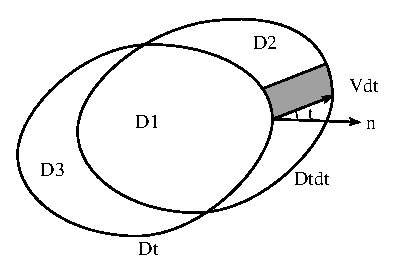
\includegraphics[scale=1]{../images/T1_Ch01-0002.eps}
\end{center}
\end{multicols}

Posant $J(t)=\iiint_{D(t)} \mathcal{A}(x,t) \ud v$, on peut écrire:
\begin{equation*}
    \begin{aligned}
        J(t+\ud t)-J(t) & =\iiint_{D(t+\ud t)} \mathcal{A}(x,t+\ud t) \ud v-\iiint_{D(t)} \mathcal{A}(x,t) \ud v\\
                        & =\iiint_{D_I} \left[\mathcal{A}(x,t+\ud t)-\mathcal{A}(x,t)\right] \ud v+\iiint_{D_{II}} \mathcal{A}(x,t+\ud t) \ud v-\iiint_{D_{III}} \mathcal{A}(x,t) \ud v\\
                        & =\left[\iiint_{D} \frac{\partial \mathcal{A}}{\partial t}(x,t) \ud v\right]\ud t+ \left[\iint_{\partial D} \mathcal{A}\vec{V}\cdot\vec{n} \ud s\right]\ud t
    \end{aligned}
\end{equation*}
en remarquant que pour $II$ ou $III$, l'élément de volume $\ud v$ (hachuré sur la figure ci-contre) est donné par:
\begin{equation*}
    \ud v=\pm V \ud t \cdot \ud S \cdot \cos\theta = \pm \vec{V}\cdot\vec{n} \ud S \ud t
\end{equation*}
On trouvera des démonstrations plus détaillées et plus rigoureuses dans \cite{Germain-62,Germain-73,Mandel-66,Gontier-69} entre autres.

En utilisant le théorème de la divergence (Annexe~\ref{Ann:A}) et la formule donnant la dérivée particulaire $\mathcal{A}$:
\begin{equation*}
    \frac{\ud \mathcal{A}}{\ud t}=\frac{\partial \mathcal{A}}{\partial t}+\mathcal{A}_{,i}V_i
\end{equation*}
(où on a utilisé la convention de sommation et la notation $f_{,i}=\partial f/\partial x_i$ -- voir Annexe~\ref{Ann:A}), on peut transformer~\eqref{eq:Ch01-005} en:
\begin{equation}
    \frac{\ud}{\ud t}\iiint_{D} \mathcal{A} \ud v=\iiint_{D}\left\{\frac{\partial\mathcal{A}}{\partial t}+(\mathcal{A}V_i)_{,i}\right\} \ud v=\iiint_{D} \left\{\frac{\ud\mathcal{A}}{\ud t}+\mathcal{A}\dive\vec{V}\right\} \ud v
    \label{eq:Ch01-006}
\end{equation}
Par une hypothèse analogue au Postulat de Cauchy, on suppose que la densité surfacique $\alpha$ dépend uniquement du point considéré et de la normale $\vec{n}$: $\alpha(M,\vec{n})$.
Moyennant des hypothèses de continuité que nous ne préciserons pas davantage, on montre alors:

\begin{lem}
    \begin{enumerate}[(a)]
        \item $\alpha(M,-\vec{n}) =-\alpha(M,\vec{n})$
        \item En un point donné $M$, il existe un flux $\vec{a}(M)$ tel que:
        \begin{equation}
            \alpha(M,\vec{n}) =a_i(M)n_i=\vec{a}\cdot\vec{n}
            \label{eq:Ch01-007}
        \end{equation}
    \end{enumerate}
    \label{lem:Ch01-2}
\end{lem}

\begin{wrapfigure}[3]{l}{.2\textwidth}
    \vskip-1.5em
    \centering
    \psfrag{dS}{\scriptsize $\ud S$}
    \psfrag{n}{\scriptsize $\vec n$}
    \psfrag{-n}{\scriptsize $-\vec n$}
    \psfrag{e}{\scriptsize $\varepsilon$}
    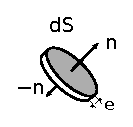
\includegraphics[clip]{../images/T1_Ch01-0003.eps}%\vspace{.2cm}
\end{wrapfigure}
\noindent Le point a) exprime simplement que ce qui rentre dans $D$ est l'opposé de ce qui en sort.
Lorsque $\varepsilon\rightarrow 0$, les seuls termes qui subsistent sont ceux relatifs aux deux faces, et \eqref{eq:Ch01-004} donne le point a).
\vspace{1em}

\begin{wrapfigure}[5]{r}{.2\textwidth}
    \vskip-2em
    \centering
    \psfrag{x1}{\scriptsize $x_1$}
    \psfrag{x2}{\scriptsize $x_2$}
    \psfrag{x3}{\scriptsize $x_3$}
    \psfrag{M0}{\scriptsize $M_0$}
    \psfrag{M1}{\scriptsize $M_1$}
    \psfrag{M2}{\scriptsize $M_2$}
    \psfrag{M3}{\scriptsize $M_3$}
    \psfrag{-e1}{\scriptsize $-\vec e_1$}
    \psfrag{-e2}{\scriptsize $-\vec e_2$}
    \psfrag{-e3}{\scriptsize $-\vec e_3$}
    \psfrag{n}{\scriptsize $\vec n$}
    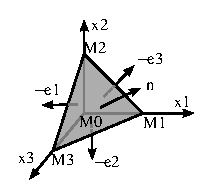
\includegraphics[clip]{../images/T1_Ch01-0004.eps}
\end{wrapfigure}
\noindent Pour démontrer le point b), on écrit~\eqref{eq:Ch01-004} pour un domaine $D$ en forme de tétraèdre $M_OM_1M_2M_3$, la face $M_1M_2M_3$ restant perpendiculaire au vecteur $\vec{n}$ donné.
Lorsque les dimensions du tétraèdre tendent vers zéro, la fonction $\alpha(M,\vec{n})$ reste à peu près constante en et ne dépend donc que de $\vec{n}$.

De plus, seule subsiste dans \eqref{eq:Ch01-004} l'intégrale de surface:
\begin{equation*}
    0=\iint_{M_1M_2M_3}\alpha(\vec{n}) \ud S+\iint_{M_0M_1M_2}\alpha(-\vec{e}_3) \ud S+ \iint_{M_0M_1M_3}\alpha(-\vec{e}_2) \ud S+\iint_{M_0M_2M_3}\alpha(-\vec{e}_1) \ud S
\end{equation*}
Si on note $S$ la surface de la face $M_1M_2M_3$ et $S_1$, $S_2$, $S_3$ celles de $M_OM_2M_3$, $M_OM_1M_3$, $M_0M_1M_2$ respectivement, il vient:
\begin{equation*}
    0 = \alpha(\vec{n})S+\alpha(-\vec{e}_3)S_3+\alpha(-\vec{e}_2)S_2+\alpha(-\vec{e}_1)S_1
\end{equation*}
soit, en utilisant a), en posant $a_i=\alpha(\vec{e}_i)$ et en remarquant que $S_i=\cos(\vec{e}_i,\vec{n})S=n_iS$:
\begin{equation*}
    \alpha(\vec{n})=a_in_i
\end{equation*}
Par utilisation de ces deux lemmes, on obtient la forme locale ou différentielle de la loi de conservation~\eqref{eq:Ch01-004}:
\begin{thm}
    \begin{equation}
        \frac{\ud \mathcal{A}}{\ud t} = -\mathcal{A}V_{i,i} + a_{i,i} + A
        \label{eq:Ch01-008}
    \end{equation}
    \label{thm:Ch01-1}
\end{thm}
\begin{proof}[Première démonstration]
    On utilise le théorème de la divergence pour transformer dans \eqref{eq:Ch01-004} l'intégrale de surface.
    Il vient:
    \begin{equation*}
        \iiint_D\left(\frac{\ud \mathcal{A}}{\ud t}+\mathcal{A}_{i,i}-a_{i,i}-A\right)\ud v=0
    \end{equation*}
    Cette égalité devant avoir lieu pour tout domaine $D$, on en tire la nullité de la quantité intégrée.
\end{proof}

\begin{proof}[Deuxième démonstration]
    On écrit la loi de conservation \eqref{eq:Ch01-004} en choisissant comme domaine $D$ un petit parallélépipède de côtés $h_1$, $h_2$, $h_3$.
    En utilisant le \tmp{lemme X}, on obtient en première approximation:
    \begin{align*}
        \frac{\ud}{\ud t}\iiint_D \mathcal{A} \ud v &= \iiint_D\left(\frac{\ud \mathcal{A}}{\ud t}+\mathcal{A}\dive \vec{V}\right)\ud v \\
        & \simeq \left(\frac{\ud \mathcal{A}}{\ud t}+\mathcal{A}\dive \vec{V}\right) h_1h_2h_3
    \end{align*}
    avec l'hypothèse $\iiint_D A \ud v =A h_1h_2h_3$.

    Pour l'intégrale de surface, on obtient:
    \begin{align*}
        \iint_{\partial D}\alpha \ud S & =\iint_{\partial D}\left(a_1n_1+a_2n_2+a_3n_3\right)\ud S \\
                                       & =\iint_{S_1}\quad \cdots \text{ permutation circulaire}\\
                                       & =\iint_{S_1} \left[a_1(x_1+h_1)-a_1(x_1)\right] \ud x_1 \ud x_2 + \cdots
    \end{align*}
    puisque $\vec{n}= (1,0,0)$ sur $S_1(x_1+h_1)$ et $\vec{n} = (-1,0,0)$ sur $S_1(x_1)$.
    Finalement il vient:
    \begin{equation*}
        \iint_{\partial D}\alpha \ud S=\left(\frac{\partial a_1}{\partial x_1}h_1\right)h_2h_3+\cdots=\frac{\partial a_i}{\partial x_i}h_1 h_2 h_3
    \end{equation*}
    d'où le résultat.
\end{proof}
\rput(11.8,8.5){%
\psfrag{x1}{\scriptsize $x_1$}
\psfrag{x2}{\scriptsize $x_2$}
\psfrag{x3}{\scriptsize $x_3$}
\psfrag{h1}{\scriptsize $h_1$}
\psfrag{h2}{\scriptsize $h_2$}
\psfrag{h3}{\scriptsize $h_3$}
\psfrag{e1}{\scriptsize $\vec e_1$}
\psfrag{e2}{\scriptsize $\vec e_2$}
\psfrag{e3}{\scriptsize $\vec e_3$}
\psfrag{-e1}{\scriptsize $-\vec e_1$}
\psfrag{-e2}{\scriptsize $-\vec e_2$}
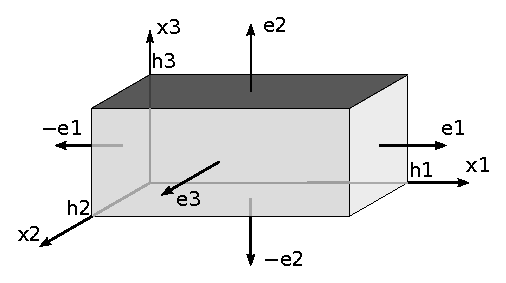
\includegraphics[width=7cm]{../images/T1_Ch01-0005.eps}}
Cette forme locale suppose la continuité des différentes quantités en cause.
En présence d'une surface de discontinuité $\Sigma$ se déplaçant à la vitesse $\vec{V}$, on définit la vitesse relative du choc $U$ par:
\begin{equation}
    U=(\vec{W}-\vec{V})\cdot \vec{N}
    \label{eq:Ch01-009}
\end{equation}
\begin{wrapfigure}[7]{l}{.3\textwidth}
    \psfrag{D}{\scriptsize $D$}
    \psfrag{S}{\scriptsize $\Sigma$}
    \psfrag{W}{\scriptsize $\vec W$}
    \psfrag{N}{\scriptsize $\vec N$}
    \includegraphics{../images/T1_Ch01-0006}
\end{wrapfigure}
On peut alors montrer (voir \cite{Germain-73}) que l'équation locale~\eqref{eq:Ch01-008} doit être complétée par une «~équation aux discontinuités~»:
\begin{equation}
    \llbracket\mathcal{A}U + a_iN_i\rrbracket = 0 
    \label{eq:Ch01-010}
\end{equation}
en désignant par $\llbracket h \rrbracket h(M^+)-h(M^-)$ le saut d'une grandeur à travers $\Sigma$.

L'application du Théorème~\ref{thm:Ch01-1} à la loi de conservation de la masse~\eqref{eq:Ch01-001} donne:
\begin{equation}
    \frac{\ud \rho}{\ud t}+\rho \dive \vec{V}=0
    \label{eq:Ch01-011}
\end{equation}
c'est l'équation de continuité.
Un calcul simple montre alors que:
\begin{equation*}
    \frac{\ud\mathcal{A}}{\ud t}+\mathcal{A}\dive \vec{V}=\rho\left\{\frac{1}{\rho}\frac{\ud \mathcal{A}}{\ud t}-\frac{1}{\rho^2}\mathcal{A}\frac{\ud \rho}{\ud t}\right\}=\rho \frac{\ud}{\ud t}\left(\frac{\mathcal{A}}{\rho}\right)
\end{equation*}
Le Lemme~\ref{lem:Ch01-1} et le Théorème~\ref{thm:Ch01-1} deviennent alors:
\begin{lem}[Lemme~\ref{lem:Ch01-1}']
    \begin{equation}
        \frac{\ud}{\ud t}\iiint_D\mathcal{A}\ud v=\iiint_D\rho\frac{\ud}{\ud t}\left(\frac{\mathcal{A}}{\rho}\right)(12)
        \label{eq:Ch01-012}
    \end{equation}
    \label{lem:Ch01-1p}
\end{lem}

\begin{thm}[Théorème~\ref{thm:Ch01-1}']
    \begin{equation}
        \rho\frac{\ud}{\ud t}\left(\frac{\mathcal{A}}{\rho}\right)=A+a_{i,i}(13)
        \label{eq:Ch01-013}
    \end{equation}
    \label{thm:Ch01-1p}
\end{thm}
Ces deux formes sont très utiles, car les quantités physiques sont plus souvent définies par leur densité massique $\mathcal{A}/\rho$ que volumique $\mathcal{A}$.
\subsection{Utilisation de la loi fondamentale} \label{ssec:Ch01-1.3}
L'application du Lemme~\ref{lem:Ch01-2} à la loi de conservation de la quantité de mouvement~\eqref{eq:Ch01-002} (en prenant $\alpha=T_i$ permet d'introduire le \emph{tenseur des contraintes} $\sigma_{ij}$
système de 9 quantités, tel que:
\begin{equation}
    T_i=\sigma_{ij}n_j
    \label{eq:Ch01-014}
\end{equation}
Le chapitre~\ref{chap:Ch02} sera consacré à l'étude de ce «~tenseur des contraintes~».

L'application du Théorème~\ref{thm:Ch01-1p} à la loi de conservation de la quantité de mouvement \eqref{eq:Ch01-002} donne alors \emph{l'équation du mouvement}:
\begin{equation}
    \rho\gamma_i=\rho\frac{\ud V_i}{\ud t}=\sigma_{ij,j}+f_i
    \label{eq:Ch01-015}
\end{equation}
où $\gamma_i$ désigne l'accélération:
\begin{equation}
    \gamma_i=\frac{\ud V_i}{\ud t}=\frac{\partial V_i}{\partial t}+V_{i,j}V_j
    \label{eq:Ch01-016}
\end{equation}
Dans la suite de ce cours, on s'intéressera essentiellement aux problèmes statiques.
L'équation du mouvement~\eqref{eq:Ch01-015} devient alors \emph{l'équation d'équilibre}:
\begin{equation}
    \sigma_{ij,j}+f_i=0
    \label{eq:Ch01-017}
\end{equation}
système de 3 équations scalaires ($i=1,2,3$):
\begin{equation}
    \begin{aligned}
        &\frac{\partial \sigma_{11}}{\partial x_1}+\frac{\partial \sigma_{12}}{\partial x_2}+\frac{\partial \sigma_{13}}{\partial x_3}+f_1=0\\
        &\frac{\partial \sigma_{21}}{\partial x_1}+\frac{\partial \sigma_{22}}{\partial x_2}+\frac{\partial \sigma_{23}}{\partial x_3}+f_2=0\\
        &\frac{\partial \sigma_{31}}{\partial x_1}+\frac{\partial \sigma_{32}}{\partial x_2}+\frac{\partial \sigma_{33}}{\partial x_3}+f_3=0
    \end{aligned}
    \label{eq:Ch01-018}
\end{equation}
qui traduisent localement l'équilibre du milieu continu.

La loi de conservation du moment cinétique s'étudie de la même manière: on applique le Théorème~\ref{thm:Ch01-1p} avec $\mathcal{A}/\rho=\varepsilon_{ijk}a_jV_k$, $\alpha=\varepsilon_{ijk}x_jT_k=\varepsilon_{ijk}x_j\sigma_{kl}n_l$ d'après \eqref{eq:Ch01-014}, et $A=\varepsilon_{ijk}x_jk_k$.
Il vient:
\begin{equation*}
    \rho \frac{\ud}{\ud t}(\varepsilon_{ijk}x_jV_k)=(\varepsilon_{ijk}x_j\sigma_{kl})_{,l}+\varepsilon_{ijk}x_jf_k
\end{equation*}
On développe cette relation en remarquant que:
\begin{equation*}
    \frac{\ud x_j}{\ud t}=V_j, \qquad x_{j,l}=\frac{\partial x_j}{\partial x_l}=\delta_{jl}
\end{equation*}
où $\delta_{jl}$ est le symbole de Kronecker:
\begin{equation*}
    \rho \varepsilon_{ijk}V_jV_k+\rho\varepsilon_{ijk}x_j\gamma_k=\varepsilon_{ijk}\delta_{jl}\sigma_{kl}+\varepsilon_{ijk}x_j\sigma_{kl,l}+ \varepsilon_{ijk}x_jf_k
\end{equation*}
Le premier terme disparaît car $\varepsilon_{ijk}$ est antisymétrique en $j$ et $k$.
Il reste:
\begin{equation*} 
    \varepsilon_{ijk}x_j(\rho\gamma_k-\sigma_{kl,l}-f_k)-\varepsilon_{ijk}\sigma_{jk}=0
\end{equation*}
Le premier terme s'annule d'après \eqref{eq:Ch01-015} et on obtient finalement $\varepsilon_{ijk}\sigma_{jk}=0$ c'est à dire:
\begin{equation}
    \sigma_{ij}=\sigma_{ji}
    \label{eq:Ch01-019}
\end{equation}
Le tenseur des contraintes est symétrique.
\begin{displaymath}
    \sigma_{12} = \sigma_{21}, \quad \sigma_{13}= \sigma_{31}, \quad \sigma_{23} = \sigma_{32}
\end{displaymath}
Ainsi la loi fondamentale de la dynamique est, sous forme locale, équivalente â l'équation du mouvement~\eqref{eq:Ch01-015} avec un tenseur des contraintes symétrique.
A nouveau ces résultats supposent la continuité des fonctions en cause.
En présence d'une surface de discontinuité $\Sigma$, il faut rajouter les relations de discontinuité \eqref{eq:Ch01-010} qui donnent:
\begin{itemize}
     \item pour la conservation de la masse:
        \begin{equation}
            \llbracket \rho U \rrbracket=0, \qquad \rho^+(\vec{W}-\vec{V}^+)\cdot \vec{N} =\rho^-(\vec{W}-\vec{V}^-)\cdot \vec{N}
            \label{eq:Ch01-020}
        \end{equation}
    \item pour la conservation de la quantité de mouvement:
    \begin{equation}
        \llbracket \rho U V_i +\sigma_{ij}N_j \rrbracket=0
        \label{eq:Ch01-021}
    \end{equation}
\end{itemize}
tandis que l'équation correspondante pour la conservation du moment cinétique est automatiquement vérifiée si \eqref{eq:Ch01-022} l'est.

Dans le cas statique, ces relations de discontinuité se ramènent à la seule condition:
\begin{equation}
    \llbracket\sigma_{ij}N_j\rrbracket=0,\qquad \vec{T}^+(\vec{N})=\vec{T}^-(\vec{N})
    \label{eq:Ch01-022}
\end{equation}
exprimant la continuité du vecteur $\vec{T}$.
Nous y reviendrons au chapitre~\ref{chap:Ch02}.
\section{Puissances virtuelles} \label{sec:Ch01-2}
\subsection{Théorème des puissances virtuelles} \label{ssec:Ch01-2.1}
Pour un système quelconque un mouvement virtuel est un mouvement possible de ce système mouvement «~virtuel~» par opposition au mouvement «~réel~» qui est celui qui se réalise effectivement par suite des efforts appliqués.
De même une «~vitesse virtuelle~» est une répartition de vitesse possible.
Pour un milieu continu déformable, une vitesse virtuelle sera définie par un champ de vitesses virtuelles $\displaystyle{\mathop{V}^{*}}_i(x)$, c'est à dire par un champ de vecteurs $\displaystyle{\mathop{V}^{*}}_i$ défini sur le solide $\Omega$.

Nous partons donc de l'équation du mouvement~\eqref{eq:Ch01-015} que nous multiplions par $\displaystyle{\mathop{V}^{*}}_i$ (il s'agit donc d'un produit scalaire), et nous intégrons sur le solide $\Omega$ tout entier:
\begin{equation*}
    \iiint_{\Omega}\rho\gamma_i {\mathop{V}^{*}}_i \ud v=\iiint_{\Omega}\sigma_{ij,j} {\mathop{V}^{*}}_i \ud v+\iiint_{\Omega}f_i {\mathop{V}^{*}}_i \ud v
\end{equation*}
mais en utilisant le
\begin{thmn}[Théorème de la divergence]
\begin{align*}
    \iiint_{\Omega}\sigma_{ij,j} {\mathop{V}^{*}}_i \ud v &= \iiint_{\Omega}[(\sigma_{ij} {\mathop{V}^{*}}_i)_{,j}-\sigma_{ij} {\mathop{V}^{*}}_{i,j}]\ud v\\
    &=\iint_{\partial \Omega}\sigma_{ij} {\mathop{V}^{*}}_i n_j \ud S-\iiint_{\Omega} \sigma_{ij} {\mathop{V}^{*}}_{i,j} \ud v
\end{align*}
\end{thmn}
Grâce à \eqref{eq:Ch01-014}, on retrouve dans le premier terme les efforts $\vec{T}$ appliqués sur $\Omega$ à travers $\partial \Omega$, tandis que, d'après la symétrie de $\sigma_{ij}$, on peut remplacer $\displaystyle{\mathop{V}^{*}}_{i,j}$ par sa partie symétrique $\displaystyle{\mathop{D}^{*}}_{ij}$ (Annexe~\ref{Ann:A}):
\begin{equation}
    {\mathop{V}^{{\ast}}}_{i,j}={\mathop{D}^{{\ast}}}_{ij}+{\mathop{\Omega}^{{\ast}}}_{ij},\qquad
    {\mathop{D}^{{\ast}}}_{ij}={\mathop{V}^{{\ast}}}_{i,j}+{\mathop{V}^{{\ast}}}_{j,i},\qquad
    {\mathop{\Omega}^{{\ast}}}_{ij}={\mathop{V}^{{\ast}}}_{i,j}-{\mathop{V}^{{\ast}}}_{j,i}
    \label{eq:Ch01-023}
\end{equation}
$\displaystyle{\mathop{D}^{{\ast}}}_{ij}$ est le tenseur taux de déformation et $\displaystyle{\mathop{\Omega}^{{\ast}}}_{ij}$ le tenseur au champ de vitesses virtuelles $\displaystyle{\mathop{V}^{{\ast}}}_i$.
Finalement on obtient:
\begin{equation}
    \everymath{\displaystyle}
    \begin{array}{cccc}
        \iiint_{\Omega}\rho\gamma_i {\mathop{V}^{\ast}}_i \ud v & = \iiint_{\Omega}f_i {\mathop{V}^{\ast}}_i \ud v & +                                                    \iint_{\partial\Omega}T_i {\mathop{V}^{\ast}}_i \ud S & -                           \iiint_{\Omega}\sigma_{ij} {\mathop{D}^{\ast}}_{ij} \ud v\\[7pt]
        \mathop{\mathcal{P}}^{\ast}{\!}^{(\text{a})} & = \mathop{\mathcal{P}}^{\ast}{\!}^{(\text{d})} & + \mathop{\mathcal{P}}^{\ast}{\!}^{(\text{c})} & + \mathop{\mathcal{P}}^{\ast}{\!}^{(\text{int})}\\[7pt]
        & =  & \mathop{\mathcal{P}}^{\ast}{\!}^{(\text{ext})} & + \mathop{\mathcal{P}}^{\ast}{\!}^{(\text{int})}
    \end{array}
    \label{eq:Ch01-024}
\end{equation}
en introduisant:
\begin{itemize}
    \item $\displaystyle \mathop{\mathcal{P}}^{\ast}{\!}^{(\text{a})}$: Puissance virtuelle des quantités d'accélération dans le champ de vitesses virtuelles $\displaystyle\mathop{V}^{\ast}$;
    \item $\displaystyle \mathop{\mathcal{P}}^{\ast}{\!}^{(\text{d})}$: Puissance virtuelle des efforts à distance;
    \item $\displaystyle \mathop{\mathcal{P}}^{\ast}{\!}^{(\text{c})}$: Puissance virtuelle des efforts à contact;
    \item $\displaystyle \mathop{\mathcal{P}}^{\ast}{\!}^{(\text{ext})} = \mathop{P}^{\ast}{\!}^{(\text{d})} + \mathop{P}^{\ast}{\!}^{(\text{c})}$: Puissance virtuelle des efforts extérieurs.
\end{itemize}
On retrouve donc l'énoncé classique des puissances virtuelles, à condition d'interpréter le terme complémentaire $\displaystyle \mathop{\mathcal{P}}^{\ast}{\!}^{(\text{int})}$ comme étant la puissance virtuelle des efforts intérieurs:
\begin{equation}
    \mathop{\mathcal{P}}^{\ast}{\!}^{(\text{int})}=-\iiint_\Omega \sigma_{ij}{\mathop{\mathcal{D}}^{\ast}}_{ij} \ud v
    \label{eq:Ch01-025}
\end{equation}
On peut s'assurer (voir \cite{Germain-62,Gontier-69}) que c'est une interprétation justifiée dans la mesure où elle généralise la puissance virtuelle des efforts intérieurs introduite en mécanique rationnelle pour un système de solides rigides.
En particulier, le lemme suivant montre que la puissance virtuelle des efforts intérieurs est nulle dans tout champ de vitesses rigidifiant, c'est à dire lorsque $\displaystyle {\mathop{V}^{\ast}}_i$ est le champ de vitesses d'un solide rigide. 

\begin{lem}
    Une condition nécessaire et suffisante pour qu'un champ de vitesses $\displaystyle {\mathop{V}^{\ast}}_i$ soit rigidifiant est que le tenseur taux de déformation associé $\displaystyle {\mathop{D}^{\ast}}_{ij}$ soit nul.
    \label{lem:Ch01-3}
\end{lem}
\begin{proof}
    \begin{description}
        \item[Condition nécessaire.] Un champ rigidifiant peut s'écrire 
            \begin{equation}
                \mathop{V}^{\ast}(M) = \vec{a} + \vec{b} \wedge \vec{OM},\quad {\mathop{V}^{\ast}}_i = a_i + \varepsilon_{ijk} b_j x_k
                \label{eq:Ch01-026}
            \end{equation}
            On obient alors directement
            \begin{displaymath}
                {\mathop{V}^{\ast}}_{i,j} = \varepsilon_{ijl}b_k = {\mathop{\Omega}^{\ast}}_{ij},\quad {\mathop{D}^{\ast}}_{ij} = 0
            \end{displaymath}
        \item[Condition suffisante.] Il faut montrer que la condition
            \begin{equation}
                {\mathop{D}^{\ast}}_{ij} = \frac{1}{2} \left( {\mathop{V}^{\ast}}_{i,j} + {\mathop{V}^{\ast}}_{j,i} \right) = 0
                \label{eq:Ch01-027}
            \end{equation}
            permet d'écrire~\eqref{eq:Ch01-026}.
            Nous démonstrerons ce résultat au chapitre~\ref{chap:Ch03} (paragraphe~\ref{ssec:Ch01-3.1}, Théorème~\ref{thm:Ch03-2}).
    \end{description}
\end{proof}
Nous avons donc démontré, à partir de la loi fondamentale, le
\begin{thmn}[Théorème des puissances virtuelles]
    Dans tout mouvement virtuel, la puissance virtuelle des quantités d'accélération est égale à la puissance virtuelle des efforts extérieurs et intérieurs
    \begin{equation}
        \mathop{\mathcal{P}}^{\ast}{\!}^{(\text{a})} = \mathop{\mathcal{P}}^{\ast}{\!}^{(\text{ext})} + \mathop{\mathcal{P}}^{\ast}{\!}^{(\text{int})}
        \label{eq:Ch01-028}
    \end{equation}
\end{thmn}

En particulier, si on prend comme champ de vitesses le champ des vitesse réelles, on obtien le
\begin{thmn}[Théorème de l'énergie cinétique]
    La dérivée par rapport au temps de l'énergie cinétique est égale à la puissance des efforts extérieurs et intérieurs
    \begin{align}
        \frac{\ud}{\ud t}\left( \frac{1}{2}\iiint_{\Omega} \rho V_iV_i \ud v\right) &= \iiint_{\Omega} f_i V_i \ud v &+ \iint_{\partial\Omega} T_i V_i \ud S &- \iiint_{\Omega} \sigma_{ij} D_ij \ud v \nonumber\\
        \frac{\ud K}{\ud t} &= \mathop{\mathcal{P}}^{\ast}{\!}^{(\text{ext})} &&+ \mathop{\mathcal{P}}^{\ast}{\!}^{(\text{int})}
        \label{eq:Ch01-029}
    \end{align}
\end{thmn}
\subsection{Le principe des puissances virtuelles} \label{ssec:Ch01-2.2}
Dans le cours de Mécanique Analytique, on a vu que l'on pouvait reconstruire la mécanique d'un système de solides à partir de l'énoncé des puissances virtuelles pris comme loi physique de départ.
La loi fondamentale est alors obtenue comme conséquence.
L'idée de départ est de caractériser un système d'efforts non plus par une densité volumique, surfacique ou autre, mais par la puissance que ce système d'efforts développe dans un mouvement virtuel quelconque.
En d'autres termes, un système d'efforts est une forme linéaire sur l'espace des vitesses virtuelles.
L'espace des efforts est donc dual de l'espace des vitesses virtuelles.

Nous postulons donc
\begin{Principe}[Principe des puissances virtuelles]
    La puissance virtuelle des quantités d'accélération est égale à la puissance virtuelle des efforts intérieurs et extérieurs
    \begin{equation}
        \mathop{\mathcal{P}}^{\ast}{\!}^{(a)} = \mathop{\mathcal{P}}^{\ast}{\!}^{(ext)} + \mathop{\mathcal{P}}^{\ast}{\!}^{(int)}
        \label{eq:Ch01-030}
    \end{equation}
    dans tout mouvement virtuel.
\end{Principe}


Toutes ces puissances virtuelles sont des formes linéaires sur l'espace $\mathop{\mathcal{V}}^{\ast}$ des champs de vitesses virtuelles:
\begin{itemize}
    \item La puissance des quantités d'accélération, $\mathop{\mathcal{P}}^{\ast}{\!}^{(a)}$, est imposée par le type de cinématique que l'on envisage.
    \item La puissance des efforts extérieurs, qui se décompose en deux parties:
        \begin{equation}
            \mathop{\mathcal{P}}^{\ast}{\!}^{(ext)} = \mathop{\mathcal{P}}^{\ast}{\!}^{(a)} + \mathop{\mathcal{P}}^{\ast}{\!}^{(c)}
            \label{eq:Ch01-031}
        \end{equation}
        (la puissance des efforts à distance $\mathop{\mathcal{P}}^{\ast}{\!}^{(d)}$ et la puissance des efforts de contact $\mathop{\mathcal{P}}^{\ast}{\!}^{(c)}$) est imposée par la nature des efforts extérieurs (donc connus) appliqués.
    \item La puissance des efforts intérieurs, par contre, pose davantage de problèmes:\\
        on sait que
\end{itemize}
\begin{Axiome}[Axiome]
    La puissance virtuelle des efforts intérieurs est nulle dans tout mouvement rigidifiant.
\end{Axiome}

Construire une théorie des milieux continus, c'est d'abord choisir l'espace $\mathop{\mathcal{V}}^{\ast}$ des champs de vitesses virtuelles, c'est ensuite choisir la forme des quatre formes linéaires $\mathop{\mathcal{P}}^{\ast}{\!}^{(a)}$, $\mathop{\mathcal{P}}^{\ast}{\!}^{(d)}$, $\mathop{\mathcal{P}}^{\ast}{\!}^{(c)}$ et $\mathop{\mathcal{P}}^{\ast}{\!}^{(int)}$.
Le reste de la théorie -- donc en particulier les équations du mouvement -- s'obtiennent par des calculs simples.

Considérons par exemple le cas de la mécanique des solides rigides: l'espace $\mathop{\mathcal{V}}^{\ast}$ des vitesses virtuelles est l'espace des champs de vitesses d'un solide, espace vectoriel de dimension 6.
Les formes linéaires $\mathop{\mathcal{P}}^{\ast}{\!}^{(a)}$ et $\mathop{\mathcal{P}}^{\ast}{\!}^{(ext)}$ (d'après l'axiome, $\mathop{\mathcal{P}}^{\ast}{\!}^{(int)}$ identiquement nulle) sont donc des éléments du dual de cet espace: l'espace des «~torseurs~».
Le principe des puissances virtuelles est donc équivalent à la loi fondamentale
\begin{equation}
    \left[ \mathcal{A} \right] = \left[ \mathcal{F}^{(ext)} \right]
    \label{eq:Ch01-032}
\end{equation}
où $\left[ \mathcal{A} \right]$ est le torseur des quantités d'accélération et $\left[ \mathcal{F}^{(ext)} \right]$ le torseur des efforts extérieurs.

De manière générale, la mécanique des milieux continus peut être construite indifféremment à partir des lois de conservation, comme nous l'avons fait au paragraphe~\ref{ssec:Ch01-1.1}, ou à partir du principe des puissances virtuelles, comme nous le ferons au paragraphe~\ref{ssec:Ch01-2.3}.
L'approche des puissances virtuelles présente cependant un double avantage:
\begin{enumerate}
    \item Elle est beaucoup plus systématique, et permet donc une généralisation plus facile lorsque l'on veut sortir du cadre des milieux continus classiques, pour étudier par exemple les milieux avec micro-structure évoqués au paragraphe~\ref{ssec:Ch01-1.1} cas des cristaux liquides ou bien les matériaux électromagnétiques.
    \item Elle met clairement en évidence la relation entre la description cinématique et la schématisation des efforts: plus on raffine la description cinématique, plus il faut raffiner la schématisation des efforts, et réciproquement.
        Par exemple, dans le cas du solide rigide, on voit clairement que la schématisation des efforts par des torseurs est liée à la cinématique du solide rigide: deux répartitions d'efforts différentes conduisant au même torseur sont équivalentes, car elles développent la même puissance dans tout mouvement possible.
\end{enumerate}

Pour ce cours élémentaire, nous ne partirons pas systématiquement de l'approche «~puissances virtuelles~», mais nous la mentionnerons régulièrement, et nous l'utiliserons pour mettre en évidence la dualité contraintes--déformations, ce qui sera une simple vérification en mécanique des milieux continus, mais jouera un rôle essentiel plus tard, en Résistance des Matériaux.

\subsection{Théorie du premier gradient} \label{ssec:Ch01-2.3}
Comme nous l'avons annoncé, nous allons ici reconstruire les équations fondamentales du paragraphe~\ref{ssec:Ch01-1.1} à partir du principe des puissances virtuelles.
En MMC classique, l'espace $\mathop{\mathcal{V}}^{\ast}$ est l'espace des champs de vecteurs sur le domaine $\Omega$ occupé par le solide.
Nous considérons une théorie du premier gradient, c'est à dire nous supposons que dans les formes linéaires définissant les puissances virtuelles, seul intervient le champ des vitesses virtuelles $\mathop{V}^{\ast}_i$ et son premier gradient $\mathop{V}^{\ast}_{i,j}$.

La schématisation des accélérations et des efforts extérieurs est la même que dans l'approche classique.
Nous prenons donc pour la puissance virtuelle des quantités d'accélération et des efforts extérieurs les formes suivantes
\begin{equation}
    \mathop{\mathcal{P}}^{\ast}{\!}^{(a)} = \iiint_{\Omega} \rho \gamma_i \mathop{V}^{\ast}_i \ud v \quad
    \mathop{\mathcal{P}}^{\ast}{\!}^{(d)} = \iiint_{\Omega} f_i \mathop{V}^{\ast}_i \ud v \quad
    \mathop{\mathcal{P}}^{\ast}{\!}^{(c)} = \iint_{\partial\Omega} T_i^e \mathop{V}^{\ast}_i \ud S
    \label{eq:Ch01-33}
\end{equation}
où $\gamma_i$ est l'accélération, $f_i$ les efforts à distance et $T_i^e$ les efforts de contact exercés sur le solide $\Omega$ à travers $\partial \Omega$ (alors que $T_i$ introduit au paragraphe~\ref{ssec:Ch01-1.1} était relatif à un sous-domaine quelconque $D\subset \Omega$: les lois de conservation sont imposées à tout domaine matériel $D$ alors que le principe des puissances virtuelles est écrit globalement pour le solide $\Omega$ tout entier).

La schématisation des efforts intérieurs, par contre, diffère de celle du paragraphe~\ref{ssec:Ch01-1.1} conformément à notre hypothèse d'une théorie du premier gradient, nous prenons
\begin{equation}
    \mathop{\mathcal{P}}^{\ast}{\!}^{(int)} = \iiint_{\Omega} \left( A_i \mathop{V}^{\ast}_i + B_{ij} \mathop{V}^{\ast}_{i,j} \right) \ud v
    \label{eq:Ch01-034}
\end{equation}
où les quantités $A_i$ et $B_{ij}$ caractérisent les efforts intérieurs.
En décomposant le tenseur gradient des vitesses $\mathop{V}^{\ast}_{i,j}$ en partie symétrique et antisymétrique, conformément à \eqref{eq:Ch01-023}, on peut remplacer \eqref{eq:Ch01-034} par
\begin{equation}
    \mathop{\mathcal{P}}^{\ast}{\!}^{(int)} = \iiint_{\Omega} \left( A_i \mathop{V}^{\ast}_i + \chi_{ij} \mathop{\Omega}^{\ast}_{ij} - \sigma_{ij} \mathop{D}^{\ast}_{ij} \right) \ud v
    \label{eq:Ch01-035} 
\end{equation}
avec $\sigma_{ij}$ symétrique et $\chi_{ij}$ antisymétrique.
D'autre part, on a vu (démonstration du Lemme~\ref{lem:Ch01-3}) que dans un mouvement rigidifiant on avait
\begin{equation}
    \mathop{V}^{\ast}_i = a_i \text{qcq}, \quad \tmp{\varepsilon_i k_j b_k \text{qcq}, \quad \mathop{I}^{\ast}_ij = 0}
    \label{eq:Ch01-036}
\end{equation}
L'axiome du paragraphe~\ref{ssec:Ch01-2.2} montre alors que $A_i$ et $\chi_{ij}$ doivent être nuls.
Il reste
\begin{equation}
    \mathop{\mathcal{P}}^{\ast}{\!}^{(int)} = -\iiint_{\Omega} \sigma_{ij} \mathop{D}^{\ast}_{ij} \ud v
    \label{eq:Ch01-037}
\end{equation}
Les efforts intérieurs sont donc caractérisés par un tenseur symétrique $\sigma_{ij}$.
Nous obtenons donc 
\begin{Principe}[Principe des puissances virtuelles en MMC]
    \begin{equation}
        \iiint_{\Omega} \rho \gamma_i \mathop{V}^{\ast}_i \ud v = \iiint_{\Omega} f_i \mathop{V}^{\ast}_i \ud v + \iint_{\partial \Omega} T_i^e \mathop{V}^{\ast}_i \ud S - \iiint_{\Omega} \sigma_{ij} \mathop{D}^{\ast}_{ij} \ud v
        \label{eq:Ch01-038}
    \end{equation}
    pour tout champ de vitesses virtuelles $\mathop{V}^{\ast}_i$.
\end{Principe}

Pour utiliser ce principe, il suffit maintenant de reprendre à l'envers le calcul du paragraphe~\ref{ssec:Ch01-3.1}:
\begin{align*}
    \iiint_{\Omega} \sigma_{ij} \mathop{D}^{\ast}_{ij} \ud v &= \iiint_{\Omega} \sigma_{ij} \mathop{V}^{\ast}_{i,j} \\
    &= \iint_{\partial \Omega} \sigma_{ij} \mathop{V}^{\ast}_{i} n_j \ud S - \iiint_{\Omega} \sigma_{ij,j} \mathop{V}^{\ast}_{i} \ud v
\end{align*}
ou l'on a utilisé la symétrie de $\sigma_{ij}$ et le théorème de la divergence.
On obtient alors
\begin{displaymath}
    \iiint_{\Omega} \left( \rho \gamma_i -f_i - \sigma_{ij,j} \right) \mathop{V}^{\ast}_i \ud v + \iint_{\partial \Omega} \left( \sigma_{ij} n_j - T_i^e \right) \mathop{V}^{\ast}_i \ud S = 0
\end{displaymath}
Ceci devant être vrai pour tout champ $\mathop{V}^{\ast}_i$, on en tire l'équation du mouvement \eqref{eq:Ch01-035} et la relation
\begin{equation}
    T_i^e = \sigma_{ij} n_j
    \label{eq:Ch01-039}
\end{equation}
qui est la relation~\eqref{eq:Ch01-014} pour $D=\Omega$. 

\section{Thermodynamique des milieux continus} \label{sec:Ch01-3}
\subsection{Conservation de l'énergie} \label{ssec:Ch01-3.1}
Le premier principe de la thermodynamique affirme que la variation de l'énergie totale (énergie interne + énergie cinétique) est, pour un domaine matériel $D$ quelconque, égale à la somme du travail des efforts extérieurs exercés sur $D$ et de la quantité de chaleur apportée à $D$
\begin{equation}
    \frac{\ud}{\ud t} \left( E + K \right) = \mathcal{P}^{(ext)} + Q
    \label{eq:Ch01-040}
\end{equation}
où 1'énergie cinétique $K$ et la puissance âes efforts extérieurs $\mathcal{P}^{(ext)}$ sont données par
\begin{equation}
    K = \iiint_{D} \frac{1}{2} \rho V_i V_i \ud v
    \label{eq:Ch01-041}
\end{equation}
\begin{equation}
    \mathcal{P}^{(ext)} = \iiint_{D} f_i V_i \ud v + \iint_{\partial D} T_i V_i \ud S
    \label{eq:Ch01-042}
\end{equation}
où l'énergie interne $E$ est définie par
\begin{equation}
    E = \iiint_{D} \rho e \ud v
    \label{eq:Ch01-043}
\end{equation}
en notant $e$ l'énergie interne par unité de masse, et où le taux de chaleur $Q$ apportée à $D$ résulte d'un apport volumique $r$ (rayonnnement) dans $D$ et d'un apport surfacique $h$ (conduction) à travers $\ud D$
\begin{equation}
    Q = \iiint_{D} r \ud v + \iint_{\partial D} h \ud S
    \label{eq:Ch01-044}
\end{equation}
Le premler principe de la thermodynamique conduit donc à la loi de consvation de l'énergie
\begin{equation}
    \frac{\ud}{\ud t} \iiint_D \rho \left( e + \frac{1}{2} V_i V_i \right) \ud v = \iiint_D \left( f_i V_i + r \right) \ud v + \iint_{\partial D} \left( T_i V_i + h \right) \ud S
    \label{eq:Ch01-045}
\end{equation}
qui rentre dans le cadre des lois de conservation définies au paragraphe~\ref{ssec:Ch01-1.1} en prenant
dans~\eqref{eq:Ch01-004}
\begin{table*}
    \centering
    \begin{tabular}[]{c|c|c}
        $\mathcal{A}$ & $\alpha$ & $A$ \\ \hline
        $\rho \left( e \frac{1}{2} V_i V_i \right)$ & $f_i V_i + r$ & $T_i V_i + h$
    \end{tabular}
\end{table*}

Compte-tenu de~\eqref{eq:Ch01-014}, le Lemme~\ref{lem:Ch01-2} du paragraphe~\ref{ssec:Ch01-1.2} permet d'introduire le vecteur flux de chaleur $\vec{q}$ qui permet de décrire les échanges de chaleur à travers $\partial D$ par
\begin{equation}
    h = - \vec{q} \cdot \vec{n} = -q_i n_i
    \label{eq:Ch01-046}
\end{equation}
L'application du Théorème~\ref{thm:Ch01-1p} donne alors
\begin{align*}
    & \rho \left( \frac{\ud e}{\ud t} + V_i \gamma_i \right) = \left( \sigma_{ij} V_i - q_j \right)_{,j} + f_i V_i + r\\
    & \rho \frac{\ud e}{\ud t} + \left( \rho \gamma_i - \sigma_{ij,j} - f_i \right) V_i = \sigma_{ij} V_{i,j} + r - q_{j,j}
\end{align*}
Le terme entre parenthèses disparaît d'après l'équation du mouvement \eqref{eq:Ch01-015}, et, compte-tenu de la symétrie de $\sigma_{ij}$, il reste
\begin{equation}
    \rho \frac{\ud e }{\ud t} = \sigma_{ij} D_{ij} + r - q_{j,j}
    \label{eq:Ch01-047}
\end{equation}
forme  locale du premier principe de la thermodynamique.

On aurait également pu obtenir \eqref{eq:Ch01-047} en utilisant le théorème de l'énergie cinétique du paragraphe~\ref{ssec:Ch01-2.1}.
Ce théorème permet en effet de remplacer \eqref{eq:Ch01-040} par
\begin{equation}
    \frac{\ud E}{\ud t} = Q - \mathcal{P}^{(int)}
    \label{eq:Ch01-048}
\end{equation}
ce  qui, d'après~\eqref{eq:Ch01-025}, donne, au lieu de \eqref{eq:Ch01-045},
\begin{equation}
    \frac{\ud}{\ud t} \iiint_{D} \rho e \ud v = \iiint_{D} \left( \sigma_{ij} D_{ij} + r \right) \ud v + \iint_{\partial D} h \ud S
    \label{eq:Ch01-049}
\end{equation}
et l'application du Lemme~\ref{lem:Ch01-2} et du Théorème~\ref{thm:Ch01-1p} à cette loi de conservation redonne directement \eqref{eq:Ch01-046} et \eqref{eq:Ch01-047}.

On pourrait également écrire l'équation aux discontinuités \eqref{eq:Ch01-010} associée à cette loi de conservation \eqref{eq:Ch01-045}
\begin{equation}
    \llbracket \rho \left( e + \frac{1}{2} V_i V_i \right) U + \left( \sigma_{ij} V_i + q_j \right) N_j \rrbracket = 0
    \label{eq:Ch01-050}
\end{equation}
mais elle sert peu en mécanique des solides.
Remarquons toutefois que l'on n'a pas le droit d'écrire cette relation aux discontinuités sur la loi de conservation~\eqref{eq:Ch01-049}, car on a utilisé pour obtenir~\eqref{eq:Ch01-045} le théorème de l'énergie cinétique, lequel suppose que le champ des vitesses est continu.

\subsection{Inégalité de Clausius-Duhem} \label{ssec:Ch01-3.2}
Le second principe de la thermodynamique qui, en thermostatique, pour un processus homotherme, s'écrit classiquement
\begin{equation}
    \ud S \geq \frac{1}{T} \ud Q
    \label{eq:Ch01-051}
\end{equation}
se généralise habituellement à la MMC sous la forme 
\begin{equation}
    \frac{\ud S}{\ud t} \geq \mathcal{S}^{(ext)} \quad \mathcal{S}^{(int)} = \frac{\ud S}{\ud t} - \mathcal{S}^{(ext)} \geq 0
    \label{eq:Ch01-052}
\end{equation}
exprimant que, pour tout domaine matériel $D$, le taux de ``production interne'' d'entropie $\mathcal{S}^{(int)}$ est positif, la production interne d'entropie étant définie comme étant la différence entre la variation de l'entropie du domaine $D$, définie par
\begin{equation}
    S = \iiint_{D} \rho \eta \ud v
    \label{eq:Ch01-053}
\end{equation}
où $\eta$ est l'entropie par unité de masse, et les ``échanges'' lT dT entropie avec l'extérieur, liés aux échanges de chaleur \eqref{eq:Ch01-044} par
\begin{equation}
    \mathcal{S}^{(ext)} = \iiint_{D} \frac{r}{\theta} \ud v + \iint_{\partial D} \frac{h}{\theta} \ud S
    \label{eq:Ch01-054}
\end{equation}
où $\theta$ est la température absolue.
Ainsi, compte-tenu de \eqref{eq:Ch01-046}, le second principe de la thermodynamique s'écrit sous la forme
\begin{equation}
    \frac{\ud}{\ud t} \iiint_D \rho \eta \ud v \geq \iiint_{D} \frac{r}{\theta} \ud v - \iint_{\partial D} \frac{q_i n_i}{\theta} \ud S
    \label{eq:Ch01-055}
\end{equation}
En utilisant le \tmp{Lemme~\ref{lem:Ch01-2p}} et le théorème de la divergence, on obtient la forme locale du second principe
\begin{align}
        \rho \frac{\ud \eta}{\ud t}  &\geq \frac{r}{\theta} - \left( \frac{q_i}{\theta} \right)_{,i} \nonumber\\
        \rho \theta \frac{\ud \eta}{\ud t}  &\geq r - q_{i,i} + \frac{1}{\theta} q_i\theta_{,i}
    \label{eq:Ch01-056}
\end{align}
En éliminant $r$ entre \eqref{eq:Ch01-047} et \eqref{eq:Ch01-056}, on obtient
\begin{equation}
    -\rho \left( \frac{\ud e}{\ud t} - \theta \frac{\ud \eta}{\ud t} \right) - \frac{1}{\theta}q_i \theta_{,i} + \sigma_{ij}D_{ij} \geq 0
    \label{eq:Ch01-057}
\end{equation}
c'est l'inégalité de Clausius-Duhem, que l'on peut aussi écrire sous la forme
\begin{equation}
    -\rho \left( \frac{\ud \psi}{\ud t} + \eta \frac{\ud \theta}{\ud t} \right) - \frac{1}{\theta}q_i \theta_{,i} + \sigma_{ij}D_{ij} \geq 0
    \label{eq:Ch01-058}
\end{equation}
où $\psi = e -\eta \theta$ est 1'énergie libre par unité de masse.

D'un point de vue purement mécanique, le second principe traduit l'irréversibilité et joue donc un rôle important.
En ``oubliant'' les variables thermiques, on peut réécrire \eqref{eq:Ch01-057} ou \eqref{eq:Ch01-058} sous la forme
\begin{equation}
    \left\{
    \begin{aligned}
        & \phi = -\rho \frac{\ud u}{\ud t} + \sigma_{ij} D_{ij} \geq 0\\
        & \sigma_{ij} D_{ij} = \rho \frac{\ud u}{\ud t} + \phi
    \end{aligned}
    \right.
    \label{eq:Ch01-059}
\end{equation}
où $u$ est l'énergie (interne ou libre, cela n'a plus d'importance, car on a oublié les variables thermiques) du matériau, et où $\phi$ est appelé dissipation.
En reportant dans le théorème de l'énergie cinétique, on obtient 
\begin{equation}
    \mathcal{P}^{(ext)} = \frac{\ud K}{\ud t} + \frac{\ud U}{\ud t} + \Phi^{(irr)} \qquad \Phi^{(irr)} = \iiint_{D} \phi \ud v \geq 0
    \label{eq:Ch01-060}
\end{equation}

La puissance des efforts extérieurs, c'est à dire la puissance dépensée, contribue à augmenter l'énergie cinétique et l'énergie du matériau, et est dissipée dans $\Phi^{(irr)}$.


\chapter{Le tenseur des contraintes} \label{chap:Ch02}
\section{Notions générales} \label{sec:Ch02-1}
\subsection{Vecteur contrainte tenseur des contraintes} \label{ssec:Ch02-1.1}
\begin{multicols}{2}
    \begin{center}
        \psfrag{D}{$D$}
        \psfrag{O}{$\Omega$}
        \psfrag{M1}{$M_1$}
        \psfrag{M2}{$M_2$}
        \psfrag{n}{$\vec{n}$}
        \psfrag{df}{$\vec{\ud f}$}
        \psfrag{T}{$\vec{T}$}
        \psfrag{Tt}{$\vec{T}_t$}
        \psfrag{Tn}{$\vec{T}_n$}
    \includegraphics{../images/T1_Ch02-0001}
    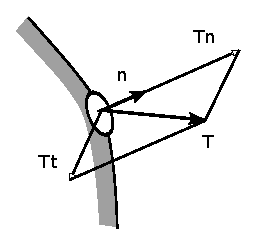
\includegraphics{../images/T1_Ch02-0002}
    \end{center}
\end{multicols}
Le vecteur contrainte caractérise les efforts de contact exercés à travers un élément de surface $\ud S$ de normale $\vec{n}$ sur une partie $D$ du milieu continu: le vecteur contrainte est défini par
\begin{equation}
    \vec{T}(\vec{n}) = \lim_{\ud S \rightarrow D} \frac{\ud \vec{f}}{\ud S} \qquad \ud \vec{f} = \vec{T}\left( \vec{n} \right) \ud D
    \label{eq:Ch02-001}
\end{equation}
Suivant le cas, il s'agit des efforts exercés sur $D$ par le reste du milieu continu (point $M_1$ -- il s'agit alors pour le solide $\Omega$ d'un effort intérieur) ou bien par l'extérieur (point $M_2$ -- effort extérieur pour $\Omega$).

Par convention on choisit pour $\vec{n}$ la normale extérieure au domaine $D$ sur lequel s'applique $\vec{T}$. 
Cette convention est à peu près universelle en MMC, à une exception près: la Mécanique des Sols, où l'on utilise la convention contraire.
Par convention également, on prend, en Mécanique des Solides, le zéro des contraintes pour la pression atmosphérique.
Les contraintes sont donc mesurées par rapport à cette pression atmosphérique.
Ainsi, si le solide est en contact avec un fluide à la pression $p$:
\begin{multicols}{3}
    \centering
    \psfrag{n}{$\vec{n}$}
    \psfrag{T}{$\vec{T}$}
    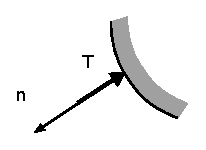
\includegraphics{../images/T1_Ch02-0003a}\\
    $p > p_{atm}$
    \columnbreak

    \psfrag{T}[c]{$\vec{T}=0$}
    
\includegraphics{../images/T1_Ch02-0003b}\\
    $p = p_{atm}$
    \columnbreak

    \psfrag{T}{$\vec{T}$}
    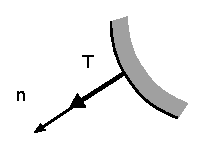
\includegraphics{../images/T1_Ch02-0003c}\\
    $p < p_{atm}$
\end{multicols}
\begin{equation}
    \vec{T} = -\left( p - p_{atm} \right) \vec{n}
    \label{eq:Ch02-002}
\end{equation}­ ­
La pression atmosphérique est d'ailleurs en général négligeable par rapport aux contraintes que l'on rencontre.

On projette le vecteur contrainte sur la normale et sur le plan perpendiculaire
\begin{equation}
    \vec{T} = T_{n}\vec{n} + \vec{T}_{t}
    \label{eq:Ch02-003}
\end{equation}
$T_n$ est la contrainte normale (algébrique), $\vec{T}_t$ est la contrainte tangentielle ou de cisaillement. 

Le vecteur contrainte est associé à un élément de surface de normale extérieure $\vec{n}$ -- on parle en général d'une «~facette~». 
Pour connaître «~l'état de contrainte~» en un point donné, il faut connaître les vecteurs contraintes associés à toutes les facettes, c'est à dire à tout vecteur unitaire $\vec{n}$.
Ici intervient le Lemme~\ref{lem:Ch01-2} du paragraphe~\ref{ssec:Ch01-1.2} qui permet de montrer que $\vec{T}$ dépend linéairement de $\vec{n}$.
Il existe donc une application linéaire -- le «~tenseur des contraintes~» -- faisant passer de $\vec{n}$ à $\vec{T}$
\begin{equation}
    \vec{T} = \mathbb{\sigma} \vec{n}
    \label{eq:Ch02-004}
\end{equation}
Le tenseur des contraintes est donc une application linéaire de l'espace vectoriel à trois dimensions $E_3$ dans lui-même.
Si l'on choisit une base orthonormée $\vec{e}_i$, cette application linéaire est représentée par une matrice d'éléments $\sigma_{ij}\ (i,\ j = 1,\ 2,\ 3)$  et la relation~\eqref{eq:Ch02-004} donne la relation matricielle
\begin{equation*}
    \begin{bmatrix}
        T_1\\
        T_2\\
        T_3
    \end{bmatrix}
    =
    \begin{bmatrix}
        \sigma_{11} & \sigma_{12} & \sigma_{13}\\
        \sigma_{21} & \sigma_{22} & \sigma_{23}\\
        \sigma_{31} & \sigma_{32} & \sigma_{33}
    \end{bmatrix}
    \begin{bmatrix}
        n_1\\
        n_2\\
        n_3
    \end{bmatrix}
\end{equation*}
c'est à dire \eqref{eq:Ch01-014}.
On obtient ensuite les équations d'équilibre \eqref{eq:Ch01-017} et la symétrie du tenseur des contraintes \eqref{eq:Ch01-019} à partir de la loi fondamentale. 
En d'autres termes, et c'est ce point de vue que l'on trouvera dans les traités classiques, on obtient~\eqref{eq:Ch02-004} en écrivant l'équilibre d'un tétraèdre, et en écrivant l'équilibre d'un parallélépipède on obtient 
\begin{itemize}
    \item à partir de l'équation de résultante, les équations d'équilibre~\eqref{eq:Ch01-017};
    \item à partir de l'équation de moment, la symétrie du tenseur des contraintes
\end{itemize}

De manière similaire, si $\Sigma$ est une surface de discontinuité -- par exemple une interface entre deux matériaux différents -- alors, l'équilibre d'un disque aplati parallèle à $\Sigma$ donne la condition~\eqref{eq:Ch01-022} de continuité du vecteur contrainte associé à $\Sigma$
\begin{equation}
    \sigma_{ij}^+ N_j = \sigma_{ij}^- N_j
    \label{eq:Ch02-005}
\end{equation}

Si l'on considère un second repère orthonormé $\vec{e}_i^{\prime}$ relié au premier par une matrice de passage $Q_{ij}$ orthogonale
\begin{equation}
    \vec{e}_i^{\prime} = Q_{ij} \vec{e}_j,\ Q_{ij}Q_{ik} = Q_{ji}Q_{ki} = \delta_{jk}
    \label{eq:Ch02-006}
\end{equation}
alors les composantes des vecteurs $\vec{T}$ et $\vec{n}$ et d'un tenseur $\sigma_{ij}$ se transforment (Annexe~\ref{Ann:A}) par
\begin{equation}
    T_i^{\prime} = Q_{ij} T_j,\ \sigma_{ij}^{\prime} = Q_{ik}Q_{jl} \sigma_{kl}
    \label{eq:Ch02-007}
\end{equation}

Les composantes $\sigma_{11}$, $\sigma_{22}$, $\sigma_{13}$, \dots sont les composantes des vecteurs contraintes associés aux facettes normales à $\vec{e}_1$, $\vec{e}_2$, $\vec{e}_3$.
\begin{multicols}{2}
    \begin{center}
        \psfrag{x1}{$x_1$}
        \psfrag{x2}{$x_2$}
        \psfrag{x3}{$x_3$}
        \psfrag{s11}{$\sigma_{11}$}
        \psfrag{s12}{$\sigma_{12}$}
        \psfrag{s13}{$\sigma_{13}$}
        \psfrag{s23}{$\sigma_{23}$}
        \psfrag{s22}{$\sigma_{22}$}
        \psfrag{s33}{$\sigma_{33}$}
        \includegraphics{../images/T1_Ch02-0004}
    \end{center}
    \columnbreak
    \begin{center}
        \psfrag{x1}{$x_1$}
        \psfrag{x2}{$x_2$}
        \psfrag{s11}{$\sigma_{11}$}
        \psfrag{s12}{$\sigma_{12}$}
        \psfrag{s22}{$\sigma_{22}$}
        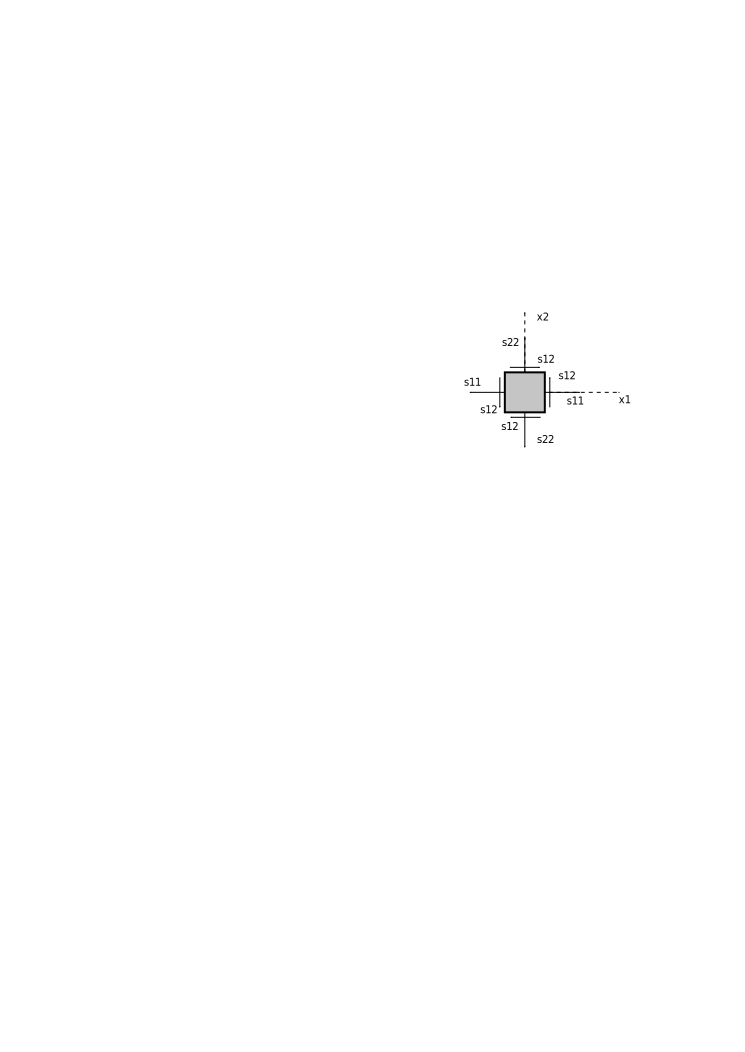
\includegraphics{../images/T1_Ch02-0005}
    \end{center}
\end{multicols}
Les composantes diagonales $\sigma_{11}$, $\sigma_{22}$, $\sigma_{33}$, sont donc des contraintes normales, tandis que les composantes non diagonales $\sigma_{12}$, $\sigma_{13}$, \dots sont des contraintes de cisaillement.
La symétrie du tenseur des contraintes $\sigma_{12} = \sigma_{21}$ exprime l'égalité de la contrainte de cisaillement associée à deux facettes perpendiculaires.
Peur cette raison, cette symétrie est souvent appelée «~principe de réciprocité des cisaillements~».

Dimensionnellement, une «~contrainte~» -- qu'il s'agisse d'une composante du vecteur contrainte ou du tenseur des contraintes -- est homogène à une force par unité de surface, donc à une pression.
L'unité SI, le Pascal ($1 Pa = 1 N/m^2$) étant très petite par rapport aux contraintes habituellement rencontrées, on utilise traditionnellement l'hectobar, le mégapascal et le $daN/mm$ (et chez les anglo-saxons, le p.s.i. \textit{pound per square inch}).
\begin{itemize}
    \item[] 1 daN/mm$^2$ = 1 hectobar = 10 MPa = $10^7$ Pa
\end{itemize}

\subsection{Contraintes principales invariants} \label{ssec:Ch02-1.2}
Le tenseur des contraintes est symétrique; on peut donc le diagonaliser.
Il existe trois directions principales orthogonales associées à trois valeurs propres $\sigma_1$, $\sigma_2$, $\sigma_3$,  appelées «~contraintes principales~».
\begin{equation}
    \sigma_{ij} e_j^{(1)} = \sigma_1 e_i^{(1)},\ \text{ etc.}
    \label{eq:Ch02-008}
\end{equation}
À partir de la décomposition~\eqref{eq:Ch02-003}, on voit qu'une condition nécessaire et suffisante pour qu'une direction soit principale pour $\mathbb{\sigma}$ est que la contrainte exercée sur la facette correspondante soit purement normale (pas de contrainte de cisaillement).
Dans le repère principal, la matrice représentative du tenseur des contraintes est diagonale.
Par abus de langage, on dit que le tenseur des contraintes est diagonal, et on écrit
\begin{equation}
    \mathbb{\sigma} = 
    \begin{bmatrix}
        \sigma_1 & 0 & 0 \\
        0 & \sigma_2 & 0 \\
        0 & 0 & \sigma_3
    \end{bmatrix}
    \label{eq:Ch02-009}
\end{equation}

Les contraintes principales s'obtiennent par résolution de l'équation caractéristique 
\begin{align}
    P_{\mathbb{\sigma}} & = \det
    \begin{bmatrix}
        \sigma_{11}-\lambda & \sigma_{12} & \sigma_{13}\\
        \sigma_{12} & \sigma_{22}-\lambda & \sigma_{23}\\
        \sigma_{13} & \sigma_{22} & \sigma_{33}-\lambda
    \end{bmatrix} \nonumber \\ 
        & = -\lambda^3 + I_1 \lambda^2 - I_2 \lambda + I_3
    \label{eq:Ch02-010}
\end{align}
où $I_1$, $I_2$, $I_3$	sont les invariants de $\mathbb{\sigma}$ définis par (Annexe~\ref{Ann:A})
\begin{equation}
    \left\{
    \begin{aligned}
        I_1 &= \sigma_{ii}= \sigma_1 + \sigma_2 + \sigma_3\\
        I_2 &= \frac{1}{2}\left( \sigma_{ii}\sigma_{jj} - \sigma_{ij}\sigma_{ij} \right) = \sigma_1\sigma_2 + \sigma_2\sigma_3 + \sigma_3\sigma_1\\
        I_3 &= \det \left( \sigma_{ij} \right) = \sigma_1\sigma_2\sigma_3
    \end{aligned}
    \right.
    \label{eq:Ch02-011}
\end{equation}
On 	décompose habituellement le tenseur des contraintes en déviateur et partie sphérique
\begin{equation}
    \sigma_{ij} = \sigma \delta_{ij} + s_{ij}
    \label{eq:Ch02-012}
\end{equation}
où  $\sigma$ est la partie sphérique
\begin{equation}
    \sigma = \frac{1}{3}I_1 = \frac{\sigma_{11} + \sigma_{22} + \sigma_{33}}{3} = \frac{\sigma_1 + \sigma_2 + \sigma_3}{3}
    \label{eq:Ch02-013}
\end{equation}
et où $s_{ij}$ est le déviateur (on appelle déviateur un tenseur de trace nulle)
\begin{equation}
    \left\{
    \begin{aligned}
        & s_{ii} = 0 \qquad s_{ij} = \sigma_{ij} + \frac{1}{3} \sigma_{kk} \delta_{ij}\\
        & s_{12} = \sigma_{12} \qquad s_{11}= \frac{2\sigma_{11} - \sigma_{22} -\sigma_{33}}{3}
    \end{aligned}
    \right.
    \label{eq:Ch02-014}
\end{equation}
Il est clair que le tenseur des contraintes et son déviateur ont mêmes directions principales, les contraintes principales déviatoires $s_1$, $s_2$, $s_3$ sont données par 
\begin{equation}
    s_1 = \frac{2\sigma_1 - \sigma_2 - \sigma_3}{3}
    \label{eq:Ch02-015}
\end{equation}
et les invariants $J_2$, $J_3$ (puisque $J_1 = 0$ par~\eqref{eq:Ch02-014}) du déviateur $s_{ii}$ sont donnés par 
\begin{equation}
    \left\{
    \begin{aligned}
        J_2 &= -\frac{1}{2}s_{ij}s_{ij}\\
        &= s_1 s_2 + s_2 s_3 + s_3 s_1\\
        &= -\frac{1}{2} \left( s_1^2 + s_2^2 + s_3^2 \right)\\
        &= -\frac{1}{6} \left[ \left( \sigma_1 - \sigma_2 \right)^2 + \left( \sigma_2 - \sigma_3 \right)^2 + \left( \sigma_3 -\sigma_1 \right)^2 \right]\\
        J_3 &= \det \left( s_{ij} \right)  = s_1 s_2 s_3
    \end{aligned}
    \right.
    \label{eq:Ch02-016}
\end{equation}
\subsection{États de contraintes particuliers} \label{ssec:Ch02-1.3}
Nous allons envisager divers cas particuliers correspondant à des états de contraintes remarquables. 
\subsubsection{État de tension ou compression hydrostatique}
\begin{equation}
    \mathbb{\sigma} = 
    \begin{bmatrix}
        \sigma & 0 & 0 \\
        0 & \sigma & 0 \\
        0 & 0 & \sigma
    \end{bmatrix}
    \begin{aligned}
        \text{tension si } & \sigma > 0\\
        \text{compression si } & \sigma < 0
    \end{aligned}
    \label{eq:Ch02-017}
\end{equation}
Les trois contraintes principales sont égales, le déviateur est nul, et toutes les directions sont principales.
Sur toute facette s'exerce donc une contrainte purement normale.
\begin{multicols}{2}
    \begin{center}
        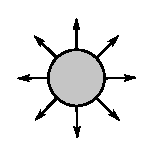
\includegraphics{../images/T1_Ch02-0006a}\\
        $\sigma > 0$ (tension)
    \end{center}
    \columnbreak
    \begin{center}
        \includegraphics{../images/T1_Ch02-0006b}\\
        $\sigma < 0$ (compression)
    \end{center}
\end{multicols}
C'est l'état de contraintes qui existe dans les fluides à l'équilibre, d'où la terminologie «~hydrostatique~».
\subsubsection{État  de  contraintes  de  révolution}
\begin{equation}
    \mathbb{\sigma} = 
    \begin{bmatrix}
        \sigma_1 & 0 & 0 \\
        0 & \sigma_2 & 0 \\
        0 & 0 & \sigma_3
    \end{bmatrix}
    \label{eq:Ch02-018}
\end{equation}
Deux des contraintes principales coïncident; les directions principales sont:
\begin{enumerate}
    \item la direction $x_1$, pour $\sigma_1$;
    \item toute direction du plan $\left( x_2, x_3 \right)$, pour $\sigma_2$.
\end{enumerate}
La décomposition en déviateur et partie sphérique devient 
\begin{equation}
    \mathbb{\sigma} = \sigma 
    \begin{bmatrix}
        1 & 0 & 0\\
        0 & 1 & 0\\
        0 & 0 & 1
    \end{bmatrix}
    +
    s
    \begin{bmatrix}
        1 & 0 & 0\\
        0 & -\frac{1}{2} & 0\\
        0 & 0 & -\frac{1}{2}
    \end{bmatrix},\ 
    \sigma = \frac{\sigma_1 + 2\sigma_2}{3} \quad s = \frac{2\left( \sigma_1 - \sigma_2 \right)}{3}
    \label{eq:Ch02-019}
\end{equation}
\begin{multicols}{2}
    \begin{center}
        \psfrag{s1}{$\sigma_1$}
        \psfrag{s2}{$\sigma_2$}
        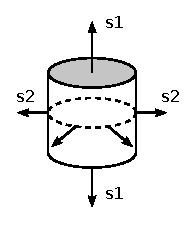
\includegraphics{../images/T1_Ch02-0007a}
    \end{center}
    \columnbreak
    \begin{center}
        \psfrag{s1}{$\sigma_1$}
        \psfrag{s2}{$\sigma_2$}
        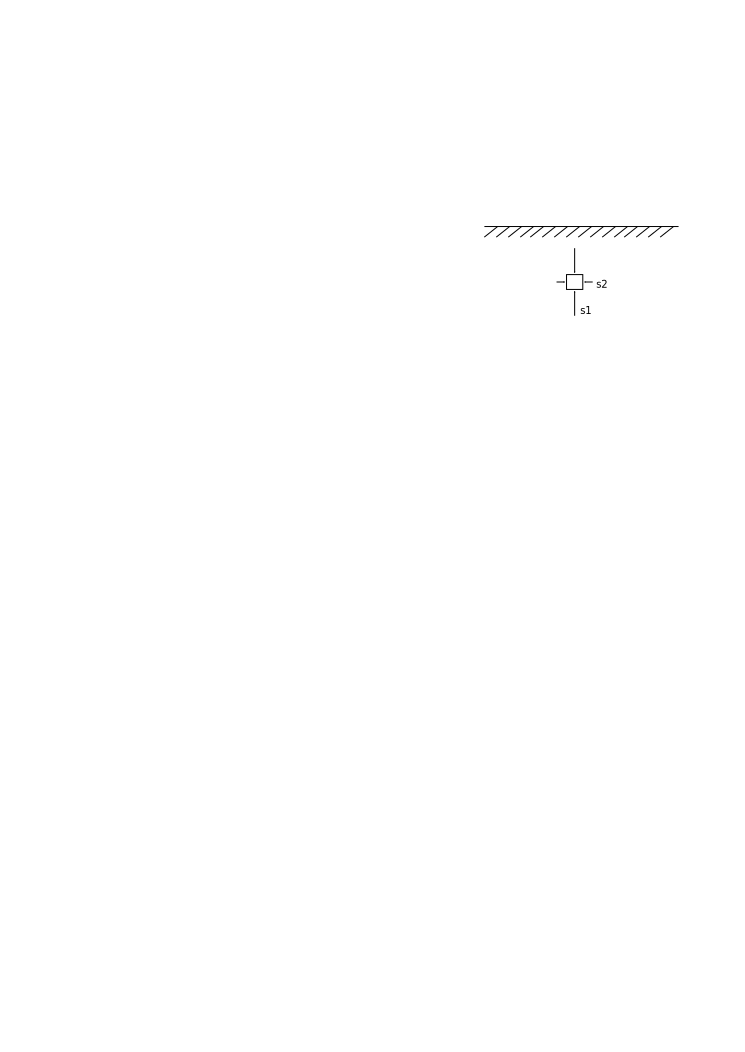
\includegraphics{../images/T1_Ch02-0007b}
    \end{center}
\end{multicols}
C'est l'état de contrainte qui se réalise avec $\sigma_1 <\sigma_2 < 0$ dans le sol en profondeur. 
\subsubsection{État de traction ou compression uniaxiale}
\begin{minipage}[l]{.2\textwidth}
\begin{center}
    \psfrag{s}{$\sigma$}
    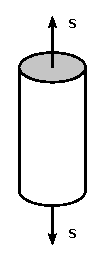
\includegraphics{../images/T1_Ch02-0008}
\end{center}
\end{minipage}
\begin{minipage}[r]{.8\textwidth}
\begin{equation}
    \mathbb{\sigma} = 
    \begin{bmatrix}
        \sigma & 0 & 0 \\
        0 & 0 & 0 \\
        0 & 0 & 0
    \end{bmatrix}
    \begin{aligned}
        \text{traction si } & \sigma > 0\\
        \text{compression si } & \sigma < 0
    \end{aligned}
    \label{eq:Ch02-020}
\end{equation}
C'est un cas particulier du précédent avec $\sigma_2 = 0$ (pas de contrainte latérale). 
C'est l'état de contrainte le plus facile à réaliser expérimentalement: il suffit d'exercer une force longitudinale sur un barreau (essai  de  traction).
\end{minipage}
\subsubsection{État de cisaillement pur}
\begin{equation}
    \mathbb{\sigma} = 
    \begin{bmatrix}
        0 & \tau & 0 \\
        \tau & 0 & 0 \\
        0 & 0 & 0
    \end{bmatrix}
    \label{eq:Ch02-021}
\end{equation}
État de contrainte purement déviatoire.
Les directions principales sont l'axe $x_3$ ($\sigma_3= 0$) et les bissectrices des axes $x_1$, $x_2$ (contraintes principales $+\tau$ et $-\tau$). 
\begin{multicols}{2}
    \begin{center}
        \psfrag{x1}{$x_1$}
        \psfrag{x2}{$x_2$}
        \psfrag{t}{$\tau$}
        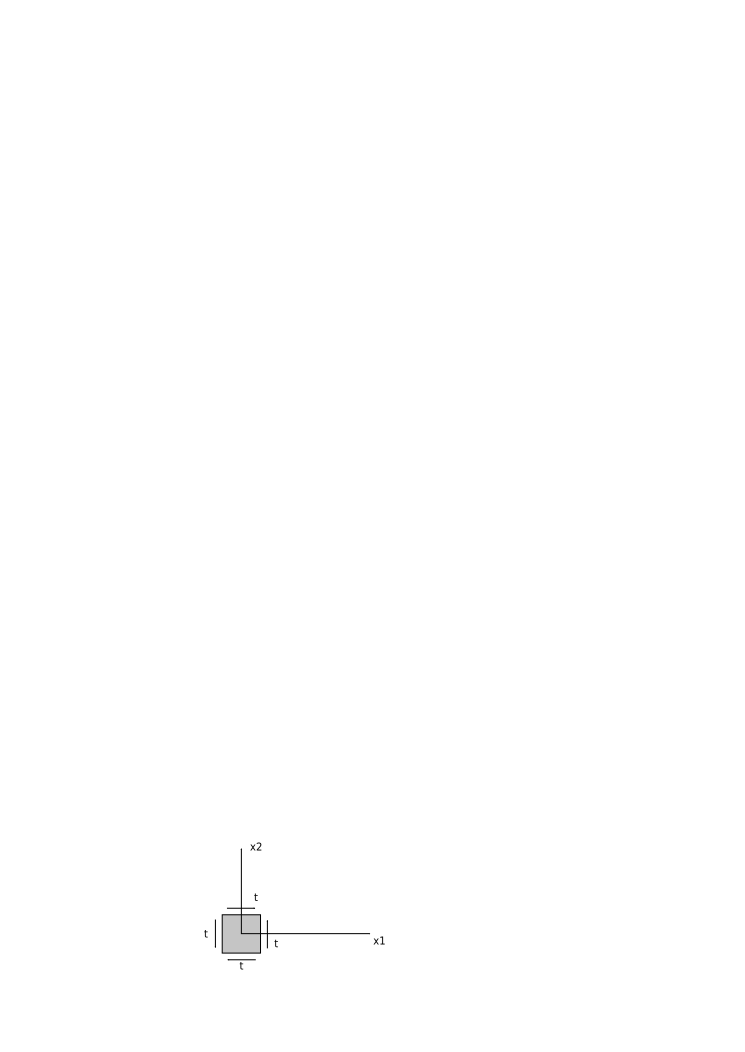
\includegraphics{../images/T1_Ch02-0009a}
    \end{center}
    \begin{center}
        \psfrag{x1}{$x_1$}
        \psfrag{x2}{$x_2$}
        \psfrag{t}{$\tau$}
        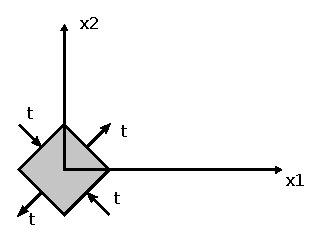
\includegraphics{../images/T1_Ch02-0009b}
    \end{center}
\end{multicols}
\subsubsection{État plan de contraintes}
\begin{equation}
    \mathbb{\sigma} = 
    \begin{bmatrix}
        \sigma_{11} & \sigma_{12} & 0 \\
        \sigma_{12} & \sigma_{22} & 0 \\
        0 & 0 & 0
    \end{bmatrix}
    \text{ ou }
    \begin{bmatrix}
        \sigma_{11} & \sigma_{12} & 0 \\
        \sigma_{12} & \sigma_{22} & 0 \\
        0 & 0 & \sigma_{33}
    \end{bmatrix}
    \label{eq:Ch02-022}
\end{equation}
\begin{minipage}[l]{.3\textwidth}
    \begin{center}
        \psfrag{x1}{$x_1$}
        \psfrag{x2}{$x_2$}
        \psfrag{s11}{$\sigma_{11}$}
        \psfrag{s22}{$\sigma_{22}$}
        \psfrag{s12}{$\sigma_{12}$}
        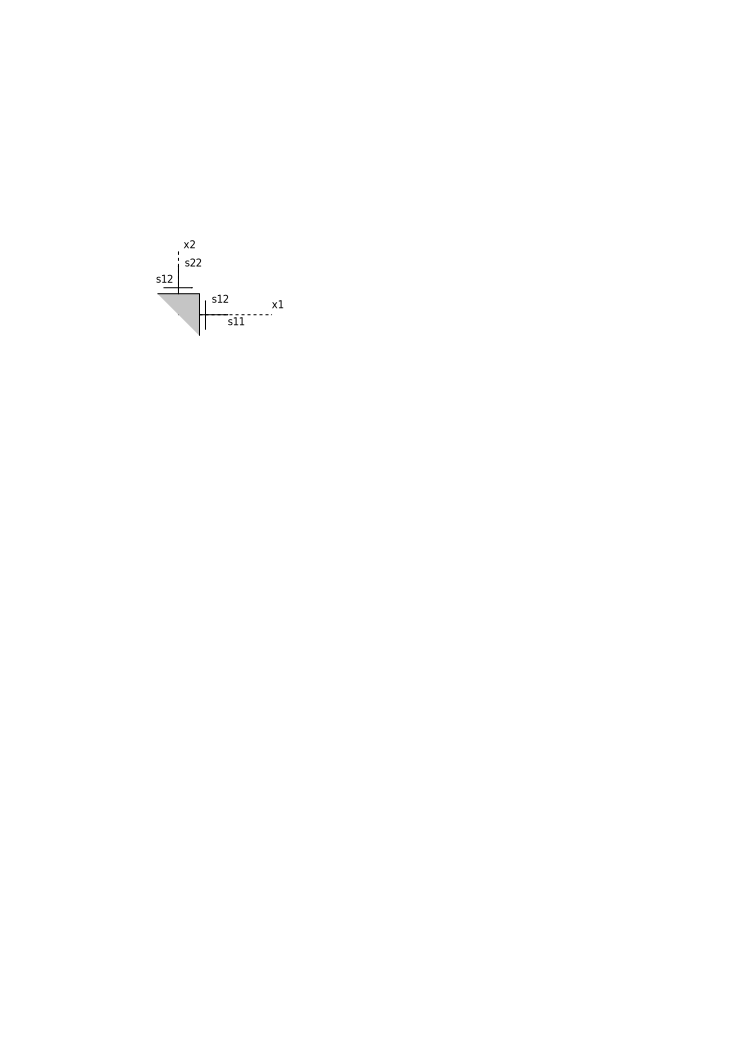
\includegraphics{../images/T1_Ch02-0010}
    \end{center}
\end{minipage}
\begin{minipage}[r]{.7\textwidth}
Les directions principales sont la direction $x_3$ et deux directions perpendiculaires du plan $x_1$, $x_2$.
Lorsque $\vec{n}$ varie dans le plan $x_1$, $x_2$, le vecteur contrainte reste dans le plan, et on peut se limiter au plan $x_1$, $x_2$.
Nous ferons l'étude complète au paragraphe~\ref{ssec:Ch02-3.2}.
\end{minipage}

\section{Représentations géométriques des contraintes} \label{sec:Ch2-2}
L'état de contraintes en un point donné est caractérisé par la valeur en ce point du tenseur des contraintes, c'est à dire par 6 nombres.
Pour visualiser cette entité, on a introduit diverses représentations géométriques.
\subsection{Quadriques des contraintes} \label{ssec:Ch02-2.1}
\subsubsection{Ellipsolde de Lamé}
C'est le lieu de l'extrémité du vecteur contrainte $\vec{T}$ lorsque $\vec{n}$ varie.
Si nous nous plaçons en repère principal, l'équation~\eqref{eq:Ch02-005} donne 
\begin{equation*}
    T_1 = \sigma_1 n_1 \qquad T_2 = \sigma_2 n_2 \qquad T_3 = \sigma_3 n_3
\end{equation*}
et, puisque le vecteur $vec{n}$ est unitaire 
\begin{equation}
    \frac{T_1^2}{\sigma_1^2} + \frac{T_2^2}{\sigma_2^2} + \frac{T_3^2}{\sigma_3^2} = 1
    \label{eq:Ch02-023}
\end{equation}
Le lieu de l'extrémité ($T_1$, $T_2$, $T_3$) est un ellipsoïde d'axes principaux sont les directions principales du tenseur des contraintes et de demi-axe les valeurs absolues des contraintes principales -- c'est l'el1ipsoïde de Lamé.
Mais cet ellipsoïde ne permet pas de visualiser le vecteur contrainte associé à une facette donnée.
\subsubsection{Quadrique directrice des contraintes normales}
Nous considérons la (ou les) quadrique(s) réelle(s) d'équation 
\begin{equation}
    \Phi(x) = \sigma_{ij} x_i x_j = \pm 1
    \label{eq:Ch02-024}
\end{equation}
C'est une (ou deux) quadrique(s) d'axes principaux les directions principales du tenseur des contraintes et de demi-axes ($1/\sqrt{|\sigma_1|}$, \ldots).
On les appelle quadriques directrices des contraintes, car elles permettent de construire le vecteur contrainte associé à une direction $\vec{n}$ quelconque par la construction suivante. 

\noindent\underline{Construction:} On mène de l'origine la demi-droite de direction $\vec{n}$, qui coupe la quadrique en un point $M$.  
\begin{itemize}
    \item la contrainte normale  est donnée  à  partir de  la longueur $OM=\rho$ par
        \begin{equation}
            \rho^2 |T_n| = 1
            \label{eq:Ch02-025}
        \end{equation}
    \item la direction du vecteur contrainte est donnée par la normale $\vec{N}$ à la quadrique en $M$. 
\end{itemize}
\begin{multicols}{2}
    \begin{center}
        \psfrag{x1}{$x_1$}
        \psfrag{x2}{$x_2$}
        \psfrag{x3}{$x_3$}
        \psfrag{n}{$\vec{n}$}
        \psfrag{N}{$\vec{N}$}
        \psfrag{M}{M}
        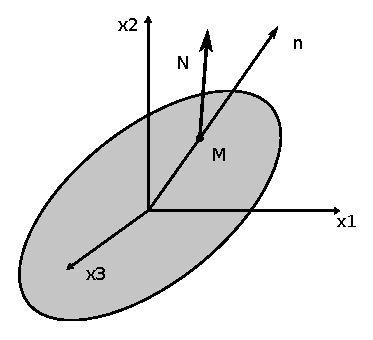
\includegraphics{../images/T1_Ch02-0011}
    \end{center}
    \columnbreak
    \begin{proof}
        On a $\vec{OM} = p \vec{n},\ x_i = p n_i$.
    En reportant dans~\eqref{eq:Ch02-024}, il vient
    \begin{displaymath}
        \rho^2 \sigma_{ij} n_i n_j = \pm 1
    \end{displaymath}
    qui donne~\eqref{eq:Ch02-025}, en remarquant que
    \begin{displaymath}
        T_n = \vec{T} \cdot \vec{n} = \sigma_{ij} n_i n_j
    \end{displaymath}
    La direction de la normale $\vec{N}$ à la quadrique donnée par le gradient de la fonction $\Phi$  est  
    \begin{displaymath}
        N_i = \lambda \frac{\partial \Phi}{\partial x_i} = 2\lambda \sigma_{ij} x_j = 2 \lambda \rho \sigma_{ij} n_j = 2 \lambda \rho T_i
    \end{displaymath}
    et $\vec{N}$ est proportionnel à $\vec{T}$.
    \end{proof}
\end{multicols}
Si toutes les contraintes principales sont de même signe, la forme quadratique 
\begin{equation}
    T_n = \sigma_{ij} n_i n_j
    \label{eq:Ch02-026}
\end{equation}
est définie positive ou négative, et \eqref{eq:Ch02-024} définit un ellipsoïde.
Si les contraintes principales sont certaines positives et d'autres négatives, alors $T_n$ peut être positif ou négatif, et \eqref{eq:Ch02-024} définit deux hyperboloïdes limités par le cône asymptote $T_n = 0$.
Enfin, si une contrainte principale est nulle, \eqref{eq:Ch02-024} définit un cylindre elliptique ou hyperbolique, suivant le signe des deux autres valeurs propres. 
\subsection{Espace des contraintes principales} \label{ssec:Ch02-2.2}
Le tenseur des contraintes (ou plus généralement tout tenseur symétrique) peut être caractérisé par les trois contraintes principales et l'orientation du repère principal.
Dans de nombreux cas, l'orientation du repère principal ne joue pas un rôle essentiel, et on pourra caractériser le tenseur des contraintes par les trois contraintes principales $\sigma_1$, $\sigma_2$, $\sigma_3$.
On peut donc représenter un tenseur des contraintes par un point d'un espace à trois dimensions $O\sigma_1\sigma_2\sigma_3$: au tenseur $\mathbb{\sigma}$ on associe le point $\Sigma$ ayant comme coordonnées les contraintes principales $\sigma_1$, $\sigma_2$, $\sigma_3$ de $\mathbb{\sigma}$ (le repère $O\sigma_1\sigma_2\sigma_3$ étant postulé orthonormé).

\begin{wrapfigure}[15]{l}{.55\textwidth}
    \begin{center}
        \psfrag{P}{$\Pi$}
        \psfrag{S}{$S$}
        \psfrag{O}{$O$}
        \psfrag{s1}{$\sigma_1$}
        \psfrag{s2}{$\sigma_2$}
        \psfrag{s3}{$\sigma_3$}
        \psfrag{E}{$\Sigma$}
        \psfrag{E'}{$\Sigma'$}
        \psfrag{D}{$\Delta$}
        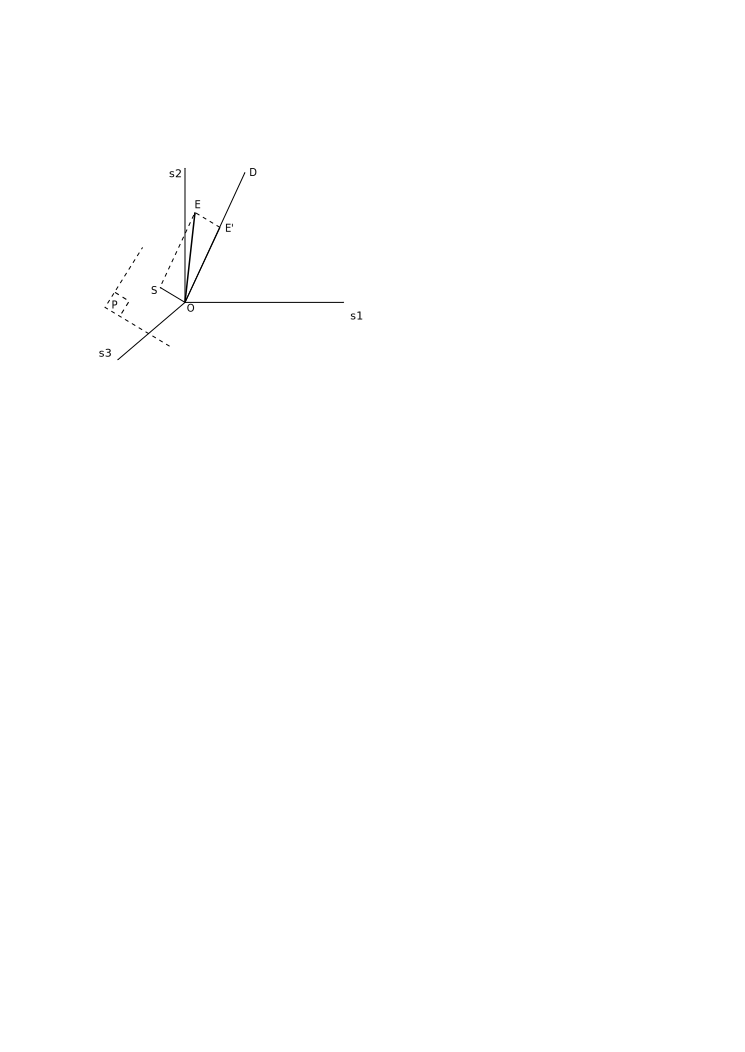
\includegraphics{../images/T1_Ch02-0012}
    \end{center}
\end{wrapfigure}
Cette représentation, très utile, exige néanmoins certaines précautions: on représente géométriquement l'espace des contraintes principales par un espace vectoriel mais ce n'est pas un espace vectoriel.
En particulier, les changements d'axes sont dépourvus de sens.
En particulier également, la somme de deux tenseurs $\sigma_{ij}^{(1)} + \sigma_{ij}^{(2)}$ ne correspond pas à la somme vectorielle (sauf dans le cas où les tenseurs $\sigma_{ij}^{(1)}$ et $\sigma_{ij}^{(2)}$ ont mêmes directions principales).
Enfin, un tenseur des contraintes est représenté, en toute rigueur, non pas par un point, mais par 6 points, car la numérotation des valeurs propres $\sigma_1$, $\sigma_2$, $\sigma_3$ est arbitraire. 

Dans cet espace, les tenseurs sphériques sont représentés par les points de l'«~axe hydrostatique $\Delta$~» (cosinus directeurs: $1/\sqrt{3},\ 1/\sqrt{3},\ 1/\sqrt{3}$).
Les déviateurs sont représentés par les points du plan déviatoire $\Pi$ , perpendiculaire en O à l'axe hydrostatique $\Delta$
\begin{equation}
    \sigma_1 + \sigma_2 + \sigma_3 = 0
    \label{eq:Ch02-027}
\end{equation}
La décomposition~\eqref{eq:Ch02-012} d'un tenseur en partie sphérique et déviateur correspond à la projection orthogonale sur $\Delta$ et $\Pi$.
En particulier, la projection sur $\Delta$ est caractérisée par la trace de $\mathbb{\sigma}$.
Dans le plan déviatoire $\Pi$ on trace 
\begin{center}
    \psfrag{Plan P}{Plan $\Pi$}
    \psfrag{S}{$S$}
    \psfrag{s1}{$\sigma_1$}
    \psfrag{s2}{$\sigma_2$}
    \psfrag{s3}{$\sigma_3$}
    \psfrag{r}{$r$}
    \psfrag{t}{$\theta$}
    \psfrag{h1}{$\vec{h}_1$}
    \psfrag{h2}{$\vec{h}_2$}
    \psfrag{h3}{$\vec{h}_3$}
    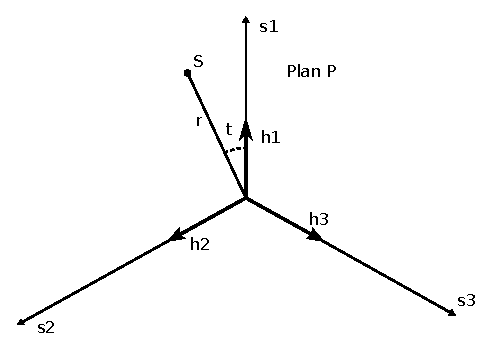
\includegraphics{../images/T1_Ch02-0013}
\end{center}
la projection des axes $O\sigma_1$, $O\sigma_2$, $O\sigma_3$, qui font entre eux un angle de $2\pi/3$ et un tenseur $\mathbb{\sigma}$ sera représenté par le point $S$
\begin{equation}
    \vec{OS} = \sigma_1 \vec{h}_1 + \sigma_2 \vec{h}_2 + \sigma_3 \vec{h}_3
    \label{eq:Ch02-028}
\end{equation}
$\vec{h}_1$, $\vec{h}_2$, $\vec{h}_3$ étant les trois vecteurs unitaires portés par les axes $O\sigma_1$, $O\sigma_2$, $O\sigma_3$ -- ou plutôt par leurs projections, mais nous les notons encore $O\sigma_1$, $O\sigma_2$, $O\sigma_2$, $O\sigma_3$.
En particulier, on vérifie bien que le point $S$ ainsi construit caractérise le déviateur, puisque, si l'on rajoute à $\mathbb{\sigma}$ un tenseur sphérique arbitraire, le point $S$ ne change pas, car $\vec{h}_1 + \vec{h}_2 + \vec{h}_3 = 0$.

On peut alors montrer que la position du point $S$ est complètement caractérisée par les deux invariants $J_2$ et $J_3$ introduits par~\eqref{eq:Ch02-016}.
Plus précisément, un calcul direct montre que les coordonnées polaires $\left( r,\ \theta \right)$ de $S$ sont données par 
\begin{equation}
    r = \sqrt{-3J_2},\ \cos 3 \theta = \frac{3\sqrt{3}}{2}\frac{J_3}{J_2^{3/2}}
    \label{eq:Ch02-029}
\end{equation}
Le second invariant $J_2$ détermine la distance $OS$, c'est à dire «~l'intensité~» du déviateur, tandis que le troisième invariant $J_3$ détermine son orientation. 
Plus précisément, on constate que l'on a 
\begin{align}
    3\theta &= \pm \arccos \left( \frac{3\sqrt{3}}{2} \frac{J_3}{J_2^{3/2}} \right) + 2 k \pi\nonumber\\
    \theta &= \pm \frac{1}{3}\arccos \left( \frac{3\sqrt{3}}{2} \frac{J_3}{J_2^{3/2}} \right) + \frac{2 k \pi}{3}
\end{align}
\begin{wrapfigure}[9]{r}{.4\textwidth}
    \begin{center}
        \psfrag{s1}{$\sigma_1$}
        \psfrag{s2}{$\sigma_2$}
        \psfrag{s3}{$\sigma_3$}
        \psfrag{S1}{$S_1$}
        \psfrag{S2}{$S_2$}
        \psfrag{S3}{$S_3$}
        \psfrag{S4}{$S_4$}
        \psfrag{S5}{$S_5$}
        \psfrag{S6}{$S_6$}
        \psfrag{O}{$O$}
        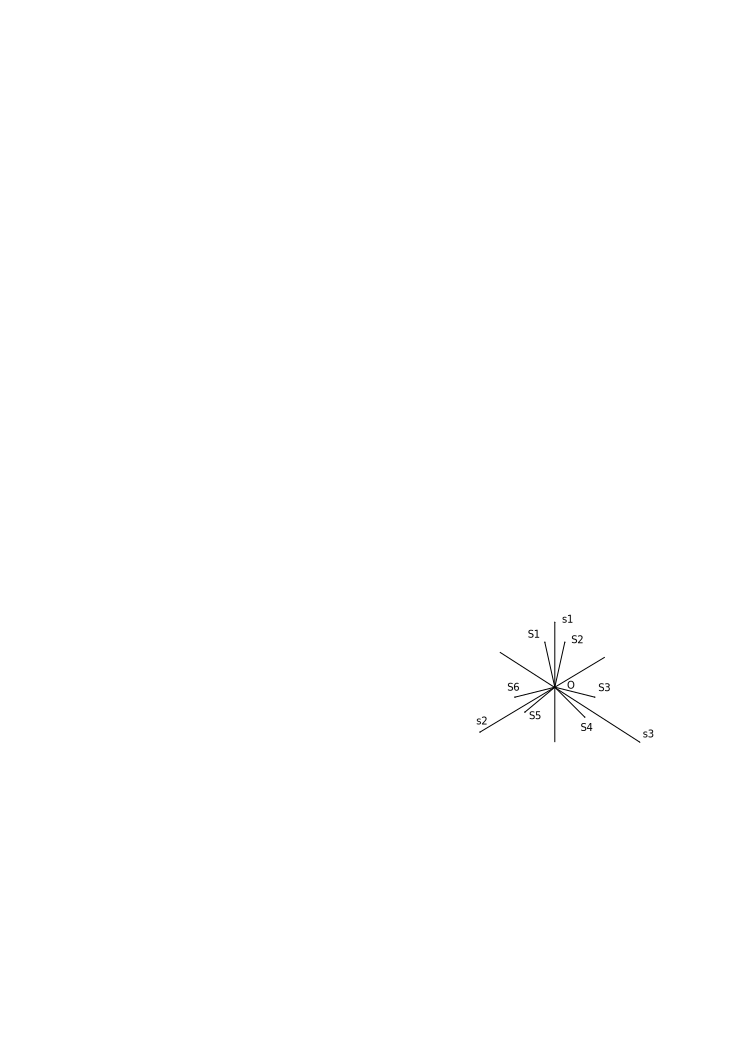
\includegraphics{../images/T1_Ch02-0014}
    \end{center}
\end{wrapfigure}
ce qui donne les 6 points $S$ correspondant aux 6 numérotations possibles des trois valeurs propres. 
Si l'on impose par exemple $\sigma_1 > \sigma_2 > \sigma_3$ alors on se restreint au quartier $O\sigma_1\sigma_3^{\prime}$ et le point $S$ est complètement défini. 

Finalement, on constate que la position du point $\Sigma$ dans l'espace des contraintes principales est complètement caractérisée par $I_1$, $J_2$, $J_3$: $I_1$ fixe la projection sur $\Delta$, $J_2$ la distance à $\Delta$ et $J_3$ l'orientation de la projection de $O\Sigma$ sur $\Pi$.

\section{Représentation de Mohr} \label{sec:Ch02-3}
\subsection{Tricercle de Mohr} \label{ssec:Ch02-3.1}
La représentation de Mohr est une représentation dans le plan des contraintes normales et tangentielles. 
On porte en abscisse la contrainte normale (algébrique) et en ordonnée le module de la contrainte tangentielle.
\begin{center}
    \psfrag{s1}{$\sigma_1$}
    \psfrag{s2}{$\sigma_2$}
    \psfrag{s3}{$\sigma_3$}
    \psfrag{M1}{$M_1$}
    \psfrag{M2}{$M_2$}
    \psfrag{M3}{$M_3$}
    \psfrag{M}{$M$}
    \psfrag{O}{$O$}
    \psfrag{Tt}{$|\vec{T}_t|$}
    \psfrag{Tn}{$T_n$}
    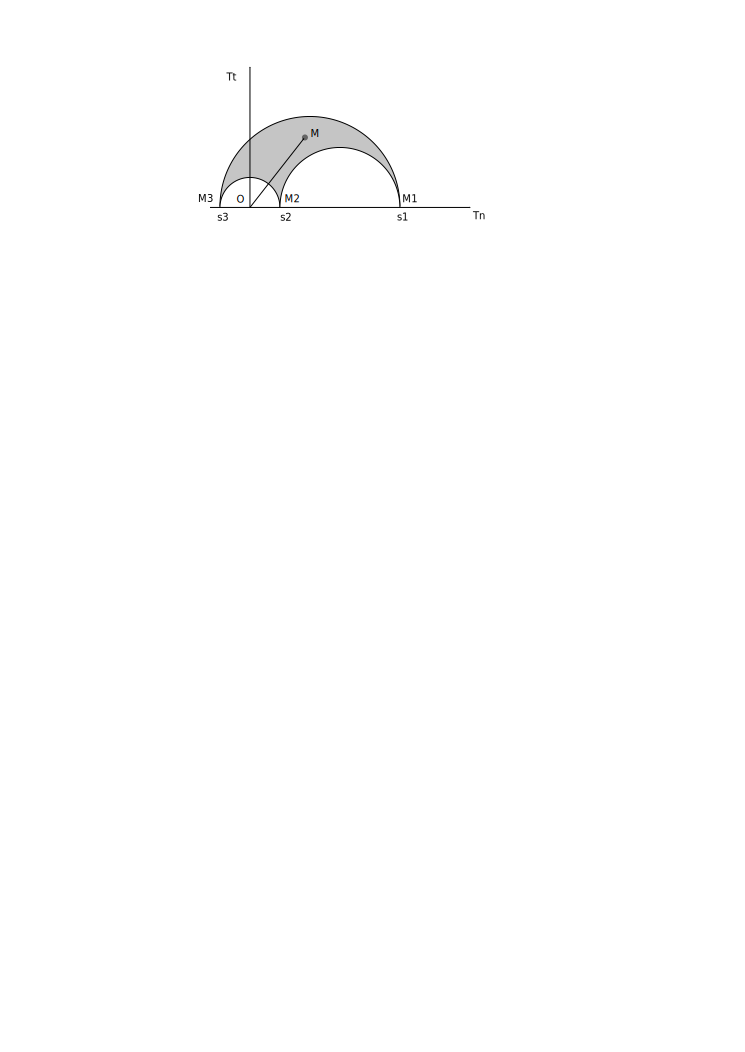
\includegraphics{../images/T1_Ch02-0015}
\end{center}
On obtient ainsi un point $M$ pour chaque facette, et on cherche le lieu de ces points lorsque l'on fait varier la facette.
Pour faire les calculs, on se place en repère principal du tenseur des contraintes et on suppose les valeurs propres rangées par ordre décroissant, $\sigma_3 < \sigma_2 < \sigma_1$.
Les points $M_1$, $M_2$ et $M_3$ correspondant aux facettes normales aux directions principales sont sur l'axe des contraintes normales.
Pour une facette quelconque, on a
\begin{displaymath}
    T_1 = \sigma_1 n_1 \quad T_2 = \sigma_2 n_2 \quad T_3 = \sigma_3 n_3
\end{displaymath}
qui permet de calculer $T_n = T_i n_i$ et $|T|^2 = T_n^2 + T_t^2$
\begin{equation}
    T_n = \sigma_1 n_1^2 + \sigma_2 n_2^2 + \sigma_3 n_3^2
    \label{eq:Ch02-031}
\end{equation}
\begin{equation}
    T_n^2 + T_t^2 = \sigma_1^2 n_1^2 + \sigma_2^2 n_2^2 + \sigma_3^2 n_3^2
    \label{eq:Ch02-032}
\end{equation}
Etant donnée une valeur de $T_n$ et de $T_t$, peut-on trouver une facette qui leur corresponde ?
Pour cela, il faut calculer $n_1$, $n_2$, $n_3$ à partir du système formé par \eqref{eq:Ch02-031}, \eqref{eq:Ch02-032} et la relation 
\begin{equation}
    1 = n_1^2 + n_2^2 + n_3^2
    \label{eq:Ch02-033}
\end{equation}
exprimant le fait que le vecteur $\vec{n}$ est unitaire.
On a donc un système linéaire en $n_1^2$, $n_2^2$, $n_3^2$, dont la solution est 
\begin{equation}
    n_1^2 = \frac{T_t^2 + \left( T_n - \sigma_2 \right)\left( T_n - \sigma_3 \right)}{\left( \sigma_1 - \sigma_2 \right)\left( \sigma_1 - \sigma_3 \right)}
    \label{eq:Ch02-034}
\end{equation}
et $n_2^2$, $n_3^2$, par permutation circulaire.
Géométriquement, on retrouve au dénominateur le produit scalaire $\vec{M_1M_2}\cdot\vec{M_1M_3}$ et au numérateur le produit scalaire $\vec{MM_2}\cdot \vec{MM_3}$.
On a donc 
\begin{equation}
    n_1^2 = \frac{\vec{MM_2} \cdot \vec{MM_3}}{\vec{M_1M_2} \cdot \vec{M_1M_3}},\quad n_2^2 = \frac{\vec{MM_1} \cdot \vec{MM_3}}{\vec{M_2M_1} \cdot \vec{M_2M_3}},\quad n_3^2 = \frac{\vec{MM_1} \cdot \vec{MM_2}}{\vec{M_3M_1} \cdot \vec{M_3M_2}}
    \label{eq:Ch02-035}
\end{equation}
Pour que cette solution soit satisfaisante, il faut vérifier que $n_1^2$, $n_2^2$ et $n_3^2$ sont positifs 
\begin{equation}
    n_1^2 \geq 0, n_2^2 \geq 0, n_3^2 \geq 0, 
    \label{eq:Ch02-036}
\end{equation}
Or, puisque $\sigma_3 < \sigma_2 < \sigma_1$, il est clair que
\begin{equation}
    \vec{M_1M_2} \cdot \vec{M_1M_3} \geq 0, \quad \vec{M_2M_1} \cdot \vec{M_2M_3} \leq 0, \quad \vec{M_3M_1} \cdot \vec{M_3M_2} \geq 0
    \label{eq:Ch02-037}
\end{equation}
Les conditions~\eqref{eq:Ch02-036} exigent donc 
\begin{equation}
    \vec{MM_2} \cdot \vec{MM_3} \geq 0, \quad \vec{MM_1} \cdot \vec{MM_3} \leq 0, \quad \vec{MM_1} \cdot \vec{MM_2} \geq 0
    \label{eq:Ch02-038}
\end{equation}
c'est à dire que les angles $\left( \vec{MM_2},\vec{MM_3} \right)$ et  $\left( \vec{MM_1},\vec{MM_2} \right)$ soient aigus et l'angle $\left( \vec{MM_1}, \vec{MM_3} \right)$ soit obtus, c'est à dire encore que le point $M$ soit à l'extérieur des deux demi-cercles de diamètres $M_1M_2$ et $M_2M_3$, et à l'intérieur du demi-cercle de diamètre $M_1M_3$.
Ainsi, quand $\vec{n}$ varie, le point $M$ reste dans la surface hachurée appelée -- tricercle de Mohr -- et qui devient un demi cercle si deux va­leurs propres coïncident, et un point pour un tenseur sphérique.

On constate d'autre part que $M$ décrit le demi cercle de diamètre $M_1M_3$ lorsque $\vec{n}$ varie dans le plan $\vec{e}_1, \vec{e}_3$ (car \eqref{eq:Ch02-035} montre que $n_2 = 0$  si et seulement si $\vec{MM_1}$ est orthogonal à $\vec{MM_3}$).
On voit également que le maximum de la contrainte de cisaillement (lorsque l'on fait varier la facette) est égale au rayon du plus grand cercle, c'est à dire à la demi différence des contraintes principales extrêmes
\begin{equation}
    |T_t|_{max} = \frac{\sigma_1 - \sigma_3}{2} = \frac{1}{2} \max_{i,j} |\sigma_i - \sigma_j|
    \label{eq:Ch02-039}
\end{equation}
On montrera au paragraphe~\ref{ssec:Ch02-3.2} que ce maximum est atteint lorsque $\vec{n}$ est bissectrice des directions principales.  

\subsection{Cercle de Mohr -- Pole} \label{ssec:Ch02-3.2}
Nous considérons maintenant un état plan de contraintes~\eqref{eq:Ch02-022}, et nous faisons varier $\vec{n}$, dans le plan $\left( x_1,x_2 \right)$.
On peut alors orienter la direction tangentielle à la facette en introduisant un vecteur unitaire $\vec{t}$ à $+\pi/2$ de $\vec{n}$.
La contrainte tangentielle $T_t$ devient donc une quantité algébrique, et la représentation dans le plan de Mohr permet de déterminer l'orientation du vecteur contrainte. 
\begin{multicols}{2}
    \begin{center}
        \psfrag{x1}{$x_1$}
        \psfrag{x2}{$x_2$}
        \psfrag{x1'}{$x_1'$}
        \psfrag{x2'}{$x_2'$}
        \psfrag{t}{$\theta$}
        \psfrag{Tt}{$T_t$}
        \psfrag{Tn}{$T_n$}
        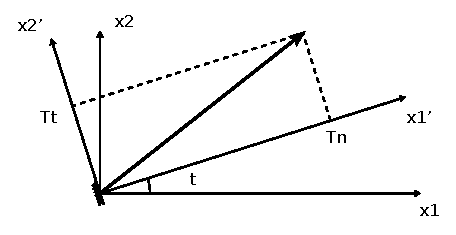
\includegraphics{../images/T1_Ch02-0016a}
    \end{center}
    \columnbreak
    \begin{center}
        \psfrag{Tn}{$T_n$}
        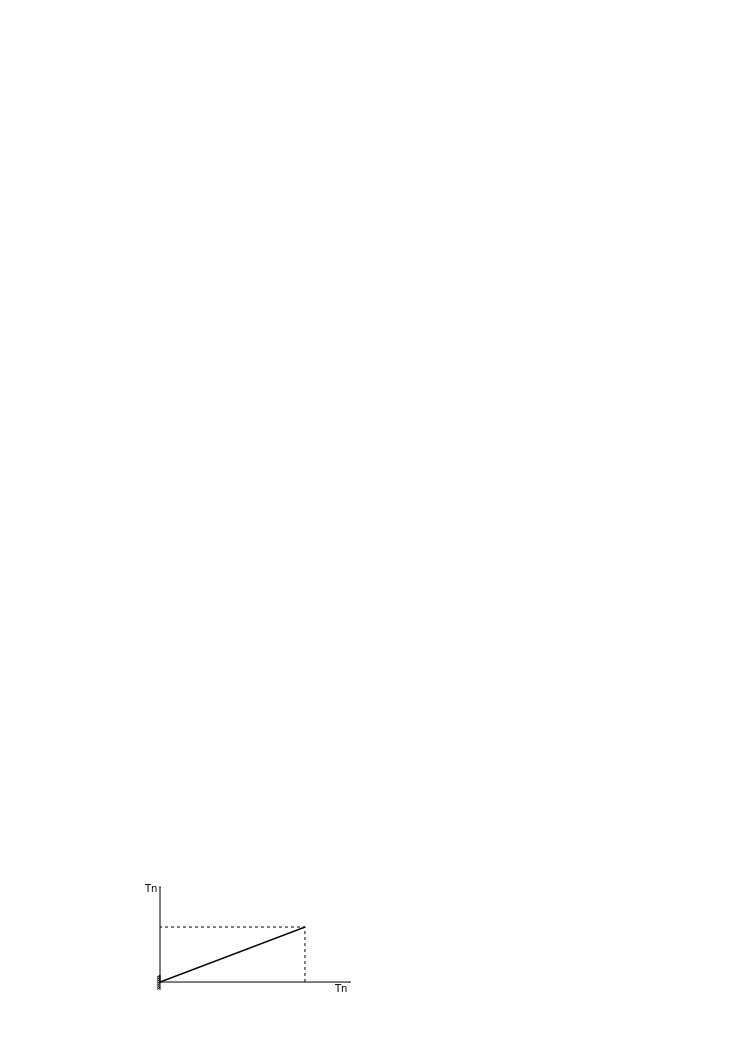
\includegraphics{../images/T1_Ch02-0016b}
    \end{center}
\end{multicols}
Pour calculer $T_n$ et $T_t$ on écrit
\begin{displaymath}
    \vec{n} = 
    \begin{bmatrix}
        \cos \theta\\
        \sin \theta
    \end{bmatrix}
    \quad
    \vec{t} = 
    \begin{bmatrix}
        -\sin \theta
        \cos \theta
    \end{bmatrix}
\end{displaymath}
on calcule le vecteur contrainte
\begin{equation}
    \left\{
    \begin{array}{lll}
        T_1 & = \sigma_{11} \cos \theta & + \sigma_{12} \sin \theta\\
        T_2 & = \sigma_{12} \cos \theta & + \sigma_{22} \sin \theta
    \end{array}
    \right.
    \label{eq:Ch02-040}
\end{equation}
et ensuite et en projetant $T_n$ et $T_t$ sur $\vec{n}$ et $\vec{t}$
\begin{equation}
    \left\{
    \begin{aligned}
        T_n &= \sigma_{11} \cos^2 \theta + 2 \sigma_{12} \cos \theta \sin \theta + \sigma_{22} \sin^2 \theta\\
            &= \frac{\sigma_{11} + \sigma_{22}}{2} + \frac{\sigma_{11} - \sigma_{22}}{2} \cos 2 \theta + \sigma_{12} \sin 2 \theta\\
        T_t &= \left(\sigma_{22}-\sigma_{11}\right) \cos \theta \sin \theta + \sigma_{12} \left( \cos^2\theta -\sin^2 \theta \right)\\
            &= -\frac{\left(\sigma_{11}-\sigma_{22}\right)}{2} + \sigma_{12} \cos 2 \theta
    \end{aligned}
    \right.
    \label{eq:Ch02-041}
\end{equation}
Les directions principales s'obtiennent en annulant la contrainte tangentielle $T_t = 0$:
\begin{equation}
    \tan 2 \theta_0 = \frac{2\sigma_{12}}{\sigma_{11} - \sigma_{22}}
    \label{eq:Ch02-042}
\end{equation}
ce qui définit $\theta_0$ à $k\pi/2$ près.
Nous choisissons $\theta_0$ en posant 
\begin{equation}
    \left\{
    \begin{aligned}
        \sigma_{12} &= \sqrt{\left( \frac{\sigma_{11} - \sigma_{12}}{2} \right)^2 + \sigma_{12}^2} \sin 2 \theta_0 \\
        \frac{\sigma_{11} - \sigma_{22}}{2} &= \sqrt{\left( \frac{\sigma_{11} - \sigma_{12}}{2} \right)^2 + \sigma_{12^2}} \cos 2 \theta_0
    \end{aligned}
    \right.
    \label{eq:Ch02-043}
\end{equation}
En reportant dans \eqref{eq:Ch02-043}, on obtient alors 
\begin{equation}
    \begin{aligned}
        T_n &= \frac{\sigma_{11} + \sigma_{22}}{2} + \sqrt{\left( \frac{\sigma_{11} - \sigma_{22}}{2} \right)^2 + \sigma_{12}^2} \cos 2 \left( \theta_0 - \theta \right)\\
        T_t &= \sqrt{\left( \frac{\sigma_{11} - \sigma_{22}}{2} \right)^2 + \sigma_{12}^2} \sin 2 \left( \theta_0 - \theta \right)
    \end{aligned}
    \label{eq:Ch02-044}
\end{equation}
Lorsque $\theta$ varie, le point $M$, représentant le vecteur contrainte dans le plan $T_n$, $T_t$, décrit un cercle de centre $\Omega$ et rayon $R$
\begin{equation}
    \Omega = \left( \frac{\sigma_{11}+\sigma_{22}}{2}, 0 \right), \ R = \sqrt{\left( \frac{\sigma_{11} - \sigma_{22}}{2} \right)^2 + \sigma_{12}^2}
    \label{eq:Ch02-045}
\end{equation}
\begin{center}
    \psfrag{Tt}{$T_t$}
    \psfrag{Tn}{$T_n$}
    \psfrag{A1}{$A_1$}
    \psfrag{A2}{$A_2$}
    \psfrag{B1}{$B_1$}
    \psfrag{B2}{$B_2$}
    \psfrag{M1}{$M_1$}
    \psfrag{M2}{$M_2$}
    \psfrag{2t}{$2\theta$}
    \psfrag{2t0}{$2\theta_0$}
    \psfrag{s11}{$\sigma_{11}$}
    \psfrag{s12}{$\sigma_{12}$}
    \psfrag{-s12}{$-\sigma_{12}$}
    \psfrag{s22}{$\sigma_{22}$}
    \psfrag{x1}{$x_1$}
    \psfrag{x2}{$x_2$}
    \psfrag{O}{$O$}
    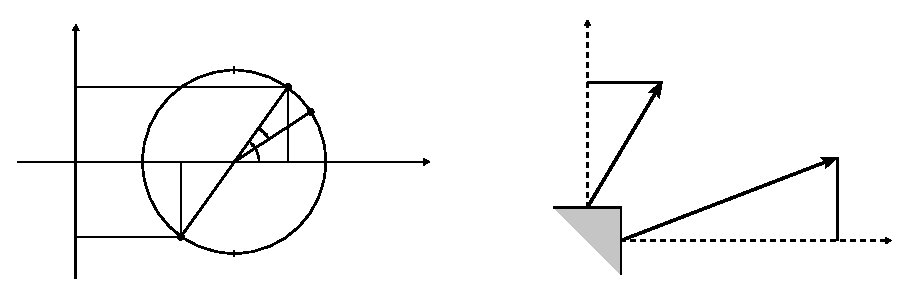
\includegraphics{../images/T1_Ch02-0017}
\end{center}
Les points  et $M_1\ \left( \sigma_{11},\ \sigma_{12} \right)$ et $M_2\ \left( \sigma_{22},\ -\sigma_{12} \right)$ correspondent à $\vec{n} = \vec{e}_1$ et $\vec{n}=\vec{e}_2$ respectivement. 
Pour obtenir le point $M$ correspondant à une normale $\vec{n}$ formant un angle $\theta$ avec $\vec{e}_1$, il faut tourner par rapport à $\Omega M_1$ d' un angle $2\theta$ dans le sens rétrograde.
Les points $A_1$ et $A_2$ correspondent aux directions principales, $\theta = \theta_0 + k\pi/2$ et les contraintes principales sont données par 
\begin{equation}
    \sigma_{1\text{ ou }2} = \frac{\sigma_{11} + \sigma_{22}}{2} \pm \sqrt{\left( \frac{\sigma_{11} - \sigma_{22}}{2} \right)^2 +\sigma_{12}^2}
    \label{eq:Ch02-046}
\end{equation}
Les points $B_1$ et $B_2$ correspondent aux directions de cisaillement maximal et sont donnés par $\theta = \theta_0 + \pi/4 + k\pi/2$, ce sont donc les bissectrices des directions principales, comme annoncé à la fin du paragraphe~\ref{ssec:Ch02-3.1}. 

Le point $M_1$ est appelé pôle du cercle de Mohr, et il permet une construction graphique du vecteur contrainte associé à une facette quelconque.
\begin{center}
    \psfrag{Tt}{$T_t$}
    \psfrag{Tn}{$T_n$}
    \psfrag{A1}{$A_1$}
    \psfrag{A2}{$A_2$}
    \psfrag{B1}{$B_1$}
    \psfrag{B2}{$B_2$}
    \psfrag{M}{$M$}
    \psfrag{M'}{$M'$}
    \psfrag{M1}{$M_1$}
    \psfrag{M1'}{$M_1'$}
    \psfrag{M2}{$M_2$}
    \psfrag{t}{$\theta$}
    \psfrag{2t}{$2\theta$}
    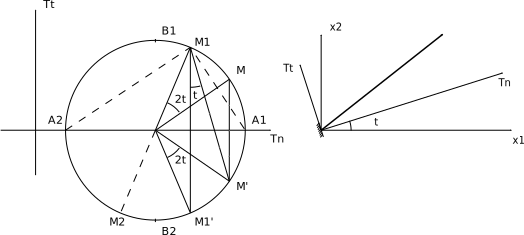
\includegraphics{../images/T1_Ch02-0018}
\end{center}
Pour obtenir le point $M$, c'est à dire le vecteur contrainte s'exerçant sur une facette inclinée de $\theta$ par rapport à la verticale, on utilise la construction suivante.
\begin{enumerate}
    \item On trace $M_1 M^{\prime}$ parallèle à la facette considérée, qui coupe le cercle de Mohr en $M^{\prime}$.
    \item $M$ est le symétrique de $M^{\prime}$ par rapport à l'axe des $T_n$.
\end{enumerate}
On en tire en particulier les directions principales $M_1 A_1$ et $M_1 A_2$ ainsi que les directions de contrainte tangentielle maximum $M_1 B_1$ et $M_1 B_2$. 


\chapter{Étude des déformations} \label{chap:Ch03}
\section{Grandes déformations} \label{sec:Ch03-1}
\subsection{Description de la déformation} \label{ssec:Ch03-1.1}
% Generated with LaTeXDraw 2.0.5
% Sun Nov 08 14:17:03 EST 2009
\scalebox{1} % Change this value to rescale the drawing.
{
\begin{pspicture}(0,-4)(14.744687,3.2425)
\psdots[fillstyle=solid,dotstyle=o](12.864688,1.5225)
\rput(4.8,0.7275){$\vec{\ud a}$}
\psdots[fillstyle=solid,dotstyle=o](5.0446873,0.3225)
\psdots[fillstyle=solid,dotstyle=o](5.4446874,1.3225)
\psline{->}(2.4646876,-1.2775)(2.4646876,2.3225)
\psline{->}(2.4646876,-1.2575)(6.8646874,-1.2575)
\psline{->}(2.4646876,-1.2575)(1.1046875,-2.8575)
\psbezier[linewidth=0.04](4.4646873,1.9225)(3.5646906,1.4866039)(3.1716466,0.11810785)(3.5246875,-0.8175)(3.8777285,-1.7531079)(4.424077,-2.4369879)(5.3646874,-2.0975)(6.305298,-1.7580122)(7.0475364,0.19629975)(6.6246877,1.1025)(6.2018385,2.0087004)(5.3646846,2.3583963)(4.4646873,1.9225)
\psline{->}(5.0646877,0.3225)(5.4446874,1.3425)
\psbezier[linewidth=0.02](5.0846877,0.3425)(6.0046873,1.2352536)(9.8046875,1.8425)(11.644688,0.9425)
\psdots[fillstyle=solid,dotstyle=o](11.644688,0.9225)
\psline{->}(11.684688,0.9425)(12.884687,1.5225)
\rput(6.909219,-1.5325){$x_1$}
\rput(3.1492188,2.4075){$x_2$}
\rput(1.8292187,-3.0325){$x_3$}
\rput(0.978125,0.1875){Repère fixe}
\rput(4.8392186,-0.0325){$M$}
\rput(4.8992186,1.5475){$M'$}
\rput(11.459219,0.5475){$M_t$}
\rput(13.119219,1.8475){$M_t'$}
\psbezier[linewidth=0.04](9.704687,-1.4775)(8.544687,0.0425)(11.924687,3.2225)(13.324688,2.4025)(14.724688,1.5825)(13.884687,1.1825)(12.964687,0.8225)(12.044687,0.4625)(10.864688,-2.9975)(9.704687,-1.4775)
\rput(4.845625,-2.6325){Configuration de référence}
\rput(10.955625,-2.6325){Configuration actuelle}
\rput(12.357187,-1.5125){instant $t$}
\psbezier[linewidth=0.02](5.4846873,1.3225)(7.2846875,2.4825)(10.884687,2.6425)(12.844687,1.5225)
\end{pspicture} 
}

Pour repérer la position d'une particule d'un milieu continu, il faut introduire un repère d'espace supposé fixe au cours du temps: un référentiel.
En général on choisit un référentiel galiléen, sinon il faut rajouter les forces d'inertie dans les forces de volume $f_i$.
Le mouvement est décrit par la fonction
\begin{equation}
    x_i = x_i \left( a_1, a_2, a_3, t \right) \quad i = 1, 2, 3
    \label{eq:Ch03-001}
\end{equation}
donnant la position à l'instant $t$, $M_t$, de la particule $M$ qui, dans la configuration de référence, occupe la position $\left( a_1, a_2, a_3 \right)$.
Les $x_i$ sont les variables eulériennes ou spatiales, les $a_i$ sont les variables lagrangiennes ou matérielles. 

Un vecteur matériel $\vec{\ud a} = \vec{MM'}$ devient après déformation $\vec{\ud x} = \vec{M_t M_t'}$
\begin{equation}
    \vec{\ud x_i} = \frac{\partial x_i}{\partial a_j} \ud a_j, \quad \vec{\ud x} = \mathbb{F} \vec{\ud a}
    \label{eq:Ch03-002}
\end{equation}
L'application linéaire tangente $\mathbb{F}$ qui à un vecteur matériel $\vec{\ud a}$ associe son déformation $\vec{\ud x}$ est appelée ``tenseur gradient de la déformation''.
Elle  caractérise la déformation ``locale'',  c'est-à-dire la déformation au  voisinage du point M.
Ce n'est pas cependant un mesure satisfaisante de la ``déformation'' au sens naïf du terme, car si le milieu a un mouvement de solide rigide, alors
\begin{equation}
    x_i = c_i (t) + Q_{ij} (t) a_j
    \label{eq:Ch03-003}
\end{equation}
où la matrice $Q_{ij}$ décrit une rotation et est donc orthogonale.
Le tenseur gradient de la déformation est alors donné par
\begin{equation}
    F_{ij} (a,t) = Q_{ij} (t)
    \label{eq:Ch03-004}
\end{equation}
alors qu'il n'y a manifestement pas de déformation au sens naïf du terme (variation de longueur ou variation d'angle).
En fait, le tenseur gradient de la déformation contient à la fois une rotation et une déformation.
Il convient de séparer ces deux composantes.
Par ``déformation'' on entend variation de forme, donc de longueur ou d'angle, donc encore variation de produits scalaires.
Soit $\vec{\ud a}$ et $\vec{\delta a}$ deux vecteurs matériels, $\vec{\ud x}$ et $\vec{\delta x}$ leurs déformés
\begin{equation}
    \vec{\ud x} \cdot \vec{\delta x} = \ud x_i \delta x_i = F_{ij} F_{ik} \ud a_j \delta a_k = C_{jk} \ud a_j \delta a_k
    \label{eq:Ch03-005}
\end{equation}
Ainsi la variation du produit scalaire de deux vecteurs est caractérisée par la forme bilinéaire symétrique (définie par
\begin{equation}
    C_{jk} = F_{ij} F_{ik}, \quad \mathbb{C} = \mathbb{F}^T \mathbb{F}
    \label{eq:Ch03-006}
\end{equation}
\begin{equation}
    \vec{\ud x} \cdot \vec{\delta x} = \mathbb{C} \left( \vec{\ud a}, \vec{\delta a} \right) = \vec{\ud a} \cdot \mathbb{C} \vec{\delta a}
    \label{eq:Ch03-007}
\end{equation}
$\mathbb{C}$ est le tenseur des dilatations ou tenseur de Cauchy-Green droit.
Ce tenseur est la base de la description des grandes déformations.
\begin{equation}
    \begin{aligned}
        & D_{ij} = F_{ik} F_{jl} \dot{C}_{kl} \\
        & \frac{\ud}{\ud t} \left( \vec{\ud x} \cdot \vec{\delta x} \right) = D_{ij} \ud x_i \partial x_j = \dot{C}_{kl} \ud a_k \ud a_l
    \end{aligned}
    \label{eq:Ch03-008}
\end{equation}
\subsection{Le tenseur des déformations} \label{ssec:Ch03-1.2}
En l'absence de déformation, c'est-à-dire dans un mouvement de solide rigide \eqref{eq:Ch03-003}, on a
\begin{equation}
    C_{jk} = Q_{ij} Q_{ik} = \delta_{jk}
    \label{eq:Ch03-009}
\end{equation}
puisque la matrice $Q_{ij}$ est orthogonale.
Le tenseur des dilatations est le lenseur unité $\mathbb{1}$, et l'on a conservation du produit scalaire.
Le tenseur des déformations -- plus précisément le ``tenseur de Green-Lagrange des déformations'' -- est défini par
\begin{equation}
    \mathbb{E} = \frac{1}{2} \left( \mathbb{C} - \mathbb{1} \right), \quad E_{ij} = \frac{1}{2} \left( C_{ij} - \delta_{ij} \right)
    \label{eq:Ch03-010}
\end{equation}
Il donne la variation du produit scalaire de deux vecteurs par
\begin{equation}
    \vec{\ud x} \cdot \vec{\delta x} - \vec{\ud a} \cdot \vec{\delta a} = 2 \vec{\ud a} \cdot \mathbb{E} \vec{\delta a}
    \label{eq:Ch03-011}
\end{equation}
Comme pour le tenseur des contraintes, on démontre (voir Annexe~\ref{Ann:A}) que  dans  un  changment de repère, les composantes de  ce tenseur se transforment par
\begin{equation}
    E_{ij}' = Q_{ik} Q_{jl} E_{kl}
    \label{eq:Ch03-012}
\end{equation}
II reste à relier ce tenseur des déformations au concept physique de déformation, c'est-à-dire aux variations de longueur et d'angle.
\begin{deff}
    On appelle \emph{allongement dans la direction $\vec{n}$}, la quantité $\varepsilon \left( \vec{n} \right)$ telle que:
    \begin{equation}
        \varepsilon(\vec{n}) = \frac{M_tM_t' -MM}{MM'}, \quad \vec{MM'} = \ud a\, \vec{n}
        \label{eq:Ch03-013}
    \end{equation}
    de la variation de longueur d'un vecteur matériel $\vec{MM'}$ dirigé selon $\vec{n}$ de longueur initiale \tmp{quelle longueur initiale ?}.
    On appelle \emph{glissement dans deux directions perpendiculaires $\vec{m}$ et $\vec{n}$}, la variation:
    \begin{equation}
        \left( \vec{m}, \vec{n} \right) = \frac{\pi}{2} - \left( \vec{M_t M_t'}, \vec{M_tM_t''} \right) 
        \quad \left\{
        \begin{array}{l}
            \vec{MM'} = \ud a\, \vec{m} \\
            \vec{MM''} = \delta a\, \vec{n}
        \end{array}
        \right.
        \label{eq:Ch03-014}
    \end{equation}
    de l'angle de deux vecteurs matériels $\vec{MM'}$ et $\vec{MM''}$ port\'es par $\vec{m}$ et $\vec{n}$ respectivement.
\end{deff}
\begin{thm}
    L'allongement dans une direction $\vec{n}$ et le glissement dans deux directions perpendiculaires $\vec{m}$ et $\vec{n}$ sont donnés à partir du tenseur des déformations par:
    \begin{align}
        &\varepsilon \left( \vec{n} \right) = \sqrt{1 + 2 E_{ij} n_i n_j} - 1 \label{eq:Ch03-015} \\
        &\gamma \left( \vec{n}, \vec{m} \right) = \arcsin \frac{2E_{ij} m_i n_j}{\left( 1 + \varepsilon \left( \vec{m} \right) \right) \left( 1 + \varepsilon \left( \vec{n} \right) \right)} \label{eq:Ch03-016}
    \end{align}
\end{thm}
\begin{proof}
    \[
        \left\{
        \begin{array}{lll}
            \vec{MM'} &= \vec{\ud a} &= \ud a \vec{n} \\
            \vec{MM''} &= \vec{\delta a} &= \delta a \vec{m}
        \end{array}
        \right.
    \]
    \scalebox{1} % Change this value to rescale the drawing.
    {
    \begin{pspicture}(0,-1.7917844)(10.749063,1.8396447)
    \rput(1.77,-0.6431532){\rput{27.784576}(0.38325852,-0.21540357){\psaxes[linewidth=0.02,labels=none,ticks=none,ticksize=0.10583333cm]{->}(0,0)(0,0)(2,2)}}
    \rput(2.060721,-0.8185807){\rput{27.784576}(0.09253753,-0.039976083){\psaxes[linewidth=0.06,labels=none,ticks=none,ticksize=0.10583333cm]{->}(0,0)(0,0)(1,1)}}
    \psline[linewidth=0.02cm,arrowsize=0.05291667cm 2.0,arrowlength=1.4,arrowinset=0.4]{->}(3.57,-0.8431532)(7.57,-0.8431532)
    \rput(5.5346875,-0.5381532){Déformation}
    \psline[linewidth=0.06cm,arrowsize=0.05291667cm 2.0,arrowlength=1.4,arrowinset=0.4]{->}(8.37,-0.8431532)(9.77,-0.8431532)
    \psline[linewidth=0.06cm,arrowsize=0.05291667cm 2.0,arrowlength=1.4,arrowinset=0.4]{->}(8.37,-0.8431532)(9.17,0.3568468)
    \psline[linewidth=0.06cm,linestyle=dashed,dash=0.16cm 0.16cm](8.37,-0.8431532)(8.37,0.5568468)
    \psarc[linewidth=0.04](8.37,-0.8431532){1.0}{56.309933}{90.0}
    \rput(8.284532,-1.1381532){$M_t$}
    \rput(10.124531,-1.1381532){$M_t'$}
    \rput(9.564531,0.4618468){$M_t''$}
    \rput(8.694531,0.4618468){$\alpha$}
    \rput(2.3245313,-1.1381532){$M$}
    \rput(2.9645312,-0.1381532){$M'$}
    \rput(1.2045312,-0.1381532){$M''$}
    \rput(4.0645313,-0.1381532){$\vec{n}$}
    \rput(0.9245312,0.8618468){$\vec{m}$}
    \end{pspicture} 
    }

    \[
        \left\{
        \begin{aligned}
            \vec{M_t M_t'} &= \vec{\ud x} \\
            \vec{M_t M_t''} &= \vec{\delta x}
        \end{aligned}
        \right.
    \]
    Par définition de $\varepsilon \left( \vec{n} \right)$ et d'après \eqref{eq:Ch03-011}, on a
    \begin{displaymath}
        \varepsilon \left( \vec{n} \right) = \frac{M_t M_t' - MM'}{MM'} = \frac{|\vec{\ud x}| - \vec{\ud a}}{\ud a}
    \end{displaymath}
    \begin{eqnarray*}
        |\vec{\ud x}| &= \sqrt{\vec{\ud x} \cdot \vec{\ud x}} = \sqrt{\vec{\ud a}\cdot\vec{\ud a} + 2 \vec{\ud a}\cdot \mathbb{E} \ud a} \\
        &= \ud a \sqrt{\vec{n}\cdot\vec{n} + 2\vec{n}\cdot\mathbb{E}\vec{n}} = \ud a \sqrt{1 + 2 \vec{n}\cdot \mathbb{E} \vec{n}}
    \end{eqnarray*}
    et on obtient directement \eqref{eq:Ch03-015}.
    De même, on peut écrire à partir de \eqref{eq:Ch03-014}
    \begin{eqnarray*}
        \sin \gamma \left( \vec{m},\vec{n} \right) &= \cos \left( \vec{M_tM_t'}, \vec{M_tM_t''} \right) \\
        &= \frac{\vec{M_tM_t'}\cdot \vec{M_tM_t''}}{M_t M_t'\ M_t M_t''} = \frac{\vec{\ud x}\vec{\delta x}}{|\vec{\ud x}||\vec{\delta x}|}
    \end{eqnarray*}
    mais d'après \eqref{eq:Ch03-011} et \eqref{eq:Ch03-013}
    \begin{displaymath}
        |\vec{\ud x}| = \ud a \left( 1 + \varepsilon \left( \vec{n} \right) \right)
    \end{displaymath}
    \begin{displaymath}
        \vec{\ud x} \cdot \vec{\delta x} = \vec{\ud a} \cdot \vec{\delta a} + 2 \vec{\ud a}\cdot \mathbb{E} \vec{\delta a} = 2 \ud a \delta a \vec{m} \cdot \mathbb{E} \vec{n}
    \end{displaymath} 
    puisque $\vec{m}$ est perpendiculaire à $\vec{n}$.
    Finalement
    \begin{displaymath}
        \sin \gamma \left( \vec{m}, \vec{n} \right) = \frac{2\vec{m}\cdot \mathbb{E} \vec{n}}{\left( 1 + \varepsilon \left( \vec{n} \right) \right)\left( 1 + \varepsilon \left( \vec{m} \right) \right)}
    \end{displaymath}
    ce qui donne \eqref{eq:Ch03-016}.
\end{proof}

En particulier, on obtient la signification des composantes de $C_{ij}$ de $\mathbb{C}$ en appliquant \eqref{eq:Ch03-015} et \eqref{eq:Ch03-016} aux vecteurs de base
\begin{eqnarray}
    E_{11} &= \vec{e}_1 \cdot \mathbb{E} \vec{e}_1 &= \frac{1}{2} \left\{ \left[ 1 + \varepsilon \left( \vec{e}_1 \right) \right]^{2} -1 \right\} \label{eq:Ch03-017}\\
    E_{12} &= \vec{e}_1 \cdot \mathbb{E} \vec{e}_2 &= \frac{1}{2} \left[ 1 + \varepsilon \left( \vec{e}_1 \right) \right]\left[ 1 + \varepsilon \left( \vec{e}_2 \right) \right] \sin \gamma \left( \vec{e}_1, \vec{e}_2 \right)  \label{eq:Ch03-018}
\end{eqnarray}
Ainsi les composantes diagonales de $E_{ij}$ caractérisent les allongements dans les directions des axes, tandis que les composantes non diagonales caractérisent les glissements dans les directions des axes.
On peut donc, à partir de ces composantes, construire la déformée d'un cube unité d'arête dirigée selon les axes: ce cube se déforme en parallélépipède défini par
\begin{center}
    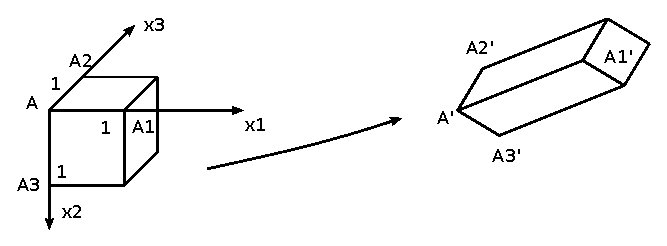
\includegraphics{../images/T1_Ch03-0003}
\end{center}
\begin{equation}
    \left\{
    \begin{aligned}
        A'A_1' &= \sqrt{1+2E_{11}}\\
        \left( A'A_1',\ A'A_2' \right) &= \arcsin \frac{2E_{12}}{\sqrt{1+2E_{11}}\sqrt{1+2E_{22}}}
    \end{aligned}
    \right.
    \label{eq:Ch03-019}
\end{equation}

Comme pour le tenseur des contraintes, on peut diagonaliser le tenseur des déformations, c'est-à-dire trouver un repère orthogonal où la matrice représentant $\mathbb{E}$ est diagonale, $E_1$, $E_2$ et $E_3$ sont appelés allongements
\begin{equation}
    \mathbb{E} = 
    \begin{bmatrix}
        E_1 & 0 & 0 \\
        0 & E_2 & 0 \\
        0 & 0 & E_3
    \end{bmatrix}
    \label{eq:Ch03-020}
\end{equation}
principaux.
La propriété caractéristique des axes principaux des déformations est que les glissements dans leur direction sont nuls.
Un cube unité d'arête dirieée selon les axes principaux se transforme en un parallélépipède rectange
\begin{center}
    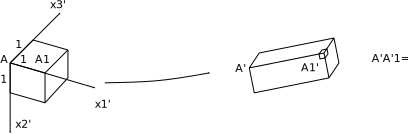
\includegraphics{../images/T1_Ch03-0004}
\end{center}

En mécanique des solides, on introduit souvent le vecteur déplacement $\vec{u} = \vec{x}-\vec{a}$, définissant le mouvement par
\begin{equation}
    x_i = a_i + u_i \left( a_1, a_2, a_3, t \right)
    \label{eq:Ch03-021}
\end{equation}
On obtient alors à partir de \eqref{eq:Ch03-022}
\begin{equation}
    F_{ij} = \delta_{ij} + \frac{\partial u_i}{\partial a_j}
    \label{eq:Ch03-022}
\end{equation}
Le tenseur des déformations est alors donné par
\begin{equation}
    E_{ij} = \frac{1}{2} \left( \frac{\partial u_i}{\partial a_j} + \frac{\partial u_j}{\partial a_i} + \frac{\partial u_k}{\partial a_i}\frac{\partial u_k}{\partial a_j} \right)
    \label{eq:Ch03-023}
\end{equation}
\section{Petites déformations} \label{sec:Ch03-2}
\subsection{Hypothèse des petites perturbations} \label{ssec:Ch03-2.1}
En Mécanique des Solides, on fait souvent l'hypothèse des petites perturbations pour laquelle le solide s'écarte peu de sa configuration de référence. Les déplacements et les déformations restent petits, ce qui a deux conséquences essentielles:
\begin{enumerate}
    \item on peut identifier variables de Lagrange $a_i$ et variables d'Euler $x_i$, dans la mesure où la différence entre les deux est négligeable.
        Ceci est tout à fait essentiel, car certaines équations s'écrivent naturellement en variables eulériennes ---les équations d'équilibre, par exemple--- alors que d'autres s'écrivent plus naturellement en variables lagrangiennes ---la définition des déformations.
        Entre autres, cela revient à écrire les équations d'équilibre dans la configuration telle qu'elle existe avant déformation, alors qu'il faudrait, en toute rigueur, les écrire dans la configuration réelle où s'appliquent effectivement les efforts.
        Cette approximation, habituellement appelée hypothèse de linéarité externe, est souvent justifiée mais on rencontrera quelques cas, en particulier toutes les questions de stabilité, où elle ne l'est pas;
    \item dans tous les calculs, on ne conserve que les termes les plus significatifs, en négligeant les termes d'ordre supérieur en $u_i$ et ses dérivées.
        En d'autres termes, on effectue une linéarisation autour de la configuration de référence, supposée naturelle, c'est-à-dire libre de contraintes, cararctérisée par 
        \begin{equation}
            \rho = \rho_c, \quad u_i = 0, \quad \sigma_{ij} = 0
            \label{eq:Ch03-024}
        \end{equation}
        et le mouvement est décrit par
        \begin{equation}
            \rho = \rho_0 + \rho, \quad u_i, \quad \sigma_{ij}
            \label{eq:Ch03-025}
        \end{equation}
        avec $\rho'$, $u_i$, $\sigma_{ij}$ petits et fonctions de $\left( x_i,t \right)$, $x_i$ représentant indifféremment les variables de Lagrange $a_i$ ou d'Euler $x_i$.
        La vitesse $V_i$ et l'accélération $\gamma_i$ sont données par
        \begin{equation}
            V_i = \frac{\partial u_i}{\partial t}, \quad \gamma_i = \frac{\partial^2 u_i}{\partial t^2}
            \label{eq:Ch03-026}
        \end{equation}
        en remarquant que les dérivées particulaires sont des dérivées partielles par rapport au temps en variables de Lagrange.
        L'équation de continuité~\eqref{eq:Ch01-011} donne
        \begin{equation*}
            \frac{\ud}{\ud t} \left( \rho_0 +\rho' \right) + \left( \rho_0 + \rho' \right) \frac{\partial V_i}{\partial x_i} = 0
        \end{equation*}
        mais  $\ud \rho_0/\ud t$, $\ud \rho' / \ud t = \partial \rho' / \partial t$ en variables de Lagrange, et on peut négliger le  terme $\rho' \partial V_i / \partial x_i$ qui est du second ordre par rapport à la perturbation.
        Il  reste  donc
        \begin{equation*}
            \frac{\partial \rho'}{\partial t} + \rho_0' \frac{\partial^2 u_i}{\partial x_i \partial t} = 0
        \end{equation*}
        ou en intégrant par rapport au temps
        \begin{equation}
            \rho' = - \rho_0 \frac{\partial u_i}{\partial x_i}
            \label{eq:Ch03-027}
        \end{equation}
        la constante d'intégration étant nulle puisque dans la configuration de référence $\rho'$ et $u_i$ sont nuls.
        Nous retrouverons cette relation au paragraphe~\ref{ssec:Ch03-2.2}.
        De même, 1'équation du mouvement \eqref{eq:Ch01-015} donne
        \begin{equation}
            \rho_0 \frac{\partial^2 u_i}{\partial t^2} = \frac{\partial \sigma_{ij}}{\partial x_j} + f_i
            \label{eq:Ch03-028}
        \end{equation}
\end{enumerate}
En particulier, on constate que $\rho'$ disparaît disparaît de l'équation du mouvement.
En Mécanique des Solides, on peut oublier l'équation de continuité qui permet seulement de calculer $\rho'$ par \eqref{eq:Ch03-027} une fois connu le déplacement $u_i \left( x_i, t \right)$.
\subsection{Tenseur linéarisé des déformations} \label{ssec:Ch03-2.2}
Dans le cadre d'hypothèse des petites perturbations, le tenseur des déformations introduit au paragraphe~\ref{ssec:Ch03-1.2} et défini par \eqref{eq:Ch03-023} à partir du déplacement $u_i$ devient
\begin{equation}
    \varepsilon_{ij} = \frac{1}{2} \left( \frac{\partial u_i}{\partial x_j} + \frac{\partial u_j}{\partial x_i} \right)
    \label{eq:Ch03-029}
\end{equation}
Ce tenseur $\varepsilon_{ij}$ est le tenseur des déformations linéarisées.
En grandes déformations, en effet, le tenseur de Green-Lagrange que nous avons défini, n'est pas le seul possible, et on peut en introduire bien d'autres, mais en petites déformations, tous ces tenseurs se réduisent au tenseur $\mathbb{\varepsilon}$ défini par~\eqref{eq:Ch03-029}.
Par linéarisation des formules \eqref{eq:Ch03-015} et \eqref{eq:Ch03-016}, il permet de calculer l'allongement dans une direction $\vec{n}$ le glissement dans deux directions $\vec{m}$ et $\vec{n}$ par les formules
\begin{equation}
\varepsilon (\vec{n}) = \varepsilon_{ij} n_i n_j\quad\text{et}\quad\gamma(\vec{m},\vec{n}) = 2 \varepsilon_{ij} n_i m_j \label{eq:Ch03-031} 
\end{equation}
obtenues simplement par développement limité des diverses fonctions internenant dans \eqref{eq:Ch03-015} et \eqref{eq:Ch03-016}.
On obtient aussi la signification des composantes $\varepsilon_{ij}$
\begin{equation}
    \varepsilon (\vec{e}_1) = \varepsilon_{11} = \frac{\partial u_1}{\partial x_1} \quad\text{et}\quad 
    \gamma (\vec{e}_1,\vec{e}_2) = \gamma_{12} = 2 \varepsilon_{12} = \left( \frac{\partial u_1}{\partial x_2} + \frac{\partial u_2}{\partial x_1} \right) \label{eq:Ch03-033}
\end{equation}
Pour dégager la signification de ce tenseur, on peut considérer le mouvement du voisinage d'un point $M$ on peut écrire
\begin{align*}
    \left( \overrightarrow{M'M_t'} \right)_i &= u_i \left( x + \ud x \right) \\
    &= u_i (x) + \frac{\partial u_i}{\partial x_j} (x) \ud x_j\\
    &= u_i + U_{i,j} \ud x_j
\end{align*}
On décompose alors $u_{i,j}$ en partie symétrique et antisymétrique
\begin{equation*}
    \left( \overrightarrow{M'M_t'} \right)_i = u_i + \omega_{ij} \ud x_j + \varepsilon_{ij} \ud x_j
\end{equation*}
\begin{equation}
    \varepsilon_{ij} = \frac{1}{2} \left( u_{i,j} + u_{j,i} \right), \quad \omega_{ij} = \frac{1}{2} \left( u_{i,j} - u_{j,i} \right)
    \label{eq:Ch03-034}
\end{equation}
On introduit le vecteur $\vec{\omega}$, adjoint du tenseur antimétrique $\omega_{ij}$ (Annexe~\ref{Ann:A}) par
\begin{equation}
    \omega_{ij} =
    \begin{bmatrix}
        0 & \omega_{12} & \omega_{13} \\
        \omega_{21} & 0 & \omega_{23} \\
        \omega_{31} & \omega_{32} & 0
    \end{bmatrix}
    =
    \begin{bmatrix}
        0 & -\omega_{3} & \omega_{2} \\
        \omega_{3} & 0 & -\omega_{1} \\
        -\omega_{2} & \omega_{1} & 0
    \end{bmatrix}
    \label{eq:Ch03-035}
\end{equation}
ce qui permet d'écrire pour $\omega_{ij} \ud x_j$
\begin{equation}
    \begin{bmatrix}
        0 & -\omega_{3} & \omega_{2} \\
        \omega_{3} & 0 & -\omega_{1} \\
        -\omega_{2} & \omega_{1} & 0
    \end{bmatrix}
    \begin{bmatrix}
        \ud x_1 \\
        \ud x_2 \\
        \ud x_3
    \end{bmatrix}
    =
    \begin{bmatrix}
        \omega_2 \ud x_3 - \omega_3 \ud x_2 \\
        \omega_3 \ud x_1 - \omega_1 \ud x_3 \\
        \omega_1 \ud x_2 - \omega_2 \ud x_1
    \end{bmatrix}
    \begin{bmatrix}
        \omega_1 \\
        \omega_2 \\
        \omega _3
    \end{bmatrix}
    \wedge 
    \begin{bmatrix}
        \ud x_1 \\
        \ud x_2 \\
        \ud x_3
    \end{bmatrix}
    \label{eq:Ch03-036}
\end{equation}
et finalement on a
\begin{equation}
    \overrightarrow{M'M_t'} = \underbrace{\underbrace{\vec{u}}_{\text{translation}} + \underbrace{\vec{\omega} \wedge \vec{\ud x}}_{\text{rotation}}}_{\text{mouvement rigidifiant}} + \underbrace{\mathbb{\varepsilon} \vec{\ud x}}_{\text{déformation pure}}
     \label{eq:Ch03-037}
\end{equation}
Le mouvement rotation et du voisinage d'un point $M$ se  compose  d'une  translation, d'une rotation et d'une déformation pure.

On peut refaire sur le tenseur des déformations tout ce que nous avons fait au chapitre~\ref{chap:Ch02} sur le tenseur des contraintes: diagonalisation, définition des invariants, décomposition en déviateur et partie sphérique
\begin{equation}
    \left\{
    \begin{aligned}
        \varepsilon_{ij} &= \mathbb{\varepsilon} \delta_{ij} + e_{ij} \\
        \varepsilon & = \frac{\varepsilon_{ii}}{3} = \frac{\varepsilon_{11} + \varepsilon_{22} + \varepsilon_{33}}{3} = \frac{\varepsilon_1 + \varepsilon_2 + \varepsilon_3}{3} \\
        e_{ij} &= \varepsilon_{ij} - \frac{1}{3} \varepsilon_{kk} \delta_{ij}, \quad e_{ii} = 0
    \end{aligned}
    \right.
    \label{eq:Ch03-038}
\end{equation}
Physiquement, cette décomposition correspond à la décomposition de la déformation en une dilatation uniforme (partie sphérique) et une distorsion, c'est-à-dire une déformation sans changement de volume (déviateur).
En effet, on vérifie facilement que la trace $\varepsilon_{ii}$ du tenseur des déformations est égale à la variation relative de volume
\begin{equation}
    \frac{\Delta V}{V} = \varepsilon_{ii} = 3\varepsilon
    \label{eq:Ch03-039}
\end{equation}
Il suffit par exemple de partir d'un élément de volume parallélépipédique orienté selon les directions principales du tenseur des déformations

Après déformation, cet élément devient un parallélépipède rectangle de côté $(1+\varepsilon_1)\ud x_1$, $(1+\varepsilon_2)\ud x_2$, $(1+\varepsilon_3)\ud x_3$ et son volume est
\begin{equation}
    V+\Delta V = (1+\varepsilon_1)(1+\varepsilon_2)(1+\varepsilon_3)\ud x_1 \ud x_2 \ud x_3 = \left[ 1 + \left( \varepsilon_1 + \varepsilon_2 + \varepsilon_3 \right) \right] V
\end{equation}
en négligeant les termes d'ordre 2 en $\varepsilon_1$, $\varepsilon_2$, $\varepsilon_3$, ce qui donne directement \eqref{eq:Ch03-039}.
La conservation de la masse
\begin{equation*}
    \left( \rho_0 + \rho' \right) \left( V + \Delta V \right) = \rho_0 V
\end{equation*}
donne alors
\begin{equation}
    \frac{\rho'}{\rho_0} = - \frac{\Delta V}{V} = - \varepsilon_{ii} = - u_{i,i}
    \label{eq:Ch03-040}
\end{equation}
et on retrouve \eqref{eq:Ch03-027}.
Nous terminons ce paragraphe par quelques exemples de déformatjons homogènes.
\begin{enumerate}
    \item Dilatation uniforme
        \begin{equation}
            \left\{
            \begin{aligned}
                u_i &= \alpha x_i \\
                \varepsilon_{ij} &= u_{i,j} = \alpha \delta_{ij}, \quad \frac{\Delta V}{V} = 3\alpha
            \end{aligned}
            \right.
            \label{eq:Ch03-041}
        \end{equation}
    \item Extension simple
        \begin{equation}
            \left\{
            \begin{aligned}
                u_1 &= \alpha x_1 \\
                u_2 &= -\beta x_2 \\
                u_3 &= -\beta x_3
            \end{aligned}
            \right. \qquad
            \mathbb{\varepsilon} = 
            \begin{bmatrix}
                \alpha & 0 & 0 \\
                0 & -\beta & 0 \\
                0 & 0 & -\beta
            \end{bmatrix}
            \label{eq:Ch03-042}
        \end{equation}
        Si cette extension se fait sans changement de volume, alors d'après \eqref{eq:Ch03-039}, on a $\beta = \frac{\alpha}{2}$.
        La décomposition en déviateur et partie sphérique s'écrit comme en \eqref{eq:Ch01-019}
        \begin{equation}
            \mathbb{\varepsilon} = \varepsilon 
            \begin{bmatrix}
                1 & 0 & 0 \\
                0 & 1 & 0 \\
                0 & 0 & 1
            \end{bmatrix}
            + e 
            \begin{bmatrix}
                1 & 0 & 0 \\
                0 & -\frac{1}{2} & 0 \\
                0 & 0 & -\frac{1}{2}
            \end{bmatrix}
            , \quad e \frac{2 \left( \alpha - \beta \right)}{3}
            \label{eq:Ch03-043}
        \end{equation}
    \item Glissement simple
        \begin{equation}
            \left\{
            \begin{aligned}
                u_1 &= \gamma x_1 \\
                u_2 &= 0 \\
                u_3 &= 0
            \end{aligned}
            \right. \qquad
            u_{i,j}' = 
            \begin{bmatrix}
                0 & \gamma & 0 \\
                0 & 0 & 0 \\
                0 & 0 & 0
            \end{bmatrix}
            \label{eq:Ch03-044}
        \end{equation}
        \begin{equation}
            \mathbb{\varepsilon} = 
            \begin{bmatrix}
                0 & \frac{\gamma}{2} & 0 \\
                \frac{\gamma}{2} & 0 & 0 \\
                0 & 0 & 0
            \end{bmatrix}, \quad
            \mathbb{\omega} = 
            \begin{bmatrix}
                0 & \frac{\gamma}{2} & 0 \\
                -\frac{\gamma}{2} & 0 & 0 \\
                0 & 0 & 0
            \end{bmatrix}, \quad
            \vec{\omega} = 
            \begin{bmatrix}
                0 \\
                0 \\
                \frac{-\gamma}{2}
            \end{bmatrix}
            \label{eq:Ch03-045}
        \end{equation}
        Le mouvement se compose de la déformation définie par $\varepsilon$ et d'une rotation de $\frac{-\gamma}{2}$ autour de l'axe $x_3$.

        Pour visualiser les déformations, on a représenté des déformations importantes, mais il ne faut pas oublier que les déformations sont en fait petites: $\alpha$, $\beta$, $\gamma$ sont des quantités petites.
\end{enumerate}
\subsection{Dualité contraintes--déformations} \label{ssec:Ch03-2.3}
On remarque l'analogie entre le tenseur des déformations $\varepsilon_{ij}$, défini par \eqref{eq:Ch03-029} à partir du déplacement $u_i$ et le tenseur des taux de déformations $D_{ij}$ défini par \eqref{eq:Ch01-023} à partir des vitesses $V_i$.
Tout ce que nous avons fait au paragraphe~\ref{ssec:Ch03-2.2} sur le petit déplacement $u_i$, en particulier toutes les interprétations physiques, peut se transposer directement aux vitesses $V_i$ qui représentent le déplacement infinitésimal entre la configuration à l'instant $t$ et celle à l'instant $t+\ud t$.
Plus précisément, on a l'analogie suivante
\begin{center}
    \begin{tabular}[c]{lccr}
        Déplacements & $u_i$ & $V_i$ & Vitesses \\
        gradient des déplacements & $u_{i,j}$ & $V_{i,j}$ & gradient des vitesses \\
        tenseur des déformations & $\varepsilon_{ij}$ & $D_{ij}$ & tenseur des taux de déformation \\
        tenseur des rotations & $\omega_{ij}$ & $\Omega_{ij}$ & tenseur taux de rotation \\
        vecteur rotation & $\vec{\omega}$ & $\vec{\Omega}$ & vecteur taux de rotation \\
        allongement dans la direction $\vec{n}$ & $\varepsilon (\vec{n})$ & & taux d'allongement \\
        glissement dans les directions $\vec{m}$, $\vec{n}$ & $\gamma (\vec{m},\vec{n})$ & & taux de glissement \\
        etc.
    \end{tabular}
\end{center}

Réciproquement, tout ce que nous avons fait au paragraphe~\ref{ssec:Ch03-1.2} peut se transposer directement en termes de déplacements.
Il s'agit simplement d'un changement de terminologie.
On parle de déplacement virtuel ${\mathop{u}^{*}}_i$ au lieu de vitesses virtuelles ${\mathop{V}^{*}}_i$ et de \emph{travaux virtuels} au lieu de \emph{puissances virtuelles}.
Par exemple, \eqref{eq:Ch01-024} ou \eqref{eq:Ch01-038} peut s'écrire
\begin{equation}
    \iiint_{\Omega} \rho \gamma_i {\mathop{u}^*}_i \ud v = \iiint_{\Omega} f_i {\mathop{u}^*}_i \ud v + \iint_{\partial \Omega} T_i {\mathop{u}^*}_i \ud S - \iiint_{\Omega} \sigma_{ij} {\mathop{\varepsilon}^*}_{ij} \ud v
    \label{eq:Ch03-046}
\end{equation}
expression du théorème des travaux virtuels ou du principe des travaux virtuels, suivant le point de vue que l'on adopte.

En particulier, le travail des efforts intérieurs par unité de volume est
\begin{equation}
    {\mathop{w}^*}_{int} = \sigma_{ij} {\mathop{\varepsilon}^*}_{ij}
    \label{eq:Ch03-047}
\end{equation}
qui met en dualité le tenseur des contraintes $\sigma_{ij}$ que nous avons étudié au chapitre~\ref{chap:Ch02}, et le tenseur des déformations $\varepsilon_{ij}$ que nous venons d'introduire.
C'est une propriété tout à fait universelle: dans toute théorie des milieux continus, il y a dualité entre les contraintes et les déformations, c'est-à-dire entre la schématisation des efforts intérieurs et la description cinématique.

Dans le cadre de la MMC classique, que nous développons actuellement, cela n'apporte qu'une simple vérification.
Dans d'autres cas, où la schématisation à adopter est moins évidente, cela sera pour nous un guide précieux.

On peut pousser plus loin cette dualité, en remarquant que dans toute théorie des milieux continus, on travaille sur quatre espaces:
\begin{itemize}
    \item l'espace des déplacements, $\mathcal{U}$,  $u \in \mathcal{U}$
    \item l'espace des déformations, $\mathcal{D}$, $\varepsilon \in \mathcal{D}$
    \item l'espace des contraintes, $\mathcal{S}$,  $\sigma \in \mathcal{S}$
    \item l'espace des chargements, $\mathcal{C}$, $\phi = \left( f_i, T_i^e \right) \in \mathcal{C}$
\end{itemize}
Le travail des efforts extérieurs met en dualité $\mathcal{U}$ et $\mathcal{C}$ par
\begin{equation}
    \langle u, \phi \rangle = \iiint_{\Omega} u_i f_i \ud v + \iint_{\partial \Omega} u_{i} T_i^e \ud S
    \label{eq:Ch03-048}
\end{equation}
Le travail des efforts intérieurs met en dualité $\mathcal{D}$ et $\mathcal{S}$ par
\begin{equation}
    \langle\langle \varepsilon, \sigma \rangle\rangle = \iiint_{\Omega} \sigma_{ij} \varepsilon_{ij} \ud v
    \label{eq:Ch03-049}
\end{equation}
et, en statique, le théorème des travaux virtuels \eqref{eq:Ch03-046} peut s'écrire
\begin{equation}
    \langle\langle \mathop{\varepsilon}^* , \sigma \rangle \rangle = \langle \mathop{u}^* , \phi \rangle
    \label{eq:Ch03-050}
\end{equation}
Nous reviendrons sur cette dualité lorsque nous parlerons des méthodes variationnelles auchapitre \ref{chap:Ch09}.
\section{Compatibilite des déformations} \label{sec:Ch03-3}
Connaissant le champ des déplacements $u_i (x)$, on en déduit par~\eqref{eq:Ch03-029}, le champ des déformations $\varepsilon_{ij}(x)$.
Réciproquement, si on connaît le champ des déformations $\varepsilon_{ij}(x)$, peut-on calculer le champ des déplacements $u_i (x)$ ? Et si oui, comment?

Le premier problème est celui de la compatibilité des déformations, le second celui de l'intégration d'un champ de déplacements.
Ce problème est extrêmement important en mécanique des solides, car nous verrons que la solution s'obtient souvent sous forme d'un champ de déformation; il faut alors remonter aux déplacements.
Remarquons que, en vertu de l'analogie discutée au paragraphe~\ref{ssec:Ch03-2.3}, on pourra transposer tous nos résultats en termes de vitesse et de taux de déformation, le problème étant alors de calculer le champ des vitesses à partir de la valeur en tout point du tenseur taux de déformation.
\subsection{Calcul de la rotation} \label{ssec:Ch03-3.1}
Pour calculer le déplacement $u_i$, il faut intégrer les formes différentielles 
\begin{equation}
    \ud u_i = u_{i,j} \ud x_j = \left( \varepsilon_{ij} + \omega_{ij} \right) \ud x_j
    \label{eq:Ch03-051}
\end{equation}
Or, on connaît $\varepsilon_{ij}(x)$ mais on ne connaît pas $\omega_{ij}$.
La première étape consiste donc à calculer la rotation $\omega_{ij}$.
\begin{lem} \label{lem:Ch03-1}
    Les dérivées de la rotation sont liées à celles de la déformation par la relation
    \begin{equation}
        \omega_{ij,l} = \varepsilon_{il,j} - \varepsilon_{jl,i}
        \label{eq:Ch03-052}
    \end{equation}
\end{lem}
\begin{proof}
    On part de la définition 
    \begin{align*}
        \omega_{ij} &= \frac{1}{2} \left( u_{i,j} - u_{j,i} \right) = \frac{1}{2} \left( u_{i,jl} - u_{j,il} \right) = \frac{1}{2} \left( u_{i,jl} + u_{l,ij} - u_{l,ij} - u_{j,il} \right) \\
        &= \frac{1}{2} \left( u_{i,l} + u_{l,i} \right)_{,j} - \frac{1}{2} \left( u_{l,j} + u_{j,l} \right)_{,i} \\
        &= \varepsilon_{il,j} - \varepsilon_{jl,i}
    \end{align*}
    en utilisant le fait que les dérivées partielles commutent: $u_{i,jl} = u_{i,lj}$, etc.
\end{proof}

On peut alors calculer la rotation $\omega_{ij}$ par intégration du système
\begin{equation}
    \ud \omega_{ij} = \left( \varepsilon_{il,j} - \varepsilon_{jl,i} \right) \ud x_l
    \label{eq:Ch03-053}
\end{equation}
\begin{lem} \label{lem:Ch03-2}
    Une condition nécessaire et suffisante pour que le système 
    \begin{equation}
        \ud f = a_l \ud x_l
        \label{eq:Ch03-054}
    \end{equation}
    soit intégrable, c'est-à-dire pour que l'on puisse calculer $f$ à partir des $a_l = f_{,l}$ est que 
    \begin{equation}
        a_{l,m} = a_{m,l}
        \label{eq:Ch03-055}
    \end{equation}
\end{lem}
\begin{proof}
    La condition nécessaire est évidente (elle exprime simplement que $f_{,lm} = f_{,ml}$).
    On démontre en mathématiques que cette condition est également suffisante.
\end{proof}

En appliquant ce lemme au système différentiel~\eqref{eq:Ch03-053}, on obtient la condition suivante
\begin{equation}
        \left( \varepsilon_{il,j} -\varepsilon_{jl,i} \right)_{,k} = \left( \varepsilon_{ik,j} - \varepsilon_{jk,i} \right)_{,l} \quad\Leftrightarrow\quad
        \varepsilon_{il,jk} + \varepsilon_{jk,il} - \varepsilon_{jl,ik} - \varepsilon_{ik,jl} = 0
    \label{eq:Ch03-056}
\end{equation}
Cette condition est une condition nécessaire et suffisante pour que l'on puisse calculer $\omega_{ij}$ à partir de $\varepsilon_{ij}$.
C'est donc une condition nécessaire pour que le champ de déformation $\varepsilon_{ij}$ soit intégrable, c'est-à-dire pour que l'on puisse calculer le déplacement $u_i$.

On tire également du Lemme~\ref{lem:Ch03-1} le résultat suivant
\begin{thm} \label{thm:Ch03-2}
    Si le champ de déformation est identiquement nul, alors le déplacement est un déplacement de solide rigide 
    \begin{equation}
        \vec{u} = \vec{c} + \vec{\omega} \wedge \vec{x}
        \label{eq:Ch03-057}
    \end{equation}
\end{thm}
Il est en effet clair que si le déplacement est un déplacement de solide rigide, infinitésimal, bien entendu, alors le tenseur des déformations associé est nul, puisque $u_{i,j}$ est antisymétrique.
Le théorème~\ref{thm:Ch03-2} constitue une réciproque.
Compte-tenu de l'analogie présentée au paragraphe~\ref{ssec:Ch03-2.3}, ce théorème est identique au Lemme~\ref{lem:Ch01-3} paragraphe~\ref{ssec:Ch01-2.1}.

\begin{proof}
    Puisque $\varepsilon_{ij}$ est nul, le Lemme~\ref{lem:Ch03-1} montre que $\omega_{ij,l}$ est nul, et donc que $\omega_{ij}$ est constant
    \begin{equation*}
        u_{i,j} = \not{\varepsilon_{ij}} + \omega_{ij} = \omega_{ij}^0
    \end{equation*}
    Le système~\eqref{eq:Ch03-051} s'intègre alors directement pour donner
    \begin{equation*}
        u_i = \omega_{ij}^0 x_j + c_{j}^0
    \end{equation*}
    que l'on peut écrire sous la forme \eqref{eq:Ch03-057} en introduisant le vecteur $\vec{\omega}$ adjoint du tenseur antisymétrique $\omega_{ij}^0$ (le calcul est le même que celui qui a conduit à \eqref{eq:Ch03-037}.
\end{proof}
\subsection{Calcul du déplacement} \label{ssec:Ch03-3.2}
Sous réserve que la condition~\eqref{eq:Ch03-056} soit vérifiée, l'intégration du système \eqref{eq:Ch03-053} donne $\omega_{ij}$ à une constante près $\omega_{ij}^0$.
Le déplacement $u_i$ s'obtiendra alors en intégrant le système \eqref{eq:Ch03-051}
\begin{equation*}
    \ud u_i = u_{i,j} \ud x_j = \left( \varepsilon_{ij} + \omega_{ij} \right) \ud x_j
\end{equation*}
Pour que cela soit possible, il faut et il suffit, d'après le Lemme~\ref{lem:Ch03-2}, que
\begin{equation*}
    \varepsilon_{ij,l} + \omega_{ij,l} = \varepsilon_{il,j} + \omega_{il,j}
\end{equation*}
Cependant, les dérivées $\omega_{ij,l}$ ont été calculées par \eqref{eq:Ch03-052}, et cette condition devient 
\begin{equation*}
    \varepsilon_{ij,l} + \varepsilon_{il,j} - \varepsilon_{jl,i} = \varepsilon_{il,j} + \varepsilon_{ij,l} - \varepsilon_{jl,i}
\end{equation*}
condition qui se trouve identiquement vérifiée, et le système \eqref{eq:Ch03-051} peut toujours s'intégrer à un déplacement de la forme 
\begin{equation*}
    \omega_{ij}^0 x_j + c_i^0
\end{equation*}
près, c'est-à-dire à un déplacement de solide rigide près.
Nous avons donc démontré le résultat suivant
\begin{thm} \label{thm:Ch03-3}
    Pour que le champ de déformation $\varepsilon_{ij}(x)$ soit intégrable, il faut et il suffit que les \emph{équations de compatibilité}~\eqref{eq:Ch03-056}
    \begin{equation*}
        \varepsilon_{il,jk} + \varepsilon_{jk,il} - \varepsilon_{jl,ik} - \varepsilon_{ik,jl} = 0
    \end{equation*}
    soient vérifiées.
    On peut alors calculer le déplacernent à un déplacement de solide près.
\end{thm}

Pratiquement, pour intégrer un champ de déformation $\varepsilon_{ij}$, c'est-à-dire pour calculer $u_i$ par résolution du système d'équations aux dérivées partielles 
\begin{equation}
    \frac{\partial u_i}{\partial x_j} + \frac{\partial u_j}{\partial x_i} = \varepsilon_{ij} (x)
    \label{eq:Ch03-058}
\end{equation}
il faut vérifier les équations de compatibilité~\eqref{eq:Ch03-056}; si elles ne sont pas vérifiées, le problème n'admet pas de solution. Si elles le sont, alors on peut  calculer le déplacement $u_i$; pour cela, on peut utiliser deux méthodes:
\begin{enumerate}
    \item méthode systématique: on intègre~\eqref{eq:Ch03-053}, puis \eqref{eq:Ch03-051};
    \item méthode directe: on calcule par résolution directe de \eqref{eq:Ch03-058} une solution particulière, et on remarque que la solution générale de \eqref{eq:Ch03-058} est la somme d'une solution particulière et de la solution générale de l'équation sans second membre, $\varepsilon_{ij} = 0$, qui, d'après le Théorème~\ref{thm:Ch03-2}, est un déplacement de solide rigide.
        Nous verrons dans la suite des exemples de cette démarche.
\end{enumerate}
Les équations de compatibilité \eqref{eq:Ch03-056} font intervenir quatre indices $i$, $j$, $k$ et $l$, variant de 1 à 3, soit \textit{a priori} 81 équations. Néanmoins, on constate que la quantité \eqref{eq:Ch03-056} est antisymétrique en $i$ et $j$, antisymétrique en $k$ et $l$, et symétrique par rapport aux couples $(i,j)$ et $(k,l)$.
Il reste donc finalement six équations indépendantes obtenues pour $ijkl = (1212),\ (1213)$, et permutation circulaire. On obtient
\begin{equation}
        \varepsilon_{11,22} + \varepsilon_{22,11} - 2 \varepsilon_{12,12} = 0 \quad\text{et}\quad
        \varepsilon_{11,23} + \left( \varepsilon_{23,1} - \varepsilon_{31,2} - \varepsilon_{12,3} \right)_{,1} = 0
    \label{eq:Ch03-059}
\end{equation}
et les qutre équations qui s'en déduisent par permutation circulaire.
On peut également obtenir un système de six équations équivalentes, en faisant $k=j$
\begin{equation}
    \begin{aligned}
        &\varepsilon_{il,kk} + \varepsilon_{kk,il} - \left( \varepsilon_{kl,ik} + \varepsilon_{ik,kl} \right) = 0 \\
        &\Delta\varepsilon_{ij} + \varepsilon_{kk,ij} - \left( \varepsilon_{jk,ik} + \varepsilon_{ik,jk} \right) = 0
    \end{aligned}
    \label{eq:Ch03-060}
\end{equation}
forme symétrique en $i,j$, qui donne donc 6 équations équivalentes à \eqref{eq:Ch03-059}.

Terminons par deux cas particuliers importants.
\begin{enumerate}
    \item Déformation homogène
        \begin{equation}
            \varepsilon_{i?} = \varepsilon_{ij}^0 = \text{Cte}
            \label{eq:Ch03-061}
        \end{equation}
        En intégrant \eqref{eq:Ch03-053}, il vient $\omega_{ij} = \omega_{ij}^0 = \text{Cte}$ et \eqref{eq:Ch03-051} donne
        \begin{equation}
            \vec{u} = \mathbb{\varepsilon}^0 \vec{x} + \vec{\omega} \wedge \vec{x} + \vec{c}
            \label{eq:Ch03-062}
        \end{equation}
    \item Déformation linéaire
        \begin{equation}
            \varepsilon_{ij} = A_{ijk} x_k
            \label{eq:Ch03-063}
        \end{equation}
        forme qui fait intervenir 18 coefficients $A_{ijk} = A_{jik}$.
        Les équations de compatibilité \eqref{eq:Ch03-059}, ne faisant intervenir que des derivées secondes de $\varepsilon_{ij}$ sont automatiquement vérifiées.
        Par intégration de \eqref{eq:Ch03-053} et \eqref{eq:Ch03-051}, on trouve
        \begin{equation}
            \begin{aligned}
                \ud \omega_{ij} &= \left( A_{ikj} - A_{jki} \right) \ud x_k \\
                \omega_{ij} &= \left( A_{ikj} - A_{jki} \right) x_k + \omega_{ij}^0
            \end{aligned}
            \label{eq:Ch03-064}
        \end{equation}
et:
        \begin{equation}
            \begin{aligned}
                \ud u_i &= \left( A_{ijk} + A_{ikj} - A_{jki} \right) x_k \ud x_j + \omega_{ij}^0 \ud x_j \\
                u_i &= \frac{1}{2} \left( A_{ijk} + A_{ikj} - A_{jki} \right) x_j x_k + \omega_{ij}^0 x_j + c_i^0
            \end{aligned}
            \label{eq:Ch03-065}
        \end{equation}
\end{enumerate}

\appendix
\chapter{Notations tensorielles} \label{Ann:A}
L'objectif de cette annexe est de familiariser le lecteur avec les notations tensorielles.
Les résultats que nous démontrerons sont tout à fait classiques et il convient de les considérer comme des exercices pour l'apprentissage des manipulations indicielles.
\section{Vecteurs et tenseurs}
\subsection{Notations indicielles}
Nous nous plaçons dans l'espace l'euclidien $E$ à trois dimensions.
Soit $(\vec{e}_1,\vec{e}_2,\vec{e}_3)$ une base orthonormée.
Un vecteur $\vec{V}$ est alors représenté par ses composantes $V_1$, $V_2$ et $V_3$:
\begin{equation}
    \vec{V} = V_1 \vec{e}_1 + V_2 \vec{e}_2 + V_3 \vec{e}_3 = V_i \vec{e}_i
    \label{eq:AnnA-001}
\end{equation}
en utilisant la convention de sommation: chaque fois que dans une expression un indice est répété, il convient de faire varier cet indice de 1 à 3 et de faire la somme.
Dans l'expression~\eqref{eq:AnnA-001}, l'indice $i$ est \emph{muet}: on aurait aussi bien pu écrire $V_j \vec{e}_j$ ou $V_k \vec{e}_k$.

Soit $\mathbb{A}$ une application linéaire, alors dans la base $(\vec{e}_1,\vec{e}_2,\vec{e}_3)$, cette application est représentée par une matrice $3\times3$:
\begin{equation}
    \mathbb{A} \text{ repr } 
    \begin{bmatrix}
        A_{11} & A_{12} & A_{13} \\    
        A_{21} & A_{22} & A_{23} \\    
        A_{31} & A_{32} & A_{33} 
    \end{bmatrix}
    \label{eq:AnnA-002}
\end{equation}
et, si $\vec{W} = \mathbb{A} \vec{V}$, les composantes de $\vec{W}$ sont données par:
\begin{align*}
    W_1 &= A_{11} V_1 + A_{12} V_2 + A_{13} V_3\\
    W_2 &= A_{21} V_1 + A_{22} V_2 + A_{23} V_3\\
    W_3 &= A_{31} V_1 + A_{32} V_2 + A_{33} V_3
\end{align*}
que nous pouvons condenser en:
\begin{equation}
    W_i = A_{ij} V_j
    \label{eq:AnnA-003}
\end{equation}
L'indice $j$ est un indice muet: on aurait aussi bien pu écrire $A_{ik} V_k$.
L' indice $i$ est un indice \emph{libre}.
Dans une égalité, on doit avoir pour chaque terme les mêmes indices libres.

Nous introduisons les symboles de Kronecker:
\begin{equation}
    \delta_{ij} = 
    \begin{cases} 
        1 & \text{ si } i = j\\
        0 & \text{ si } i \neq j
    \end{cases}
    \label{eq:AnnA-004}
\end{equation}
En particulier, l'application identité $\mathbb{I}$ est représentée par la matrice de composantes $\delta_{ij}$:
\begin{displaymath}
    \mathbb{I} \text{ repr } 
    \begin{bmatrix}
        \delta_{11} & \delta_{12} & \delta_{13} \\
        \delta_{12} & \delta_{22} & \delta_{23} \\
        \delta_{31} & \delta_{32} & \delta_{33} 
    \end{bmatrix}
    =
    \begin{bmatrix}
        1 & 0 & 0 \\
        0 & 1 & 0 \\
        0 & 0 & 1
    \end{bmatrix}
\end{displaymath}
Si la base $(\vec{e}_1,\vec{e}_2,\vec{e}_3)$ est orthonormée, alors:
\begin{equation}
    \vec{e}_i \cdot \vec{e}_j = \delta_{ij}
    \label{eq:AnnA-005}
\end{equation}
et le produit scalaire de deux vecteurs est:
\begin{equation}
        \vec{V} \cdot \vec{W} = V_i \vec{e}_i \cdot W_j \vec{e}_j = V_i W_j \vec{e}_i \cdot \vec{e}_j
         = V_i W_j \delta_{ij}  =V_i W_i
    \label{eq:AnnA-006}
\end{equation}
De même, la composition de deux applications linéaires se traduît par le produit de leurs matrices représentatives, c'est-à-dire en notations indicielles:
\begin{equation}
    \mathbb{C} = \mathbb{A} \circ \mathbb{B}, \quad C_{ik} = A_{ij} B_{jk}
    \label{eq:AnnA-007}
\end{equation}
\subsection{Changement de repère}
Soit $(\vec{e}_i)$ une base orthonormée et $(\vec{e}_i{}')$ une autre base orthonormée.
Soit $Q_{ij}$ la matrice de passage:
\begin{equation}
\begin{aligned}
    \vec{e}_1{}' &= Q_{11} \vec{e}_1 + Q_{12} \vec{e}_2 + Q_{13} \vec{e}_3 \\
    \vec{e}_2{}' &= Q_{21} \vec{e}_1 + Q_{22} \vec{e}_2 + Q_{23} \vec{e}_3 \\
    \vec{e}_3{}' &= Q_{31} \vec{e}_1 + Q_{32} \vec{e}_2 + Q_{33} \vec{e}_3 
\end{aligned}\quad \Leftrightarrow\quad
    \vec{e}_i{}' = Q_{ij} \vec{e}_j
    \label{eq:AnnA-008}
\end{equation}
Les deux bases étant orthonormées, on doit avoir:
\begin{equation}
    \delta_{ij} = \vec{e}_i{}' \cdot \vec{e}_j{}' = Q_{ik} Q_{jl} \vec{e}_k \cdot \vec{e}_l = Q_{ik} Q_{jk}
\end{equation}
qui montre que la matrice inverse de $Q_{ij}$ est la matrice transposée:
\begin{equation}
    Q_{ik}Q_{jk} = Q_{ki} Q_{kj} = \delta_{ij}
    \label{eq:AnnA-009}
\end{equation}
En particulier, on déduit de \eqref{eq:AnnA-008}, la relation inverse:
\begin{equation}
    \vec{e}_j = Q_{kj} \vec{e}_k{}'
    \label{eq:AnnA-010}
\end{equation}
qui s'obtient par le calcul suivant: on multiplie \eqref{eq:AnnA-008} par $Q_{ik}$ et on utilise \eqref{eq:AnnA-009}:
\begin{equation}
    Q_{ik} \vec{e}_i{}' = Q_{ik} Q_{ij} \vec{e}_j = \delta_{kj} \vec{e}_j = \vec{e}_k
\end{equation}
c'est-à-dire \eqref{eq:AnnA-010} à un changement d'indices près.
\subsection{Vecteurs}
Soit $\vec{V}$ un vecteur, $V_i$ ses composantes dans la base $\vec{e}_i$ et $V_i'$ celles dans la base $\vec{e}_i{}'$:
\begin{equation}
    \vec{V} = V_i \vec{e}_i = V_i' \vec{e}_i{}'
    \label{eq:AnnA-011}
\end{equation}
Pour obtenir 1es lois de transformation permettant de passer de nous utilisons \eqref{eq:AnnA-010}:
\begin{displaymath}
    \vec{V} = V_i \vec{e}_i = V_i Q_{ki} \vec{e}_k{}'
\end{displaymath}
et par identification avec~\eqref{eq:AnnA-011}, il vient:
\begin{equation}
    V_k' = Q_{ki} V_i, \quad V_j =  Q_{ij} V_i'
    \label{eq:AnnA-012}
\end{equation}
formule de transformation des composantes d'un vecteur.

On appelle \emph{invariant} une fonction des composantes d'un ou plusieurs vecteurs indépendante du repère choisi.
Par exemple, l'invariant produit scalaire est défini par:
\begin{equation}
    \vec{V}\cdot \vec{W} = V_i W_i
    \label{eq:AnnA-013}
\end{equation}
C'est un invariant car, d'après \eqref{eq:AnnA-012} et \eqref{eq:AnnA-009}:
\begin{displaymath}
    V_i' W_i' = Q_{ij} V_j Q_{ik} W_k = \delta_{jk} V_j W_k = V_j W_j
\end{displaymath}
\subsection{Applications linéaires}
Soit $\mathbb{A}$ une application linéaire de $E$ dans $E$. 
Dans la base $\vec{e}_i$, elle est représentée par une matrice $A_{ij}$ et dans la base $\vec{e}_i{}'$, par une autre matrice $A_{ij}'$.
Pour obtenir les lois de transformation, nous partons de \eqref{eq:AnnA-003} et de \eqref{eq:AnnA-012}:
\begin{equation}
    W_i = A_{ij} V_j, \quad W_i' = A_{ij}' V_j',\quad
    W_i' = Q_{ik} W_k = Q_{ik} A_{kl} V_l = Q_{ik} A_{kl} Q_{jl} V_{j}'
\end{equation}
et par identification, il vient:
\begin{equation}
    A_{ij}' = Q_{ik} Q_{jl} A_{kl}, \quad A_{ij} = Q_{ki} Q_{lj} A_{kl}'
    \label{eq:AnnA-014}
\end{equation}
En particulier, on a vu que les symboles de Kronecker $\delta_{ij}$ étaient les composantes de la matrice associée à l'application identité. 
Par application de \eqref{eq:AnnA-014}:
\begin{equation}
    \delta_{ij}' = Q_{ik} Q_{jl} \delta_{kl} = Q_{ik} Q_{jk} = \delta_{ij}
    \label{eq:AnnA-015}
\end{equation}
et l'application identité est représentée dans toute base par la même matrice.
\subsection{Formes bilinéaires}
Soit $A$ une forme bilinéaire sur $E$, c'est-à-dire une application bilinéaire $E\times E \rightarrow \mathbb{R}$.
Dans une base $\vec{e}_i$, elle est représentée par une matrice $A_{ij}$ telle que:
\begin{equation}
    A \bigl( \vec{V}, \vec{W} \bigr) = A_{ij} V_i W_j
    \label{eq:AnnA-016}
\end{equation}
Pour obtenir la loi de transformation de $A_{ij}$ nous partons de \eqref{eq:AnnA-016} et de \eqref{eq:AnnA-012}:
\begin{equation}
    A\bigl( \vec{V}, \vec{W} \bigr) = A_{ij} V_i W_j = A_{ij}' V_i'W_j'
    = A_{ij} Q_{ki} V_k' Q_{lj} W_l'
    \label{eq:AnnA-017}
\end{equation}
d'où par identification:
\begin{equation}
    A_{ij}' = Q_{ik} Q_{jl} A_{kl}, \quad A_{ij} = Q_{ki} Q_{lj} A_{kl}'
    \label{eq:AnnA-018}
\end{equation}
c'est-à-dire la même loi de transformation que pour une application linéaire.
Ceci est évidemment dû au fait que nous n'envisageons que des repères orthonormés.
En particulier, la forme bilinéaire représentée dans toute base par les symboles de Kronecker est le produit scalaire.
\subsection{Tenseurs du second ordre}
Il résulte de ce qui précède que l'on peut identifier application linéaire et forme bilinéaire sur $E$.
Nous appellerons \emph{tenseur du second ordre}, cette entité mathématique, généralisation de la notion de vecteur.
Algébriquement, on peut la définir en introduisant une opération bilinéaire \emph{produit tensoriel}, notée $\otimes$, et le tenseur $\mathbb{A}$ sera défini à partir de ses composantes $A_{ij}$ par:
\begin{equation}
    \mathbb{A} = A_{ij} \vec{e}_i \otimes \vec{e}_j
    \label{eq:AnnA-019}
\end{equation}
formule qui généralise~\eqref{eq:AnnA-001}.
On obtient alors directement la loi de transformation~\eqref{eq:AnnA-014} ou \eqref{eq:AnnA-018} à partir de \eqref{eq:AnnA-008} ou \eqref{eq:AnnA-010}:
\begin{equation}
    \mathbb{A} = A_{ij} \vec{e}_i \otimes \vec{e}_j = A_{ij}' \vec{e}_i{}' \otimes \vec{e}_j{}'= A_{ij} Q_{ki} \vec{e}_k{}' \otimes Q_{lj} \vec{e}_l{}'
    = Q_{ki} Q_{lj} A_{ij} \vec{e}_k{}' \otimes \vec{e}_l{}'
\end{equation}
d'où par identification:
\begin{equation}
    A_{ij}' = Q_{ik} Q_{jl} A_{kl}, \quad A_{ij} = Q_{ki} Q_{lj} A_{kl}'
    \label{eq:AnnA-020}
\end{equation}
et un tenseur du second ordre pourra représenter, suivant les circonstances, une application linéaire (exemple: le tenseur des contraintes) ou une forme bilinéaire (exemple: le tenseur des déformations).
Un tenseur sera dit:
\begin{itemize}
 \item symétrique si:
\begin{equation}
    A_{ij} = A_{ji}
    \label{eq:AnnA-021}
\end{equation}
\item antisymétrique si:
\begin{equation}
    A_{ij} = - A_{ji}
    \label{eq:AnnA-022}
\end{equation}
\item isotrope si:
\begin{equation}
    A_{ij} = a \delta_{ij}
    \label{eq:AnnA-0123}
\end{equation}
\end{itemize}
Un tenseur quelconque peut toujours être décomposé en une partie symétrique $\mathbb{A}^S$ et une partie antisymétrique $\mathbb{A}^A$:
\begin{equation}
        \mathbb{A} = \mathbb{A}^A + \mathbb{A}^S, \quad A_{ij} = A_{ij}^A + A_{ij}^S,\quad
        A_{ij}^A = \frac{1}{2} \bigl( A_{ij} - A_{ji} \bigr), \quad A_{ij}^S = \frac{1}{2} \bigl( A_{ij} + A_{ji} \bigr)
    \label{eq:AnnA-024}
\end{equation}
\subsection{Tenseurs d'ordre superieur}
Considérons, par exemple, une application linéaire de l'espace des tenseurs d'ordre deux dans lui-même (exemple: le tenseur d'élasticité).
Dans une base $\vec{e}_i$, il est représenté par une quantité $\Lambda_{ijkl}$ à quatre indices:
\begin{equation}
    \mathbb{A} = \lambda \bigl[ \mathbb{B} \bigr], \quad A_{ij} = \Lambda_{ijkl} B_{kl}
    \label{eq:AnnA-025}
\end{equation}
La loi de transformation des $\Lambda_{ijkl}$ s'obtient directement à partir de~\eqref{eq:AnnA-018}:
\begin{align*}
    A_{ij}& = \Lambda_{ijkl} B_{kl}, \quad A_{ij}' = \Lambda_{ijkl} B_{kl}'\\
        A_{ij} &= Q_{im} Q_{jn} A_{mn} = Q_{im} Q_{jn} \Lambda_{mnkl} B_{kl}= Q_{im} Q_{jn} Q_{pk} Q_{ql} \Lambda_{mnkl} B_{pq}'
    \end{align*}
d'où la loi de transformation:
\begin{equation}
    \begin{aligned}
        &\Lambda_{ijkl}' = Q_{im} Q_{jn} Q_{kp} Q_{lp} \Lambda_{mnpq}\\
        &\Lambda_{mnpq} = Q_{im} Q_{jn} Q_{kp} Q_{lp} \Lambda_{ijkl}'
    \end{aligned}
    \label{eq:AnnA-026}
\end{equation}
forme analogue à \eqref{eq:AnnA-020} ou \eqref{eq:AnnA-001}.
Nous introduisons donc le \emph{tenseur du quatrième ordre}:
\begin{equation}
    \Lambda = \Lambda_{ijkl} \vec{e}_i \otimes \vec{e}_j \otimes \vec{e}_k \otimes \vec{e}_l
    \label{eq:AnnA-027}
\end{equation}
qui, suivant les circonstances, sera une application linéaire de l'espace des tenseurs du second ordre dans lui-même, une forme bilinéaire sur ce même espace, une forme quadrilinéaire sur l'espace des vecteurs, etc.
\subsection{Invariants}
On appelle \emph{invariant} du tenseur du second ordre $\mathbb{A}$ une fonction des $A_{ij}$ indépendante du repère choisi.
Par exemple, 1es fonctions suivantes:
\begin{equation}
    \left\{
    \begin{aligned}
        & \mathrm{tr} \mathbb{A} = A_{ii} \\
        & \mathrm{tr} \mathbb{A}^2 = A_{ij} A_{ji} , \qquad \mathrm{tr} \mathbb{A}^n = \cdots \\
        & \| \mathbb{A} \|^2 = A_{ij} A_{ij}
    \end{aligned}
    \right.
    \label{eq:AnnA-028}
\end{equation}
sont des invariants de $\mathbb{A}$.
En effet, on a par exemple:
\begin{align*}
   & A_{ii}' = Q_{ik} Q_{il} A_{kl} = \delta_{kl} A_{kl} = A_{kk} \\
    &    A_{ij}' A_{ij}' = Q_{ik} Q_{jl} A_{kl} Q_{im} Q_{jn} A_{mn}= \delta_{km} \delta_{ln} A_{kl} A_{mn} = A_{kl} A_{kl},\quad \text{etc.}
    \end{align*}
On définit de la même manière les invariants de plusieurs tenseurs, ou d'un tenseur et de plusieurs vecteurs.
Par exemple, les quantités suivantes:
\begin{equation}
    \begin{aligned}
       & \mathrm{tr} \bigl( \mathbb{A} \mathbb{B} \mathbb{C} \bigr) = A_{ij} B_{jk} C_{ki} \\
       & \mathbb{A} : \mathbb{B} = A_{ij} B_{ij} \\
       & \vec{V}\cdot \mathbb{A} \vec{W} = V_{i} A_{ij} W_j
    \end{aligned}
    \label{eq:AnnA-029}
\end{equation}
sont des invariants.

En particulier, on remarque que $\mathbb{A}:\mathbb{B}$ définit un produit scalaire sur l'espace des tenseurs du second ordre.
Pour ce produit scalaire, l'espace des tenseurs symétriques est orthogonal à l'espace des tenseurs anti-symétriques.
En effet, si $\mathbb{A}$ est un tenseur symétrique et $\mathbb{\Omega}$ un tenseur anti-symétrique:
\begin{equation}
    A_{ij} A_{ji},\quad \Omega_{ij} = -\Omega_{ji}
    \label{eq:AnnA-030}
\end{equation}
On a alors: 
\begin{equation}
    \mathbb{A}:\mathbb{\Omega} = A_{ij} \Omega_{ij} = A_{ji} \Omega_{ji} = -A_{ij} \Omega_{ij} = 0
    \label{eq:AnnA-031}
\end{equation}
la première transformation résultant d'un échange des indices muets $i$ et $j$, la seconde, de \eqref{eq:AnnA-030}.
De même, on peut décomposer un tenseur symétrique en partie sphérique et déviateur:
\begin{equation}
    \mathbb{A} = \bigl( \frac{1}{3} \mathrm{tr} \mathbb{A} \bigr) \mathbb{I} + \mathbb{A}^D , \quad A_{ii}^D = 0
    \label{eq:AnnA-032}
\end{equation}
et, à nouveau, c'est une décomposition en sous-espaces orthogonaux.
\section{Permutations et déterminants}
\subsection{Symboles de permutation}
Nous introduisons les symboles de permutation:
\begin{equation}
    \varepsilon_{ijk} = 
    \begin{cases}
        +1 & \text{ si } i, j, k\, \text{ permutation paire de } 1, 2, 3\\
        -1 & \text{ si } i, j, k\, \text{ permutation impaire de } 1, 2, 3\\
        0 & \text{ si deux indices sont répétés}
    \end{cases}
    \label{eq:AnnA-033}
\end{equation}
On peut relier ces symboles aux produits mixtes des vecteurs de base:
\begin{equation}
    \varepsilon_{ijk} = \bigl( \vec{e}_i, \vec{e}_j, \vec{e}_k \bigr)
    \label{eq:AnnA-034}
\end{equation}
On démontre alors sans difficulté les relations suivantes:
\begin{equation}
        \varepsilon_{ijk} \varepsilon_{lmn} = \det
            \begin{bmatrix}
                \delta_{il} & \delta_{im} & \delta_{in} \\
                \delta_{jl} & \delta_{jm} & \delta_{jn} \\
                \delta_{kl} & \delta_{km} & \delta_{kn}
            \end{bmatrix},\quad
 \begin{aligned}
            &\varepsilon_{ijk} \varepsilon_{imn} = \delta_{jm} \delta_{kn} - \delta_{jn} \delta_{km} \\
            &\varepsilon_{ijk} \varepsilon_{ijm} =2 \delta_{km} \\
            &\varepsilon_{ijk} \varepsilon_{ijk} = 6     
\end{aligned}
    \label{eq:AnnA-035}
\end{equation}
\subsection{Déterminant d'une matrice}
On peut démontrer que dans un changement de repère:
\begin{equation}
    \varepsilon_{ijk}' = Q_{im} Q_{jn} Q_{kp} \varepsilon_{mnp} = \pm \varepsilon_{ijk}
    \label{eq:AnnA-036}
\end{equation}
suivant que le changement de base est direct ou non.
Si nous nous limitons aux repères orthonormés directs, alors:
\begin{equation}
    \varepsilon_{ijk}' = \varepsilon_{ijk}
    \label{eq:AnnA-037}
\end{equation}
et les $\varepsilon_{ijk}$ sont les composantes d'un tenseur du troisième ordre, qui représente, par exemple, la forme trilinéaire produit mixte:
\begin{equation}
    \bigl( \vec{U}, \vec{V}, \vec{W} \bigr) = \varepsilon_{ijk} U_i V_j W_k
    \label{eq:AnnA-038}
\end{equation}
Les symboles de permutation permettent le calcul du déterminant d'une matrice par:
\begin{equation}
    \varepsilon_{ijk} \det A = \varepsilon_{mnp} A_{im} A_{jn} A_{kp}
    \label{eq:AnnA-039}
\end{equation}
ou par \eqref{eq:AnnA-035}:
\begin{equation}
    \det A = \frac{1}{6} \varepsilon_{ijk} \varepsilon_{mnp} A_{im} A_{jn} A_{kp}
    \label{eq:AnnA-040}
\end{equation}
En particulier, d'après \eqref{eq:AnnA-036}, $\det A$ est un invariant du tenseur du second ordre $\mathbb{A}$.
On peut également donner pour l'inverse d'une matrice (ou d'un tenseur) l'expression suivante:
\begin{equation}
    \mathbb{B} = \mathbb{A}^{-1}, \quad B_{ji} = \frac{1}{2 \det \mathbb{A}} \varepsilon_{imn} \varepsilon_{jpq} A_{mp} A_{np}
    \label{eq:AnnA-041}
\end{equation}
En effet, on a, par \eqref{eq:AnnA-035} et \eqref{eq:AnnA-039}:
\begin{equation}
    A_{ik} B_{kj} = \frac{1}{2 \det \mathbb{A}} \varepsilon_{jmn} \varepsilon_{kpq} A_{ik} A_{mp} A_{nq} 
    = \frac{1}{2} \varepsilon_{jmn} \varepsilon_{imn} = \delta_{ij}
\;\Leftrightarrow\;\mathbb{A} \mathbb{B} = \mathbb{I}\end{equation}
\subsection{Polynôme caractéristique}
Les valeurs propres d'un tenseur du second ordre sont obtenues par résolution de l'équation caractéristique:
\begin{equation}
    P\bigl( \lambda \bigr) = \det \bigl( \mathbb{A} - \lambda \mathbb{I} \bigr) = 0
    \label{eq:AnnA-042}
\end{equation}
soit, par développement de~\eqref{eq:AnnA-040}:
\begin{displaymath}
    \frac{1}{6} \varepsilon_{ijk} \varepsilon_{mnp} \bigl( A_{im} -\lambda \delta_{im} \bigr) \bigl( A_{jn} - \lambda \delta_{jn} \bigr) \bigl( A_{kp} - \lambda \delta_{kp} \bigr) = 0
\end{displaymath}
\begin{equation}
    P\bigl( \lambda \bigr) = I_3 -\lambda I_2 + \lambda^{2} I_1 - \lambda^3
    \label{eq:AnnA-043}
\end{equation}
avec:
\begin{equation}
    \begin{aligned}
        I_3 &= \frac{1}{6} \varepsilon_{ijk} \varepsilon_{mnp} A_{im} A_{jn} A_{kp} = \det \mathbb{A} \\
        I_2 &= \frac{1}{2} \bigl( A_{ii} A_{jj} - A_{ij} A_{ij} \bigr) = \frac{1}{2} \bigl[ \bigl( \operatorname{tr} \mathbb{A} \bigr)^2 - \operatorname{tr} \mathbb{A}^2 \bigr] \\
        I_1 &= A_{ii} = \operatorname{tr} \mathbb{A}
    \end{aligned}
    \label{eq:AnnA-044}
\end{equation}
et $I_1$, $I_2$, $I_3$ sont appelés invariants fondamentaux du tenseur $\mathbb{A}$.
On peut montrer que tout invariant de $\mathbb{A}$ peut s'exprimer à partir de ces trois invariants fondamentaux.
Cela résulte, en particulier, de l'équation de Cayley-Hamilton:
\begin{equation}
    P\bigl( \mathbb{A} \bigr) = I_3 \mathbb{I} - I_2 \mathbb{A} + I_1 \mathbb{A}^2 - \mathbb{A}^3
    \label{eq:AnnA-045}
\end{equation}
qui permet d'exprimer $\mathbb{A}$, et par récurrence $\mathbb{A}^4$, $\mathbb{A}^5$, etc. en fonction de $\mathbb{A}$ et $\mathbb{A}^2$.
\subsection{Adjoint d'un tenseur antisymétrique}
Soit il \tmp{????} un tenseur antisymétrique.
Sa matrice représentative est:
\begin{equation}
    \mathbb{\Omega} = 
    \begin{bmatrix}
        0 & \Omega_{12} & -\Omega_{31} \\
        -\Omega_{12} & 0 & \Omega_{23} \\
        \Omega_{31} & -\Omega_{23} & 0
    \end{bmatrix}
    \label{eq:AnnA-046}
\end{equation}
Nous pouvons lui associer le vecteur:
\begin{equation}
    \vec{\omega} = 
    \begin{bmatrix}
        \omega_1 \\
        \omega_2 \\
        \omega_3
    \end{bmatrix} =
    \begin{bmatrix}
        \Omega_{23} \\
        \Omega_{31} \\
        \Omega_{12}
    \end{bmatrix}, \quad
    \mathbb{\Omega} = 
    \begin{bmatrix}
        0 & \omega_3 &-\omega_2 \\
        -\omega_3 & 0 & \omega_1 \\
        \omega_2 & -\omega_1 & 0
    \end{bmatrix}
    \label{eq:AnnA-047}
\end{equation}
Le vecteur $\vec{\omega}$ est le vecteur adjoint du tenseur antisymétrique $\mathbb{\Omega}$.
Cette relation est exprimée par la relation:
\begin{equation}
        \Omega_{ij} = \varepsilon_{ijk} \omega_{k} ,\quad
        \omega_i = \frac{1}{2} \varepsilon_{ijk} \Omega_{jk}
    \label{eq:AnnA-048}
\end{equation}
En particulier, le vecteur $\vec{y} = \mathbb{\Omega} \vec{x}$ est donné par:
\begin{equation}
    y_i = \Omega_{ij} x_j = \varepsilon_{ijk} \omega_k x_j
    \label{eq:AnnA-049}
\end{equation}
\section{Calcul vectoriel et analyse vectorielle}
\subsection{Calcul vectoriel}
Les notations indicielles permettent d'exprimer simplement le produit scalaire par~\eqref{eq:AnnA-013} et le produit mixte par \eqref{eq:AnnA-038}.
Le produit vectoriel s'exprime aussi simplement par:
\begin{equation}
    \vec{c} = \vec{a} \wedge \vec{b}, \quad c_i = \varepsilon_{ijk} a_j b_k
    \label{eq:AnnA-050}
\end{equation}
comme on peut s'en convaincre par exemple en écrivant:
\begin{displaymath}
    \vec{x}\cdot \bigl( \vec{a} \wedge \vec{b} \bigr) = \bigl( \vec{x}, \vec{a}, \vec{b} \bigr) = \varepsilon_{ijk} x_i a_j b_k
\end{displaymath}
ou bien par un calcul direct.

En particulier, si $\mathbb{\Omega}$ est un tenseur antisymétrique et $\vec{\omega}$ son vecteur adjoint, alors, si $\vec{y} = \mathbb{\Omega} \vec{x}$, on a, du fait de \eqref{eq:AnnA-048}:
\begin{equation}
        y_i = \Omega_{ij} x_j = \varepsilon_{ijk} \omega_k x_j \quad\Leftrightarrow\quad
        \mathbb{\Omega} \vec{x} = \vec{x} \wedge \vec{\omega}
    \label{eq:AnnA-051}
\end{equation}
On peut également démontrer facilement les identités du calcul vectoriel, par exemple: 
\begin{equation}
\begin{aligned}
&    \bigl( \vec{a} \wedge \vec{b} \bigr) \wedge \vec{c} = \bigl( \vec{a} \cdot \vec{c}  \bigr) \vec{b} - \bigl( \vec{b} \cdot \vec{c} \bigr) \vec{a}\\
&    \bigl( \vec{a} \wedge \vec{b} \bigr) \cdot \bigl( \vec{c} \wedge \vec{d} \bigr) = \bigl( \vec{a} \cdot \vec{c} \bigr) \bigl( \vec{b} \cdot \vec{d} \bigr) - \bigl(  \vec{a} \cdot \vec{d} \bigr) \bigl( \vec{b} \cdot \vec{c} \bigr)
\end{aligned}
    \label{eq:AnnA-053}
\end{equation}
En effet, si $\vec{x} = \bigl( \vec{a} \wedge \vec{b} \bigr) \vec{c}$, on a d'après \eqref{eq:AnnA-050} et \eqref{eq:AnnA-035}
\begin{align*}
    x_i &= \varepsilon_{ijk} \varepsilon_{jmn} a_m b_n c_k = \varepsilon_{jki} \varepsilon_{jmn} a_m b_n c_k \\
    &= \bigl( \delta_{km} \delta_{in} - \delta_{kn} \delta_{im} \bigr) a_m b_n c_k \\
    &= a_k c_k b_i - b_k c_k a_i
\end{align*}
En guise d'exercice, on pourra démontrer de manière analogue \eqref{eq:AnnA-053}.
\subsection{Analyse vectorielle} \label{ssec:AnnA:3.2}
Nous considérons maintenant des fonctions à valeurs scalaires, vectorielles ou tensorielles, définies sur un ouvert $\Omega$.
Nous noterons d'une virgule la dérivée partielle par rapport à $x_i$
\begin{equation}
    {}_{,i} = \frac{\partial}{\partial x_i}
    \label{eq:AnnA-054}
\end{equation}
Par exemple, si $f$ est une fonction scalaire, nous définissons:
\begin{itemize}
    \item son gradient:
        \begin{equation}
            \vec{\grad} f = f_{,i} \vec{e}_i \ \text{vecteur}
            \label{eq:AnnA-055}
        \end{equation}
    \item son laplacien:
        \begin{equation}
            \Delta f = f_{,ii} \ \text{scalaire}
            \label{eq:AnnA-056}
        \end{equation}
\end{itemize}
Si $\vec{v}$ est une fonction vectorielle, nous dêfinissons:
\begin{itemize}
    \item sa divergence:
        \begin{equation}
            \dive \vec{v} = v_{i,i} \ \text{scalaire}
            \label{eq:AnnA-057}
        \end{equation}
    \item son rotationnel:
        \begin{equation}
            \vec{\rot} \vec{v} = \varepsilon_{ijk} v_{k,j} \vec{e}_i \ \text{vecteur}
            \label{eq:AnnA-058}
        \end{equation}
    \item son gradient:
        \begin{equation}
            \grad \vec{v} = v_{i,j} \vec{e}_i \otimes \vec{e}_j \ \text{tenseur}
            \label{eq:AnnA-059}
        \end{equation}
    \item son laplacien:
        \begin{equation}
            \Delta \vec{v} = v_{i,jj} \vec{e}_i \ \text{vecteur}
            \label{eq:AnnA-060}
        \end{equation}
\end{itemize}
et l'on a, en particulier:
\begin{equation}
    \vec{\rot} \vec{\rot} \vec{v} = \vec{\grad} \dive \vec{v} \Delta \vec{v}
    \label{eq:AnnA-061}
\end{equation}
En effet, si $\vec{u} = \vec{\rot} \vec{\rot} \vec{v}$, on a, par \eqref{eq:AnnA-058} et \eqref{eq:AnnA-035}:
\begin{equation}
    u_i = \varepsilon_{ijk} \bigl( \varepsilon_{kmn} v_{n,m} \bigr)_{,j} = \varepsilon_{kij} \varepsilon_{kmn} v_{n,mj} = v_{i,ij} - v_{i,jj}
\end{equation}
c'est-à-dire le second membre de \eqref{eq:AnnA-061}, par \eqref{eq:AnnA-055}, \eqref{eq:AnnA-057} et \eqref{eq:AnnA-060}.

Enfin, si $\mathbb{A}$ est un tenseur, on définit sa divergence:
\begin{equation}
    \dive \mathbb{A} = A_{ij,j} \vec{e}_i \ \text{vecteur}
    \label{eq:AnnA-062}
\end{equation}
On démontre alors facilement un certain nombre de relations utiles, par exemple:
\begin{align}
    \dive \bigl( f \vec{a} \bigr) & = f \dive \vec{a} + \vec{a} \cdot \grad f     \label{eq:AnnA-063}\\
    \dive \bigl( \vec{a} \wedge \vec{b} \bigr) &= \vec{b} \cdot \rot \vec{a} - \vec{a} \cdot \rot \vec{b}    \label{eq:AnnA-064}
\end{align}
et ainsi de suite.
\subsection{Transformations d'integrales}
\begin{wrapfigure}[4]{l}{.4\textwidth}
    \psset{unit=0.8cm}
    \centering
    \begin{pspicture}(0,0)(4.8,2.5)
        \psccurve(0.5,1.5)(4,2.3)(4.5,1.4)
        \rput(2.5,1.6){$\Omega$}
        \rput(0.2,2){$\partial \Omega$}
        \psline{->}(4,2.3)(4.8,2.6)
        \rput(4.3,2.8){$\vec{n}$}
    \end{pspicture}
\end{wrapfigure}
Soit $\Omega$ un domaine de l'espace, $\partial \Omega$ sa frontière,  et $\vec{n}$ sa  normale  extérieure.

On démontre en mathématiques le théorème suivant:
\begin{thm}
Si $\phi$ est une fonction continue et à dérivée continue dans $\Omega$, et si $\partial \Omega$ admet un plan tangent continu par morceaux, alors on a:
\begin{equation}
    \iiint_{\Omega} \phi_{,i} \ud v = \iint_{\partial \Omega} \phi n_i \ud S
    \label{eq:AnnA-065}
\end{equation}
\end{thm}
et toutes les formules de transformation d'intégrales utilisées dans ce cours peuvent se déduire de ce théorème.
\section{Coordonnées curvilignes}
Les formules du paragraphe~\ref{ssec:AnnA:3.2} et les formules que nous avons écrites dans ce cours sont valables en coordonnées cartésiennes.
En coordonnées curvilignes, il faut prendre quelques précautions, car les vecteurs de base changent.
Cela ne modifie en rien les relations entre tenseurs (par exemple, la loi de comportement), mais cela intervient chaque fois que l'on a des dérivations (par exemple, dans les équations d'équilibre ou dans la définition des déformations à partir des déplacements).
Nous allons donner un formulaire pour les coordonnées sphériques et cylindriques .
\subsection{Coordonnées cylindriques}
\begin{multicols}{2}
\noindent Repère local: $(\vec{e}_r,\vec{e}_{\theta},\vec{e}_{z})$
    \begin{displaymath}
        \vec{u} = 
        \begin{bmatrix}
            u_r \\
            u_{\theta} \\
            u_z
        \end{bmatrix}, \quad
        \mathbb{\sigma} = 
        \begin{bmatrix}
            \sigma_{rr} & \sigma_{r\theta} & \sigma_{rz} \\
            \sigma_{r\theta} & \sigma_{\theta\theta} & \sigma_{\theta z} \\
            \sigma_{rz} & \sigma_{\theta z} & \sigma_{zz} \\
        \end{bmatrix}
    \end{displaymath}
 
    \columnbreak

   \psfrag{x1}{$x_1$}
    \psfrag{x2}{$x_2$}
    \psfrag{x3}{$x_3$}
    \psfrag{er}{$\vec{e}_r$}
    \psfrag{et}{$\vec{e}_{\theta}$}
    \psfrag{ez}{$\vec{e}_z$}
    \psfrag{r}{$r$}
    \psfrag{t}{$\theta$}
    \psfrag{z}{$z$}
    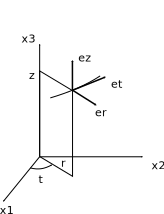
\includegraphics[height=3.5cm]{../images/T1_AnnA-0002}

\end{multicols}
\noindent Gradient et Laplacien d'une fonction scalaire:
\begin{align*}
    \grad f &= \frac{\partial f}{\partial r} \vec{e}_r + \frac{1}{r} \frac{\partial f}{\partial \theta} \vec{e}_{\theta} + \frac{\partial f}{\partial z} \vec{e}_z \\[3pt]
    \Delta f &= \frac{1}{r} \frac{\partial}{\partial r} \bigl( r \frac{\partial f}{\partial r} \bigr) + \frac{1}{r^{2}}\frac{\partial^2 f}{\partial \theta^2} + \frac{\partial^2 f}{\partial z^2}
\end{align*}
Définition des déformations:
\begin{align*}
    \varepsilon_{rr} &= \frac{\partial u_r}{\partial r} \quad \varepsilon_{\theta\theta} = \frac{1}{r} \frac{\partial u_{\theta}}{\theta} + \frac{u_r}{r} \quad \varepsilon_{zz} = \frac{\partial u_z}{\partial z} \\[3pt]
    \varepsilon_{\theta z} &= \frac{1}{2} \left\{ \frac{1}{r} \frac{\partial u_z}{\theta} + \frac{\partial u_{\theta}}{\partial z} \right\} \quad \varepsilon_{rz} = \frac{1}{2} \left\{ \frac{\partial u_r}{\partial z} + \frac{\partial u_z}{\partial r} \right\} \\[3pt]
    \varepsilon_{r\theta} &= \frac{1}{2} \left\{ \frac{\partial u_{\theta}}{\partial r} - \frac{u_{\theta}}{r} + \frac{1}{r} \frac{\partial u_r}{\partial \theta} \right\}
\end{align*}
Equations d'équilibre:
\begin{align*}
    \frac{\partial \sigma_{rr}}{\partial r} + \frac{1}{r} \frac{\partial \sigma_{r\theta}}{\partial \theta} + \frac{\partial \sigma_{rz}}{\partial z} + \frac{\sigma_{rr} - \sigma_{\theta\theta}}{r} + f_r &=0\\[3pt]
    \frac{\partial \sigma_{r\theta}}{\partial r} + \frac{1}{r} \frac{\partial \sigma_{\theta\theta}}{\partial \theta} + \frac{\partial \sigma_{\theta z}}{\partial z} + \frac{2\sigma_{r\theta}}{r} + f_{\theta} &=0\\[3pt]
    \frac{\partial \sigma_{rz}}{\partial r} + \frac{1}{r} \frac{\partial \sigma_{\theta z}}{\partial \theta} + \frac{\partial \sigma_{zz}}{\partial z} + \frac{\sigma_{rz}}{r} + f_z &=0
\end{align*}
\subsection{Coordonnées sphériques}
\begin{multicols}{2}
\noindent Repère local: $(\vec{e}_r,\vec{e}_{\theta},\vec{e}_{\phi})$
    \begin{displaymath}
        \vec{u} = 
        \begin{bmatrix}
            u_r \\
            u_{\theta} \\
            u_{\phi}
        \end{bmatrix}, \quad
        \mathbb{\sigma} = 
        \begin{bmatrix}
            \sigma_{rr} & \sigma_{r\theta} & \sigma_{r\phi} \\
            \sigma_{r\theta} & \sigma_{\theta\theta} & \sigma_{\theta\phi} \\
            \sigma_{r\phi} & \sigma_{\theta\phi} & \sigma_{\phi\phi} \\
        \end{bmatrix}
    \end{displaymath}

    \columnbreak

    \psfrag{x1}{$x_1$}
    \psfrag{x2}{$x_2$}
    \psfrag{x3}{$x_3$}
    \psfrag{er}{$\vec{e}_r$}
    \psfrag{et}{$\vec{e}_{\theta}$}
    \psfrag{ep}{$\vec{e}_{\phi}$}
    \psfrag{r}{$r$}
    \psfrag{t}{$\theta$}
    \psfrag{p}{$\phi$}
    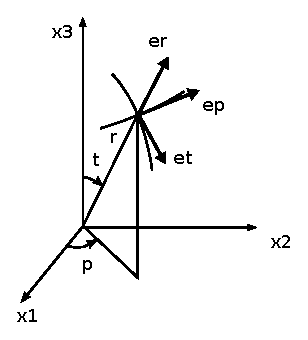
\includegraphics[height=3.5cm]{../images/T1_AnnA-0003}

\end{multicols}
\noindent Gradient et Laplacien d'une fonction scalaire:
\begin{align*}
    \grad f &= \frac{\partial f}{\partial r} \vec{e}_r + \frac{1}{r} \frac{\partial f}{\partial \theta} \vec{e}_{\theta} + \frac{1}{r\sin \theta} \frac{\partial f}{\partial \phi} \vec{e}_{\phi} \\[3pt]
    \Delta f &= \frac{1}{r^2} \frac{\partial}{\partial r} \bigl( r^2 \frac{\partial f}{\partial r} \bigr) + \frac{1}{r\sin \theta} \frac{\partial}{\partial \theta}\bigl( \frac{\sin \theta}{r} \frac{\partial f}{\partial \theta} \bigr) + \frac{1}{r\sin \theta}\frac{\partial f}{\partial \phi} \bigl( \frac{1}{r\sin \theta} \frac{\partial f}{\partial \phi} \bigr)
\end{align*}
Définition des déformations:
\begin{align*}
    \varepsilon_{rr} &= \frac{\partial u_r}{\partial r} \quad \varepsilon_{\theta\theta} = \frac{1}{r} \frac{\partial u_{\theta}}{\theta} + \frac{u_r}{r} \quad \varepsilon_{\phi\phi} = \frac{1}{r \sin \theta} \frac{\partial u_{\phi}}{\partial \phi} + \frac{u_{\theta}}{r}\cot \theta + \frac{u_r}{r} \\[3pt]
    \varepsilon_{\theta \phi} &= \frac{1}{2r} \left\{ \frac{\partial u_{\phi}}{\theta} - u_{\phi} \cot \theta \right\} + \frac{1}{2r\sin \theta} \frac{\partial u_{\theta}}{\partial \phi} \\[3pt]
    \varepsilon_{r\phi} &= \frac{1}{2} \left\{ \frac{1}{r \sin \theta} \frac{\partial u_r}{\partial \phi} + \frac{\partial u_\phi}{\partial r} - \frac{u_{\phi}}{r}\right\} \\[3pt]
    \varepsilon_{r\theta} &= \frac{1}{2} \left\{ \frac{\partial u_{\theta}}{\partial r} - \frac{u_{\theta}}{r} + \frac{1}{r} \frac{\partial u_r}{\partial \theta} \right\}
\end{align*}
Equations d'équilibre:
\begin{align*}
    \frac{\partial \sigma_{rr}}{\partial r} + \frac{1}{r} \frac{\partial \sigma_{r\theta}}{\partial \theta} + \frac{1}{r \sin \theta} \frac{\partial \sigma_{r\phi}}{\partial \phi} + \frac{2 \sigma_{rr} - \sigma_{\theta\theta} -\sigma_{\phi\phi} +\sigma_{r\theta} \cot \theta}{r} + f_r &=0\\[3pt]
    \frac{\partial \sigma_{r\theta}}{\partial r} + \frac{1}{r} \frac{\partial \sigma_{\theta\theta}}{\partial \theta} + \frac{\partial \frac{1}{r \sin \theta} \sigma_{\theta \phi}}{\partial \phi} + \frac{1}{r} \left[ \bigl( \sigma_{\theta\theta} -\sigma_{\phi\phi} \bigr)\cot\theta +3\sigma_{r\theta} \right]+ f_{\theta} &=0\\[3pt]
    \frac{\partial \sigma_{r\phi}}{\partial r} + \frac{1}{r} \frac{\partial \sigma_{\theta \phi}}{\partial \theta} + \frac{1}{r \sin \theta} \frac{\partial \sigma_{\phi\phi}}{\partial \phi} + \frac{1}{r}\bigl( 3\sigma_{r\phi} + 2 \sigma_{\theta\phi}\cot \theta \bigr) + f_\phi &=0
\end{align*}

\end{document}
